\chapter{Calorimeter Optimisation Studies}
\label{chap:detopt}

\chapterquote{The simple believes everything, but the prudent gives thought to his steps.}
{Proverbs 14:15}

%========================================================================================
%========================================================================================

\section{Calorimeter Optimisation Studies}
\label{sec:optimisationstudies}
The fundamental principle of particle flow calorimetry is to measure the energy of a particle passing through a detector in whichever sub-detector offers the best energy resolution.  For particle colliders experiments, this involves measuring the momenta of charged particles using the curvature of the track they create in the detector.  This offers extremely good energy resolution in comparison to calorimetric energy measurements and is the source of the excellent energy resolution particle flow calorimetry can produce.  As neutral particles produce no tracks, their energies must be measured using calorimetric energy deposits.  

The application of particle flow calorimetry is extremely challenging as it is possible, by using incorrect associations of charged particle tracks to calorimetric energy deposits, to both double count and omit energy measurements.  For example, if a charged particle calorimetric energy deposit is not associated to a track that energy deposit will be double counted, while if a neutral particle calorimetric energy deposit is associated to a track that energy deposit will be neglected.  Therefore, making the correct associations between charged particle tracks and calorimetric energy deposits is essential.  

These associations can only be successfully made if the calorimeters in use have fine segmentation, such as those found at the linear collider experiment, so that it becomes possible to separate the energy deposits from nearby showering particles.  Even with this segmentation making the association of charged particle tracks to the calorimetric energy deposits is highly non-trivial.  At the linear collider experiment, these associations are made using sophisticated pattern recognition algorithms, provided by PandoraPFA.  The fine segmentation of the calorimeters allows PandoraPFA to reconstruct the four-momenta of all particles passing through the detector and to use the energy measurement from the optimal sub-detector in each case. 

In this chapter optimisation of the calorimeters used at the linear collider, with focus placed on obtaining the best energy resolution for jets, is considered.  Parameters such as the number of layers, cell size and material choices for the calorimeters are considered.  

This chapter concludes with an optimisation of several global parameters for the detector such as the magnetic field strength used for the detector and the inner radius of the ECal.  These parameters are not calorimeter specific, but affect the jet energy resolution obtained from particle flow. 

%========================================================================================
%========================================================================================

\section{Jet Energy Resolution}
\label{sec:optstudiesmetric}
As many physics processes of interest at the linear collider involve multi-jet final states, good jet energy resolution is a crucial a aspect of detector performance.  As shown in chapter PHYSICS ANALYSIS, parameters derived from the energy measurements of jets, such as invariant mass, are extremely useful for identification of physics channels of interest as well as determining the sensitivity of the linear collider experiments to areas of new physics.  Therefore, the primary metric used in this study is the jet energy resolution.

Jet energy resolution in particular can benefit from the application of particle flow calorimetry as $\approx 70 \%$ of the energy of jets are carried in the from of charged particles.  As particle flow aims to measure the energy of charged particles using the tracker, it has the potential to offers extremely large benefits when measuring jet energies in comparison to the traditional calorimetric approach.  

%========================================================================================

\subsection{Jet Energy Resolution Metrics}
\begin{figure}
\centering
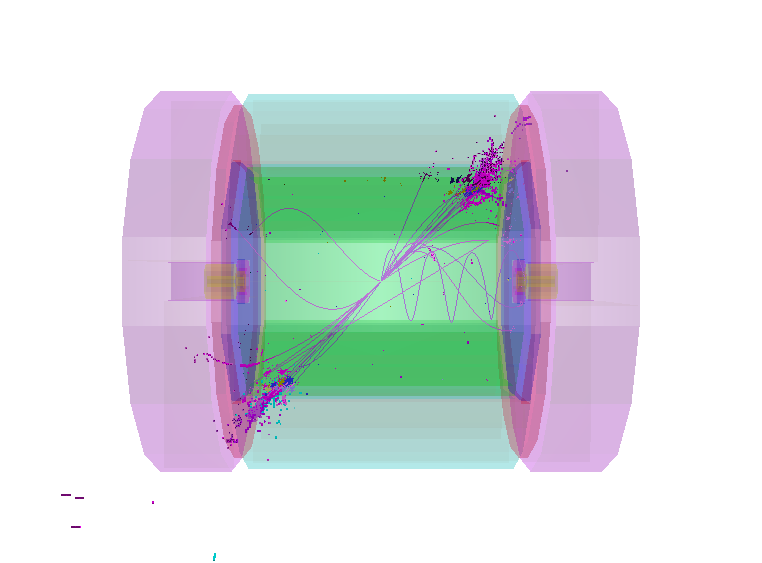
\includegraphics[width=0.5\textwidth]{OptimisationStudies/Plots/MethodDescription/500GeVEvent.png}
\caption[500 GeV di-jet Z$\rightarrow$uds event display for nominal ILD detector.]{500 GeV di-jet Z$\rightarrow$uds event display for nominal ILD detector.}
\label{fig:500GeVzudsevtdisplay}
\end{figure} 

The primary metric used to optimise detector performance is the jet energy resolution.  This was found through the simulation of off-shell mass Z boson events decaying to light quarks (u, d, s).  In these events the Z boson is produced at rest, which means the typical decays form two mono-energetic jets that are produced back to back as shown in figure \ref{fig:500GeVzudsevtdisplay}.  Only events where $|\text{cos}(\theta)| < 0.7$, where $\theta$ is the polar angle of the quarks from the Z decay, are used in the metric calculation to ensure little energy is lost down the beam axis.  Using these events the jet energy resolution is calculated as follows: 

\begin{equation} 
\frac{\text{RMS}_{90}(E_{i})}{\text{Mean}_{90}(E_{i})} = \frac{\text{RMS}_{90}(E_{jj})}{\text{Mean}_{90}(E_{jj})} \times \sqrt{2} \text{,}
\end{equation}

\begin{flushleft}
where $\text{RMS}_{90}(E_{jj})$ and $\text{Mean}_{90}(E_{jj})$ are the root mean squared (RMS) and the mean of the reconstructed energy distribution calculated within the range of with the smallest RMS containing at least 90\% of the data.
respectively.
\end{flushleft}

\begin{figure}
\centering
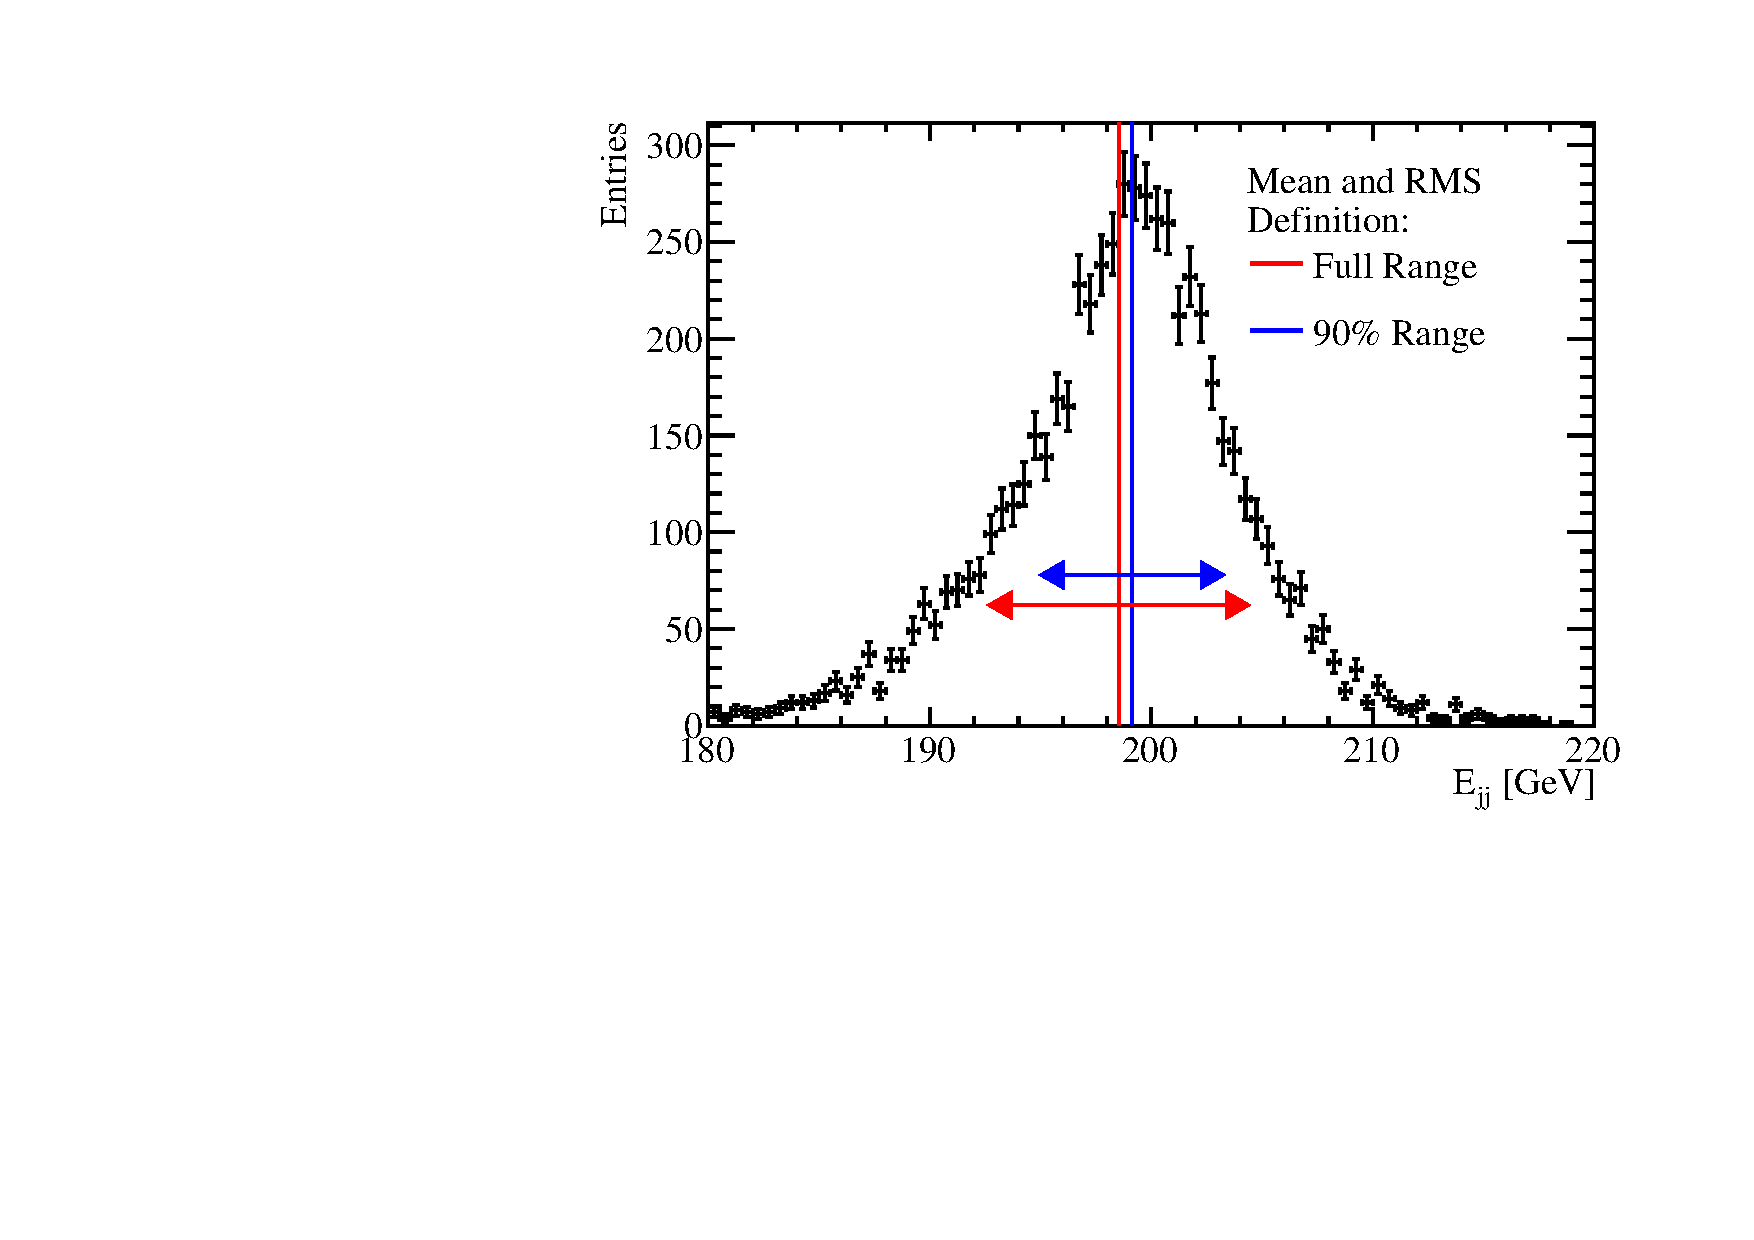
\includegraphics[width=0.5\textwidth]{OptimisationStudies/Plots/MethodDescription/RMS90Plot.pdf}
\caption[Definition of jet energy resolution.   Reconstructed jet energy for 200 GeV di-jet Z$\rightarrow$uds events for nominal ILD detector.]{Definition of jet energy resolution.   Reconstructed jet energy for 200 GeV di-jet Z$\rightarrow$uds events for nominal ILD detector.}
\label{fig:rms90defintion}
\end{figure} 

This definition is used to remove the effect of outliers in the distribution \cite{arXiv:0907.3577}.  Although the correct combination of charged particle tracks and calorimetric energy measurements would give a Gaussian reconstructed jet energy distribution, the effect of confusion on certain events will distort this distribution and broaden the tails significantly.  If the full range were to be used in the jet energy resolution calculation, the effect of these tails is overinflated.  If the distribution of reconstructed jet energies is truncated to the narrowest range of the data containing at least $90\%$ of the data, the effect of these tails can be negated.  This removes events where confusion is dominant, which makes the jet energy resolution metric far more robust and representative of the bulk of the data.  

An example of the application of this metric can be found in figure \ref{fig:rms90defintion}.  The RMS calculated using the full range 5.8 GeV, while the RMS using the reduced range is 4.1 GeV.  This corresponds to a reduction in the jet energy resolution from $4.1\%$ to $2.9\%$, which clearly shows an overemphasis of the tails of the distribution if the full range is used in the calculation.

In the subsequent analysis a range of di-jet energies were considered ranging from the Z mass, 91 GeV, to the nominal running energy of the ILC, 500 GeV.  Each event sample contained 10,000 events generated spatially isotropically so that, given the polar angle cut, approximately 7,000 events contribute to the jet energy resolution metric. 

%========================================================================================

\subsection{Jet Energy Resolution Decompositions}
The pattern recognition performed for the linear collider experiments is full described in section PANDORA SECTION, however, it is possible to gain further insight into the detector performance by cheating various parts of the pattern recognition using the MC information.  Pattern recognition confusion manifests itself on energy measurements in two ways:

\begin{itemize}
\item If part of the calorimetric energy deposit from a charged particle is not associated to the track that energy deposit is double counted.
\item If part of the calorimetric energy deposit from a neutral particle is incorrectly associated to a track, the energy deposit is not accounted for.
\end{itemize}

\begin{flushleft}
Both of these sources of confusion lead to inaccurate measurements of the jet energy and thus degrade the resolution.  Cheating the pattern recognition, therefore, removes the effects of confusion and improves the detector performance.  
\end{flushleft}

The intrinsic energy resolution contribution to the jet energy resolution was determined by fully cheating the pattern recognition; in this case all confusion is negated.  The total confusion is defined as the quadrature difference between the jet energy resolution using the standard reconstruction and this fully cheated reconstruction.  Furthermore, it is possible to cheat the pattern recognition associated with individual types of particles.  This is particularly useful for studies related to the ECal as, by cheating the photon pattern recognition, it is possible to isolate the confusion associated with photons.  The photon confusion is defined as the quadrature difference between the jet energy resolution using the standard reconstruction and the reconstruction where photons pattern recognition is cheated.    

%========================================================================================

\subsection{Single Particle Energy Resolution}
Several physics studies rely on the identification of single particles, such as $\gamma$ in anomalous triple gauge coupling studies CITE, and as such the energy resolution of individual particles is presented alongside the jet energy resolution metric.  As only uncharged particle energies are measured in the calorimeters in the particle flow paradigm, the single particle energy resolution is shown using $\gamma$s and for $K^{0}_{L}$s.  $\gamma$s are particularly relevant for several physics studies and, as they are largely contained within the ECal, they provide insight into detector changes related purely to the ECal.  This makes $\gamma$s a natural choice of particle to consider for this study.  $K^{0}_{L}$s were used as, analogously to $\gamma$s and the ECal, their energies are primarily measured using the HCal.  Although in general neutral hadron energy resolutions are less crucial to physics studies, the energy resolution is still a crucial contribution to the jet energy resolution, which should not be overlooked.  For these single particle samples the energy resolution is defined using a Gaussian fit to the reconstructed energy distributions.  The fit was applied to the narrowest region of the reconstructed PFO energy distribution that contained at least 75\% of the data.  This increases the likelihood that the fit converges and ensures a better parameterisation of the bulk of the data set.  The resolution is defined as the standard deviation divided by the mean of that reconstructed Gaussian.  A total of 10,000 events are used to calculate the energy resolution at each fixed energy point.  A cut of $|\text{cos}(\theta)| < 0.7$ is applied to ensure events avoid the Barrel/EndCap overlap region.  Examples of the single particle energy distributions for 100 GeV $\gamma$s and 50 GeV $K^{0}_{L}$s alongside the Gaussian fit used to determine their energy resolution are shown in figure \ref{fig:singleparticleenergyhists}.  The errors quoted on single particle energy resolutions are determined by propagating the errors reported from the Gaussian fit into the resolution calculation.  

\begin{figure}
\centering
\subfloat[50 GeV $K^{0}_{L}$.]{\label{fig:kaonsingleparticleenergyhist}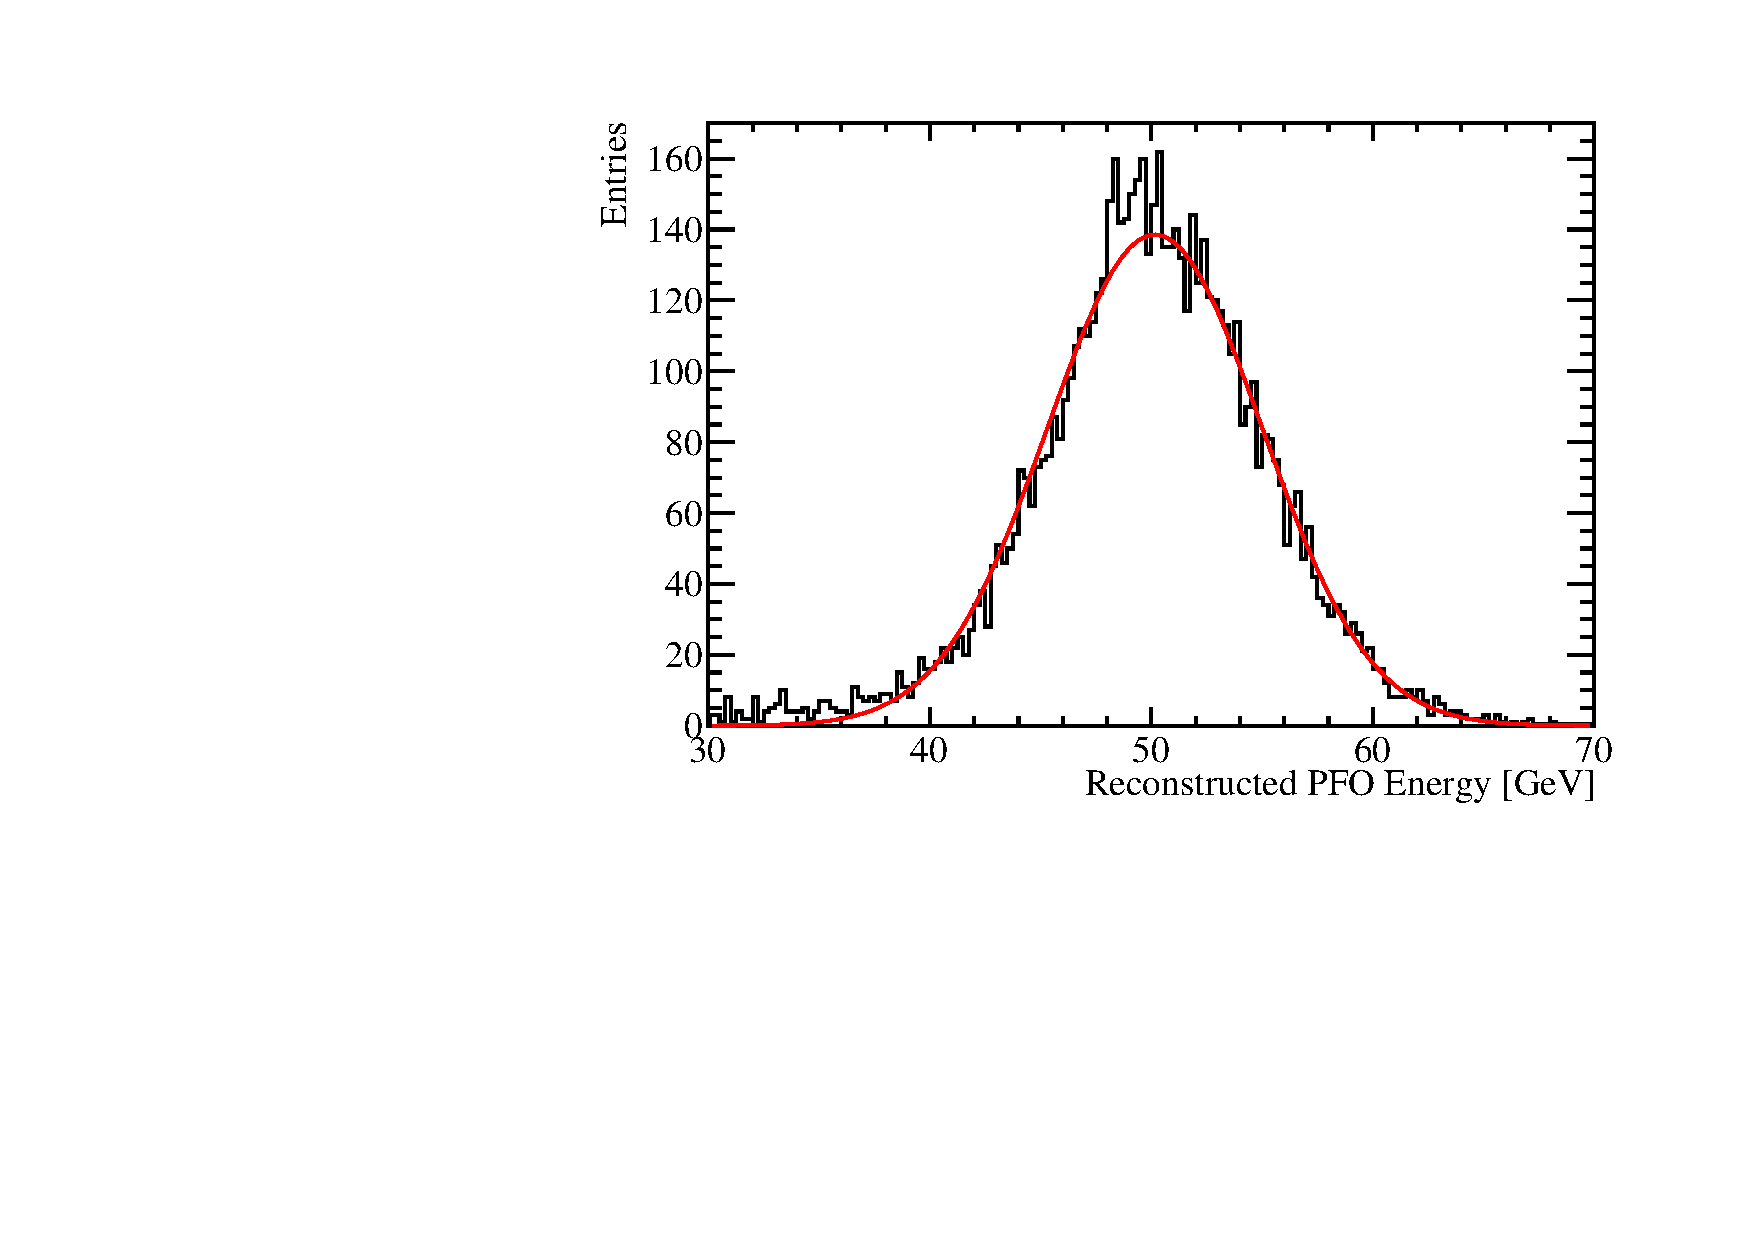
\includegraphics[width=0.5\textwidth]{OptimisationStudies/Plots/EnergyResolution/EKaon0L_50GeV.pdf}}
\subfloat[100 GeV $\gamma$.]{\label{fig:photonsingleparticleenergyhist}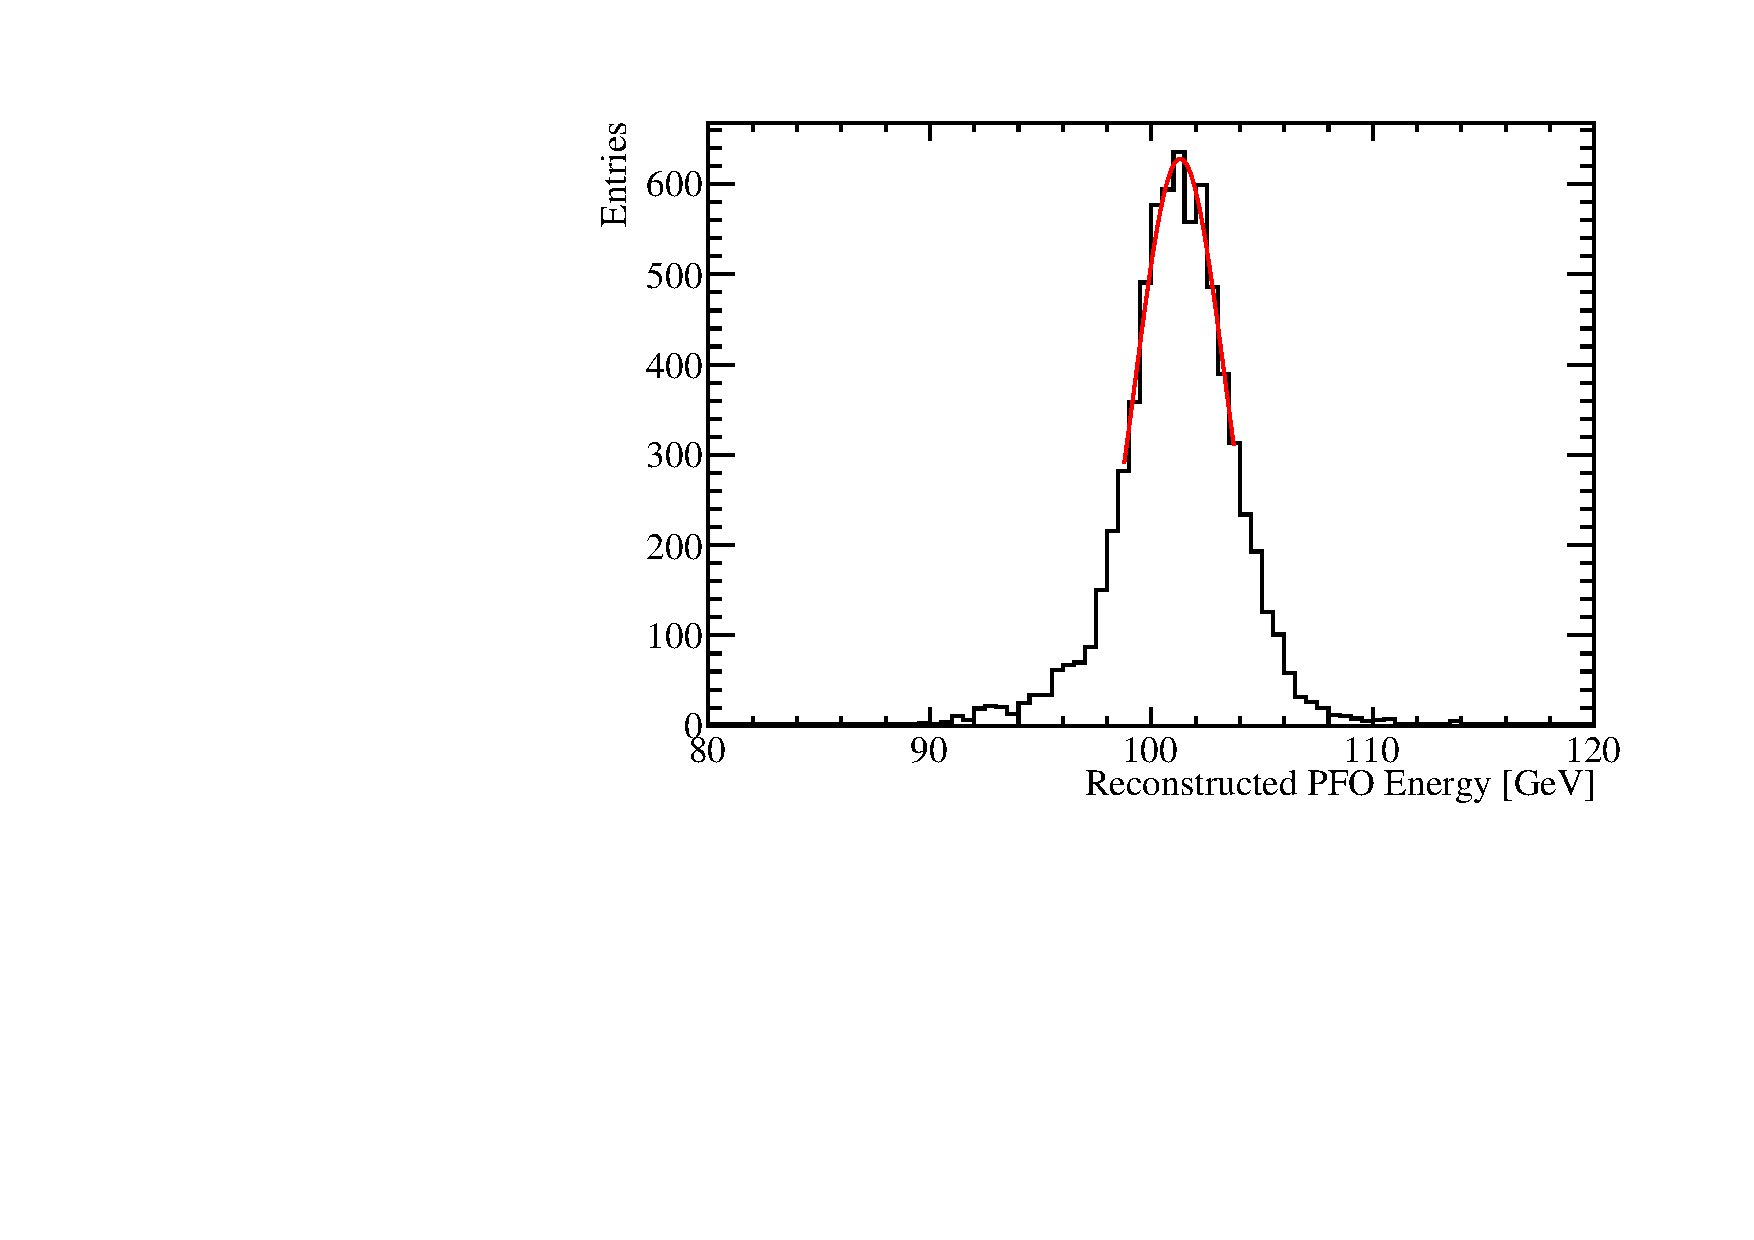
\includegraphics[width=0.5\textwidth]{OptimisationStudies/Plots/EnergyResolution/EPhoton_100GeV.pdf}}
\caption[The reconstructed energy distribution for \protect\subref{fig:kaonsingleparticleenergyhist} 50 GeV $K^{0}_{L}$ and \protect\subref{fig:photonsingleparticleenergyhist} 100 GeV $\gamma$ events.  The red line shows a Gaussian fit used to parameterise the detector performance.  The fit was applied to the truncated range of the reconstructed PFO energy distribution containing at least 75\% of the data with the narrowest RMS.  The nominal ILD model was used in this simulation.]{The reconstructed energy distribution for \protect\subref{fig:kaonsingleparticleenergyhist} 50 GeV $K^{0}_{L}$ and \protect\subref{fig:photonsingleparticleenergyhist} 100 GeV $\gamma$ events.  The red line shows a Gaussian fit used to parameterise the detector performance.  The fit was applied to the truncated range of the reconstructed PFO energy distribution containing at least 75\% of the data with the narrowest RMS.  The nominal ILD model was used in this simulation.}
\label{fig:singleparticleenergyhists}
\end{figure}

%========================================================================================
%========================================================================================

\section{Nominal Detector Performance}
Before addressing the optimisation of the detectors for use at a future linear collider is it necessary to properly quantify the behaviour of the nominal detector model that is used in the simulations.  For these studies the nominal ILD model is used.  

The calorimeters at a linear collider are sampling calorimeters, therefore, the reconstructed energy distributions for neutral particles whose energies are measured in the calorimeters will be Gaussian.  This is expected due as the active material for each calorimeter cell essentially counts the number of charged particle tracks passing through it, or possible the number of photons for scintillator options.  The working hypothesis for estimating the energy deposited in a sampling calorimeter is that the energy of a showering particle is proportional to the number of charged particle tracks, or photons for scintillator detector options, it produces.  Having counted the number of tracks in the active region of the calorimeter cell it is possible to estimate the energy deposited in the whole calorimeter cell in the digitisation process, further details on this can be found in chapter CALIBRATION CHAPTER.  Finally, the energy of the entire particle shower is estimated by grouping the calorimeter cells and summing their energy.  Each calorimeter cell energy is an independently random measurements and, by the central limit theorem CITE, the sum of a large number of independently random measurements has a Gaussian distribution.  It follows that the variance of the shower energy distribution is given by the sum of the variances for each of the calorimeter cell energy distributions.  

As each calorimeter hit involves counting a number of objects, charged particle tracks or photons, the statistics governing the distribution of the individual cell energies are Poisson statistics.  For a given particle shower, if the mean of a cell energy is given by $\lambda = N$ where $N$ is the mean number of objects that are expected, the standard deviation of that distribution is $\sigma = \sqrt{\lambda} = \sqrt{N}$ and the energy resolution $\frac{\sigma}{\lambda} = \frac{1}{\sqrt{N}}$.  As the total shower energy, $E_{Reco}$, is proportional to $N_{Reco}$, the total number of tracks recorded in the calorimeter, the energy resolution for an ideal calorimeter is proportional to $\frac{1}{\sqrt{N_{Reco}}} = \frac{1}{\sqrt{E_{Reco}}}$.  This gives the form of the energy resolution as a function of energy for an ideal calorimeter as $\frac{\sigma_{Reco}}{E_{Reco}} = \frac{a}{\sqrt{E_{Reco}}}$.  In reality, it is typical to express the energy resolution of a calorimeter in the following form

\begin{equation} 
\frac{\sigma_{Reco}}{E_{Reco}} = \frac{a}{\sqrt{E_{Reco}}} \oplus b \oplus \frac{c}{E_{Reco}}\text{,}
\end{equation}

\begin{flushleft}
where the $b$ term is a constant term that accounts for a variety of effects such as CHECK and the $c$ term accounts for electrical noise.
\end{flushleft}

Prototypes of the various ILD calorimeter options have been constructed and validated using test beam.  The energy resolution measured using the test beam was parameterised as $\frac{16.6}{\sqrt{E_{Reco}}} \oplus 1.1 \%$ for the silicon ECal and $\frac{12.9}{\sqrt{E_{Reco}}} \oplus 1.2 \%$ for the scintillator ECal \cite{Behnke:2013lya}.  The electrical noise was deemed sufficiently small that the $c$ term in the parameterisation could be neglected in both cases.  These results were determined using an $\text{e}^{-}$ test beam with energies ranging up to $\approx 40$ GeV.  This parametrisation is compared to the results found using the full ILD detector simulation in figures \ref{fig:ecalsinominalres} and \ref{fig:ecalscnominalres} for the silicon and scintillator ECal options respectively.  The parameterisation of the energy resolution for the silicon ECal option is almost identical to the energy resolution results when using the full ILD simulation.  However, for the scintillator ECal option the parameterisation is significantly better than that observed in the full simulation.  This difference is most likely due to an imperfect implementation of the scintillator ECal within the full detector simulation.  Even with this difference, the $\gamma$ energy resolutions measured using the full ILD simulation when using the silicon and scintillator ECal options are similar.  At very high energies, $\approx 500$ GeV, the ECal is no longer sufficient to fully contain the $\gamma$s and so leakage into the HCal leads to a minor degradation the energy resolution for the full simulation.  This accounts for the deviation in the energy resolution between the full ILD simulation and the test beam parameterisation for the silicon ECal option.   

Similarly, the energy resolution using test beam was parameterised as $\frac{57.6}{\sqrt{E_{Reco}}} \oplus 1.6 \%$ for the nominal ILD HCal \cite{Adloff:2012gv}.  A comparison between this test beam parameterisation and the full ILD simulation, using the silicon ECal option, is shown in figure \ref{fig:hcalnominalres}.  The test beam used for this parameterisation used $\pi^{\pm}$s with energies ranging from 10 to 80 GeV.  In the determination of the test beam parameterisation, only showers starting in the HCal were considered whereas all showers were considered in the full ILD simulation.  Negating showers starting in the ECal removes the effect of errors associated with the calibration of ECal for hadronic energy measurements and leads to a better energy resolution for the $K^{0}_{L}$.  The deviation between the test beam parameterisation and the full simulation grows at high $K^{0}_{L}$ energies due to the treatment of energy deposits leaking out of the back of the HCal.  A tail catcher was used in the test beam analysis that had a similar structure to the HCal, but with a much wider average absorber thickness.  Energy deposits in this tail catcher were calibrated in a similar fashion to the HCal giving a very good energy resolution for these energy deposits.  In the full ILD simulation a muon chamber acts as the tail catcher, however, the calibration applied to energy deposits here is far less advanced than that applied to the test beam data meaning the energy resolution for these hits will be worse.  Furthermore, energy deposits in the uninstrumented solenoid region of the full ILD simulation are not accounted for.  These lost energy deposits and simplistic calibration are the main causes of the deviation of the test beam parameterisation and the full simulation energy resolution for high energy $K^{0}_{L}$s.   

Combining these results together it is possible to demonstrate the effectiveness of particle flow calorimetry on the jet energy resolutions.  After the decay of short lived particles approximately 60\% of the energy of a jet is carried in the form of charged particles, 30\% in the form of $\gamma$s and 10\% in the form of neutral hadrons.  A negligible amount of energy is also carried in the form of invisible energy i.e. neutrinos.  In the traditional calorimetric approach the $\gamma$s are measured largely within the ECal, with an energy resolution of $\approx 0.15 \times \sqrt{E_{\gamma}}$, and the remaining particles are measured in the HCal, with an energy resolution of $\approx 0.55 \times \sqrt{E_{h}}$.  Note here that these are the raw, not fractional energy resolutions.  Therefore, the contributions to the fractional jet energy resolution are $\frac{0.08}{\sqrt{E_{j}}}$ from $\gamma$s and $\frac{0.46}{\sqrt{E_{j}}}$ from other particles where $E_{j}$ is the jet energy.  These add in quadrature to give a total jet energy resolution of $\frac{0.47}{\sqrt{E_{j}}}$.  In the particle flow paradigm the energy of charged particles is measured in the tracker, which has such a good energy resolution than the contribution to the jet energy resolution is negligible.  This means the contributions to the jet energy resolutions only come from $\gamma$s, $\frac{0.08}{\sqrt{E_{j}}}$, and from neutral hadrons, $\frac{0.17}{\sqrt{E_{j}}}$.  When added in quadrature they give a total jet energy resolution of $\frac{0.19}{\sqrt{E_{j}}}$, which is significantly better than when using the traditional calorimetric approach.  It must be emphasised that this is an upper limit on the performance as the effect of confusion will degrade the jet energy resolution.  However, by applying sophisticated pattern recognition algorithms this confusion can be minimised and exceptional performance achieved. 

The jet energy resolutions as a function of jet energy using the full ILD simulation are shown in figure \ref{fig:jernominalres}.  Alongside this the intrinsic energy resolution and confusion contributions to the jet energy resolution are also presented.  For low jet energies the jet energy resolution is dominated by the intrinsic energy resolution of the detector.  This indicates that the charged particle track to calorimeter hit cluster associations being made are largely correct and that the resolution is being driven by the energy resolution of the calorimeters.  For high jet energies the event topology is more dense and mote error are present in the track cluster associations being made.  Even at these large energies, the intrinsic energy resolution of the detector, which goes as $~\frac{1}{\sqrt{E_{j}}}$, has reduced so much that the performance at high energies is better than that observed for the low energies.  When the performance is put into context, these jet energy resolutions are sufficiently low, $\frac{\sigma_{E}}{E} \lesssim 3.8\%$ \cite{Behnke:2013lya, arXiv:0907.3577, Linssen:2012hp}, that it is possible to separate hadronic W and Z decays, which is one of the key requirements for the future linear collider.    

\begin{figure}
\centering
\subfloat[]{\label{fig:ecalsinominalres}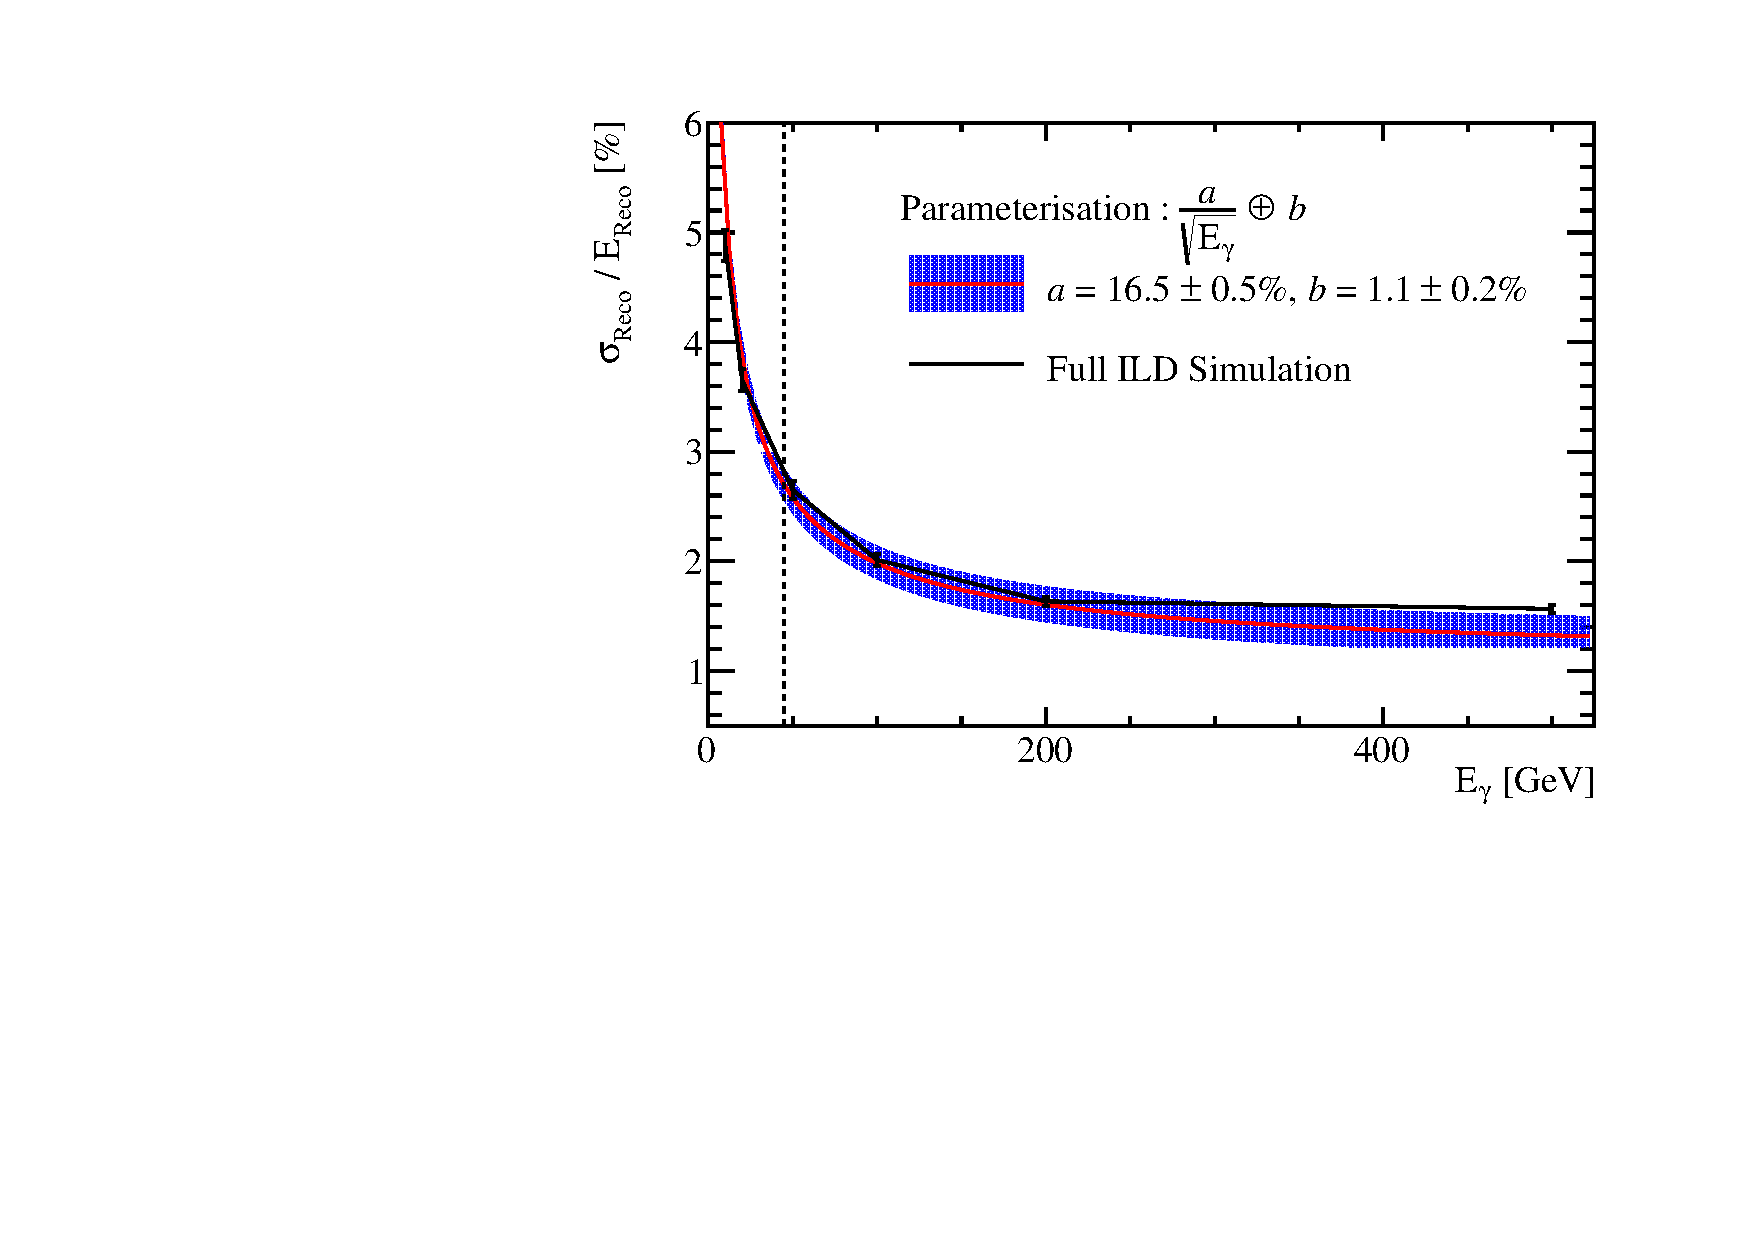
\includegraphics[width=0.5\textwidth]{OptimisationStudies/Plots/EnergyResolution/ER_vs_EGamma_SiECal.pdf}}
\subfloat[]{\label{fig:ecalscnominalres}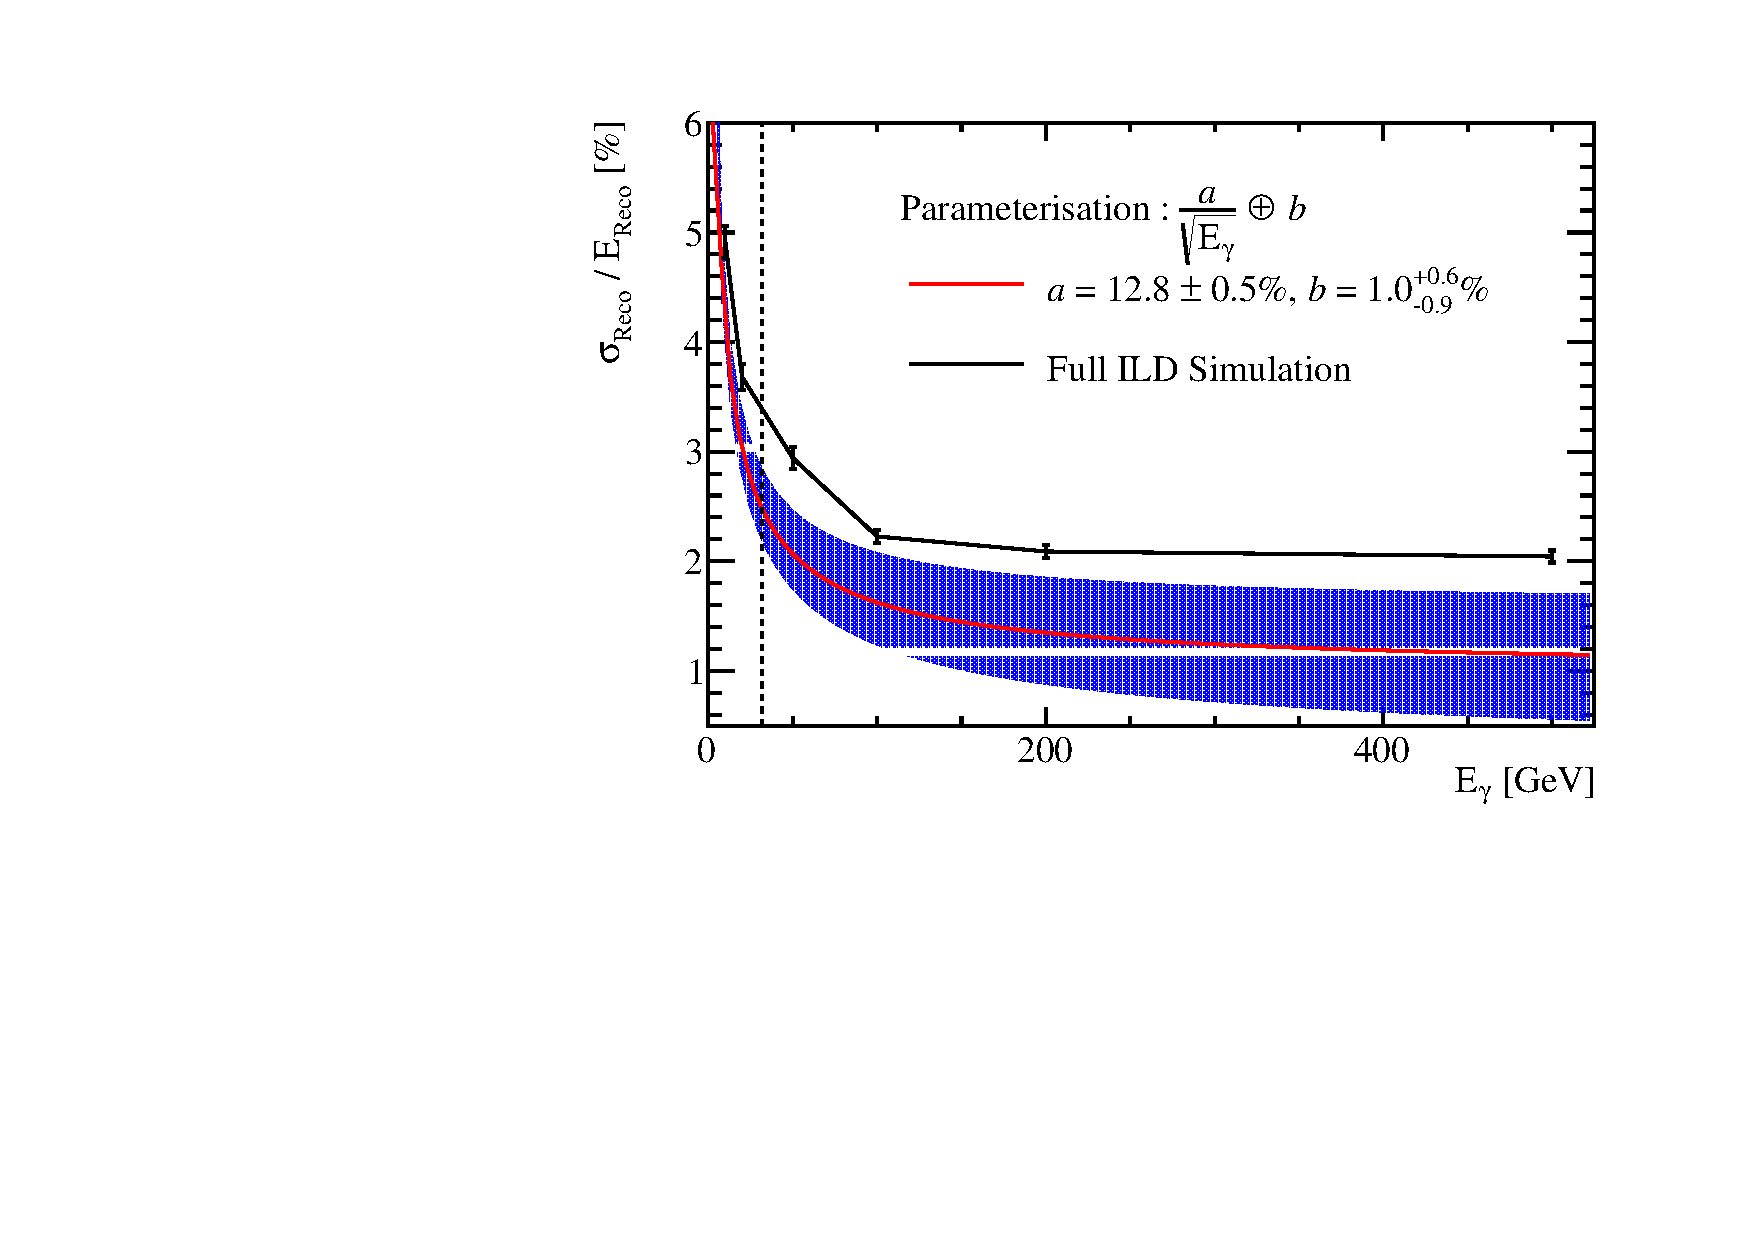
\includegraphics[width=0.5\textwidth]{OptimisationStudies/Plots/EnergyResolution/ER_vs_EGamma_ScECal.pdf}}\\
\subfloat[]{\label{fig:hcalnominalres}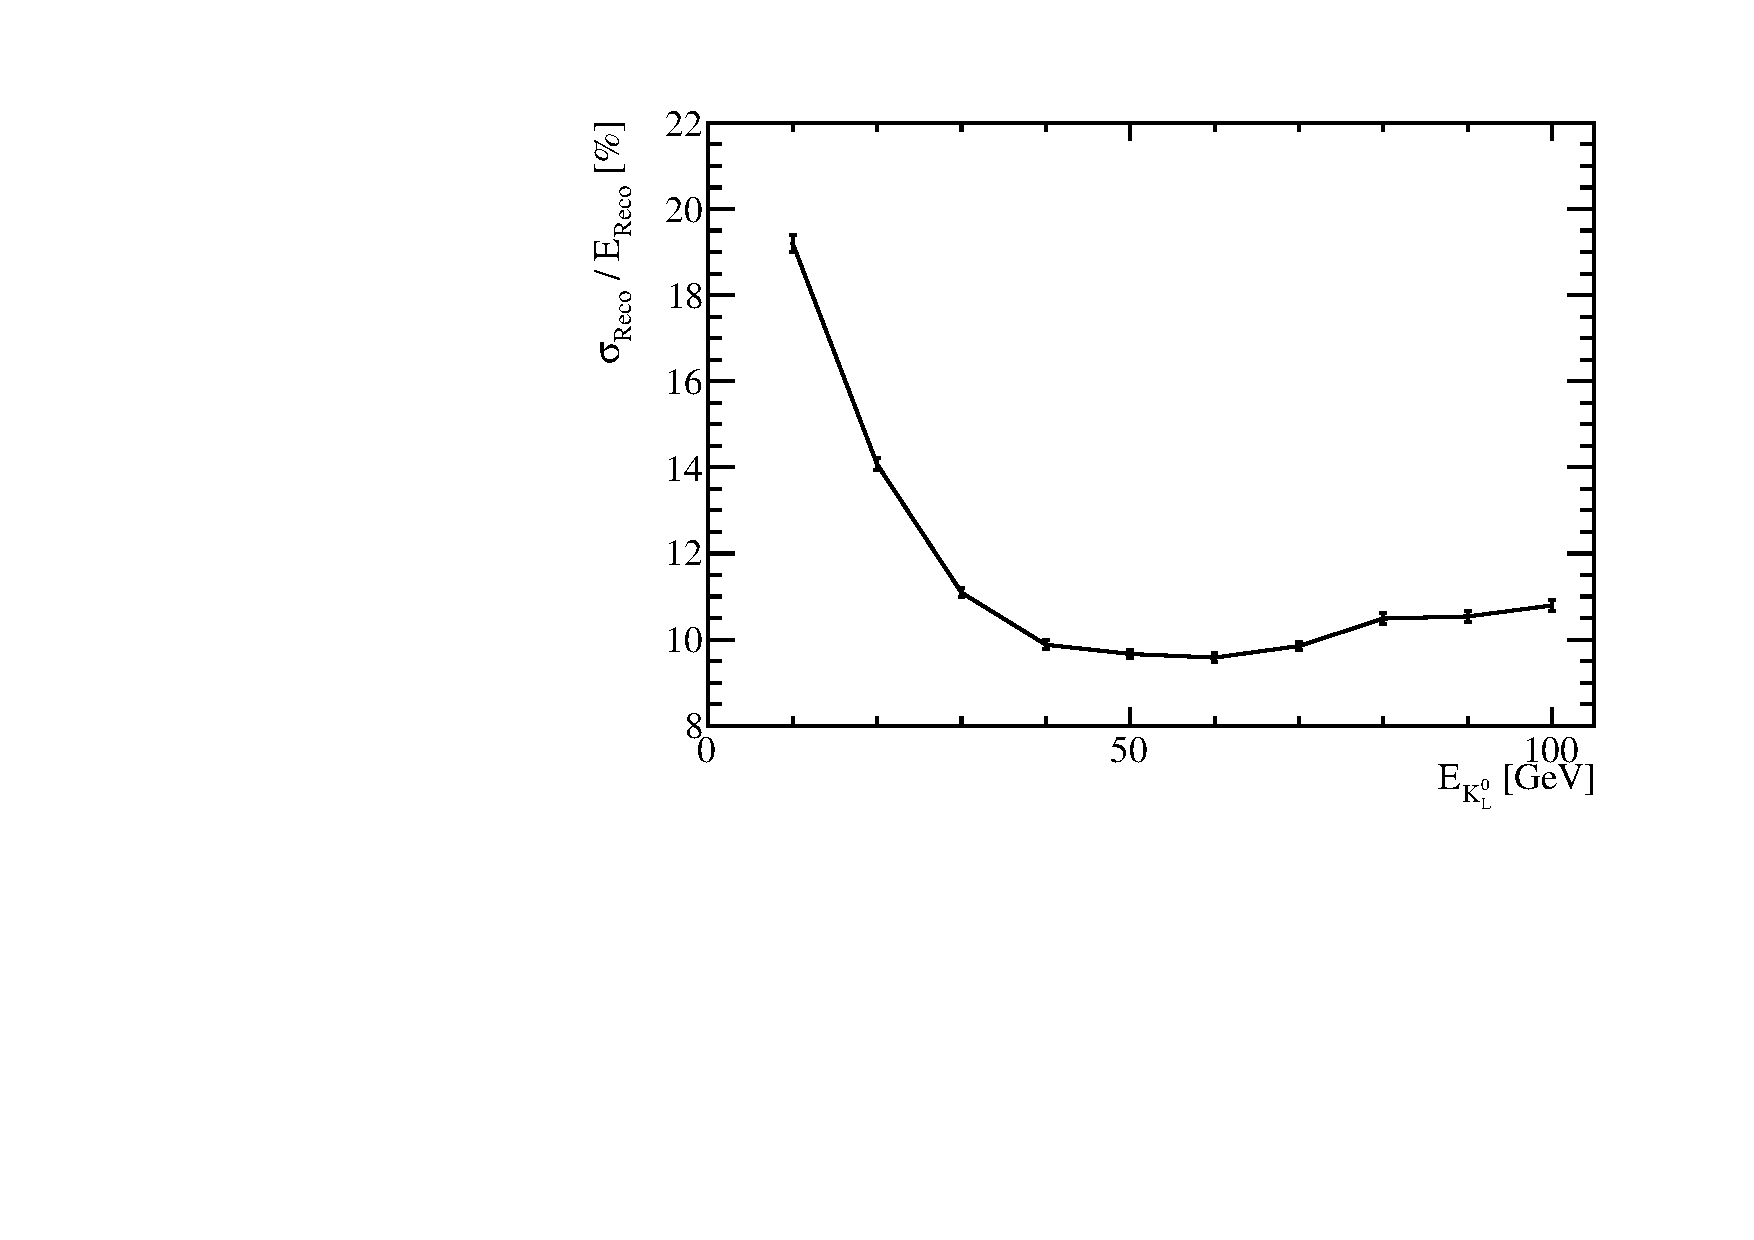
\includegraphics[width=0.5\textwidth]{OptimisationStudies/Plots/EnergyResolution/ER_vs_EKaon0L_SiECal.pdf}}
\subfloat[]{\label{fig:jernominalres}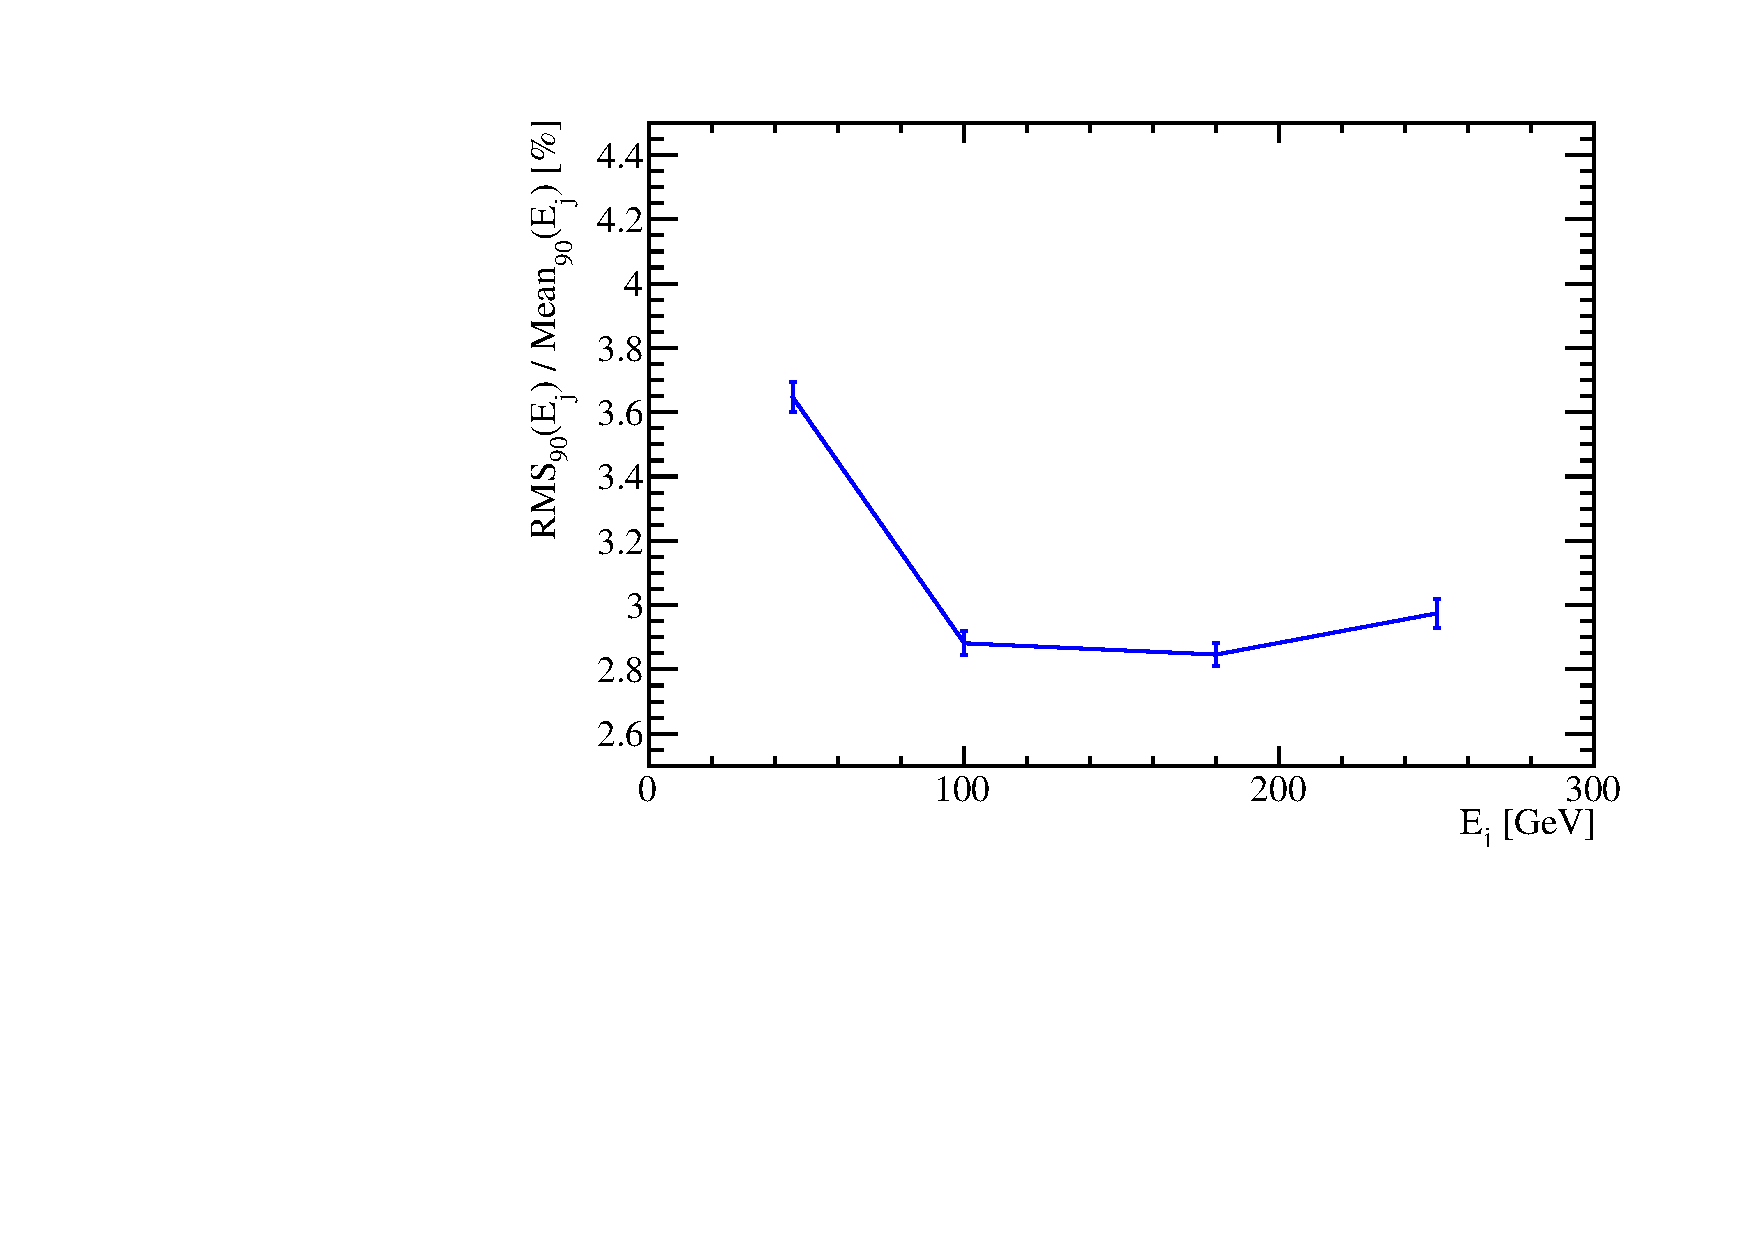
\includegraphics[width=0.5\textwidth]{OptimisationStudies/Plots/JetEnergyResolutions/JER_vs_JetEnergy_NominalDetectorPerformance.pdf}}
\caption[\protect\subref{fig:ecalsinominalres} The energy resolution as a function of $\gamma$ energy using the nominal ILD model for the silicon ECal option.  \protect\subref{fig:ecalscnominalres} The energy resolution as a function of $\gamma$ energy using the nominal ILD model for the scintillator ECal option.  \protect\subref{fig:hcalnominalres} The energy resolution as a function of $K^{0}_{L}$ energy using the nominal ILD model with the silicon ECal option.  \protect\subref{fig:jernominalres} The jet energy resolution ($\text{RMS}_{90}$) as a function of jet energy using the nominal ILD model with the silicon ECal option.  The intrinsic energy resolution and confusion contributions these the jet energy resolutions are also presented.  The black dotted line on the single particle energy resolutions shows the highest energy particles used in the test beam measurements.]{\protect\subref{fig:ecalsinominalres} The energy resolution as a function of $\gamma$ energy using the nominal ILD model for the silicon ECal option.  \protect\subref{fig:ecalscnominalres} The energy resolution as a function of $\gamma$ energy using the nominal ILD model for the scintillator ECal option.  \protect\subref{fig:hcalnominalres} The energy resolution as a function of $K^{0}_{L}$ energy using the nominal ILD model with the silicon ECal option.  \protect\subref{fig:jernominalres} The jet energy resolution ($\text{RMS}_{90}$) as a function of jet energy using the nominal ILD model with the silicon ECal option.  The intrinsic energy resolution and confusion contributions these the jet energy resolutions are also presented.  The black dotted line on the single particle energy resolutions shows the highest energy particles used in the test beam measurements.}
\label{fig:nominalres}
\end{figure}

%========================================================================================
%========================================================================================

\section{Electromagnetic Calorimeter Optimisation}
\label{sec:ecal}
The ECal primarily measures the energy deposits of electromagnetic showers.  The ECal in the nominal ILD detector model, summarised in table \ref{table:defaultildecal}, is a silicon-tungsten sampling calorimeter.  It contains 24 radiation lengths ($\text{X}_{0}$), which is sufficient to contain all but the highest energy electromagnetic showers, and has 29 readout layers.  The absorber thickness of the last nine layers is twice that of the first 20 layers to reduces the number of readout channels and cost of the overall calorimeter while retaining a high sampling rate.  This high sampling rate is crucial for the pattern recognition aspect of particle flow calorimetry, especially in the region where particle showers start developing, as shown in section \ref{sec:ecalcells}.  

\begin{table}[h!]
\centering
\begin{tabular}{ l l}
\hline
Parameter & Default Value \\
\hline
Cell Size & $5 \times 5 \text{mm}^{2}$ square cells \\
Number of Layers & 29 readout layers \\
Active Material Choice & Silicon or Scintillator  \\
Active Material Thickness & 0.5 mm (Silicon) or 2 mm (Scintillator)  \\
Absorber Material Choice & Tungsten \\
Absorber Material Thickness & 20 layers of 2.1 mm followed by 9 layers of 4.2 mm \\
\hline
\end{tabular}
\caption[The configuration of the ECal in the nominal ILD detector model.  The parameters are given for the nominal silicon model as well as the alternative scintillator option.]{The configuration of the ECal in the nominal ILD detector model.  The parameters are given for the nominal silicon model as well as the alternative scintillator option.}
\label{table:defaultildecal}
\end{table}

The calorimeter performance was simulated for a number of detector models where the following detector parameters were varied:
\begin{itemize}
\item Cell size.  This is a vital aspect of the detector in the particle flow paradigm as smaller cell sizes give greater potential for being able to separate energy deposits from charged and neutral particles.  This should have little to no effect on the intrinsic energy resolution of the detector.  
\item Number of layers or sampling frequency.  In this study the layer thicknesses are varied to keep the total number of radiation lengths within the detector constant.  By increasing the number of layers in the calorimeter a particle shower is sampled more thoroughly leading to a reduction in the stochastic contribution to the energy resolution.  Therefore, the number of layers will governs the intrinsic energy resolution of the calorimeter.
\item Active material choice, with the option of either silicon or scintillator as the active medium.  As well as providing different intrinsic energy resolutions the readout mechanics of these two options are significantly different.  There is no clear prior knowledge as to which should provide better performance. 
\end{itemize}

%========================================================================================

\subsection{ECal Cell Size}
\label{sec:ecalcells}
A number of different detector models were considered where the cell size in the ECal was varied about the nominal value of $5 \times 5 \text{mm}^{2}$ square cells.  The granularities considered were $3 \times 3 \text{mm}^{2}$, $5 \times 5 \text{mm}^{2}$, $7 \times 7 \text{mm}^{2}$, $10 \times 10 \text{mm}^{2}$, $15 \times 15 \text{mm}^{2}$ and $20 \times 20 \text{mm}^{2}$ square cells for both the silicon and scintillator active material options.  

% SP
\begin{figure}
\centering
\subfloat[]{\label{fig:ecalsicellsize100gamma}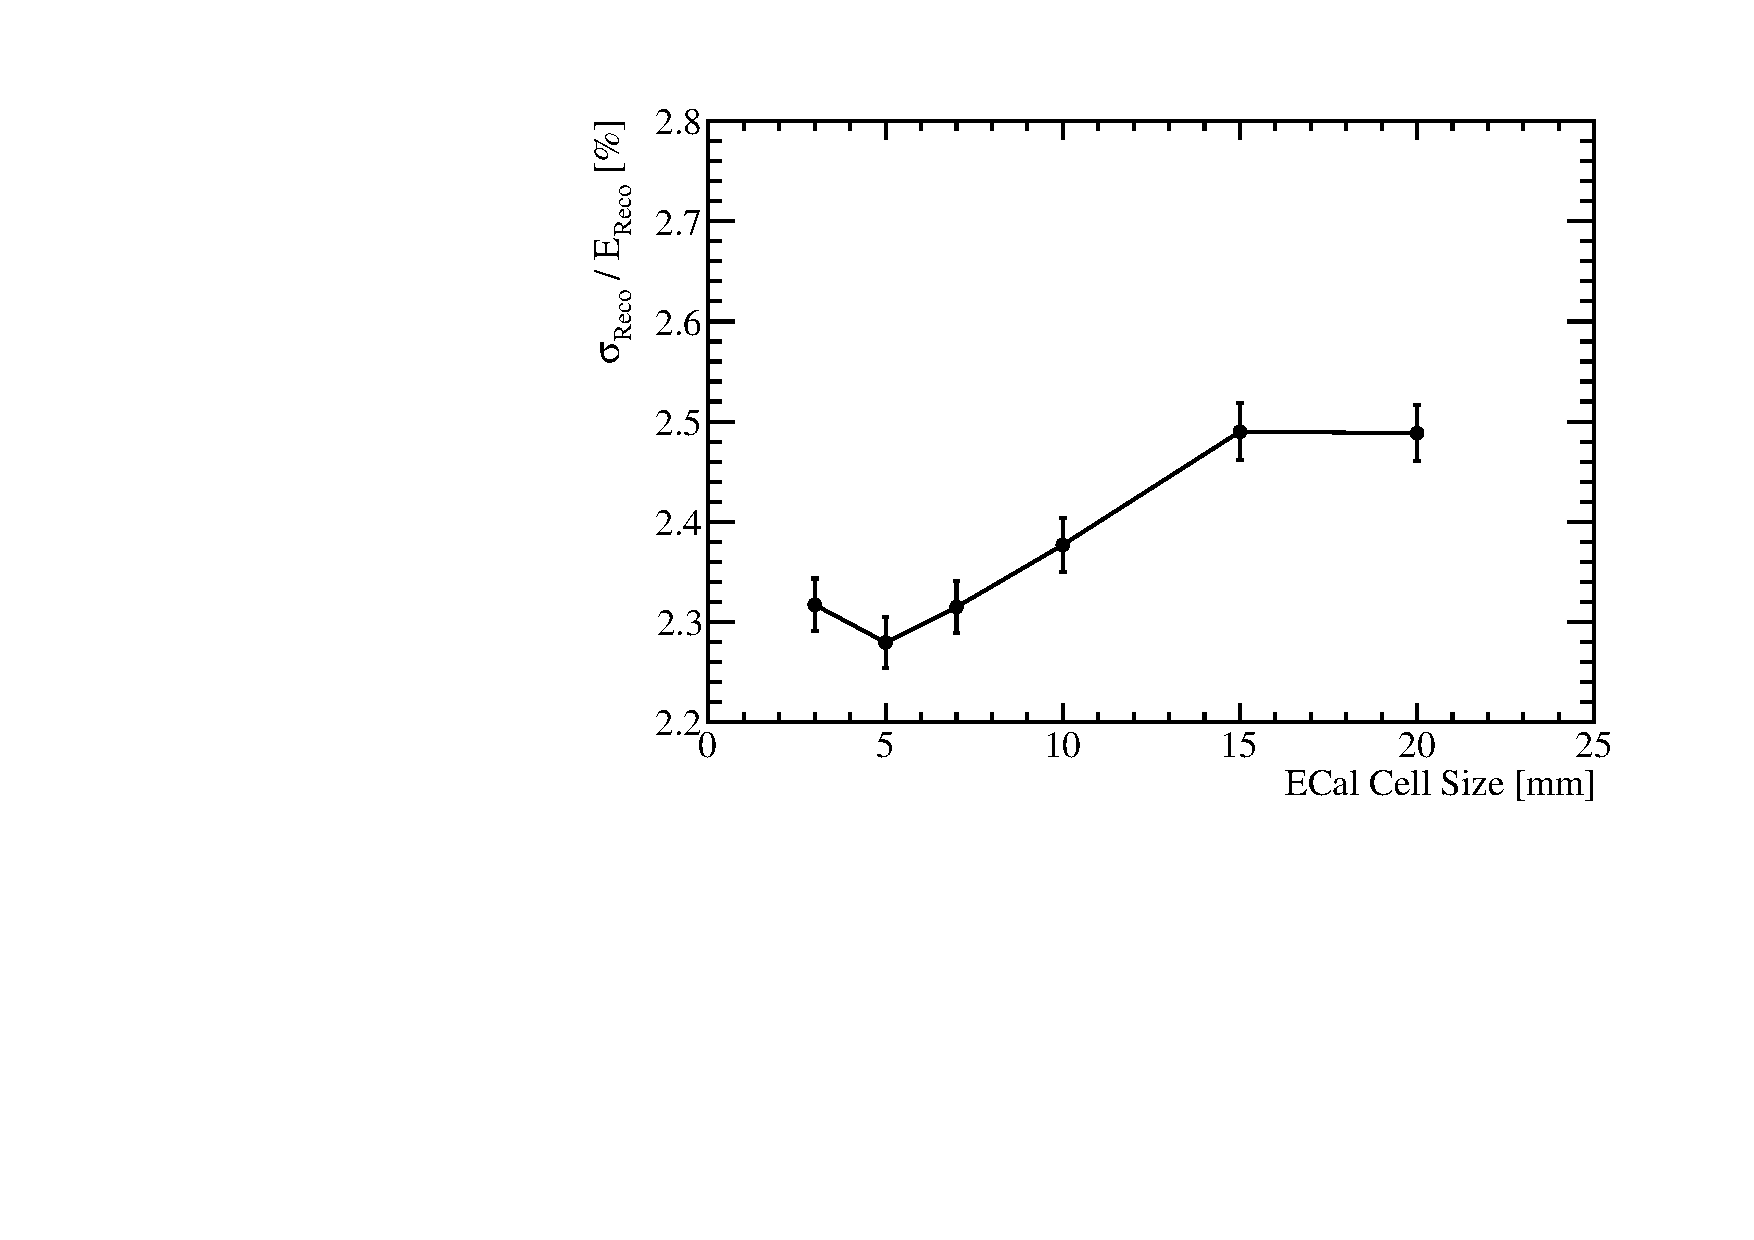
\includegraphics[width=0.5\textwidth]{OptimisationStudies/Plots/EnergyResolution/ER_vs_SiECalCellSize_100GeVPhoton.pdf}}
\subfloat[]{\label{fig:ecalsccellsize100gamma}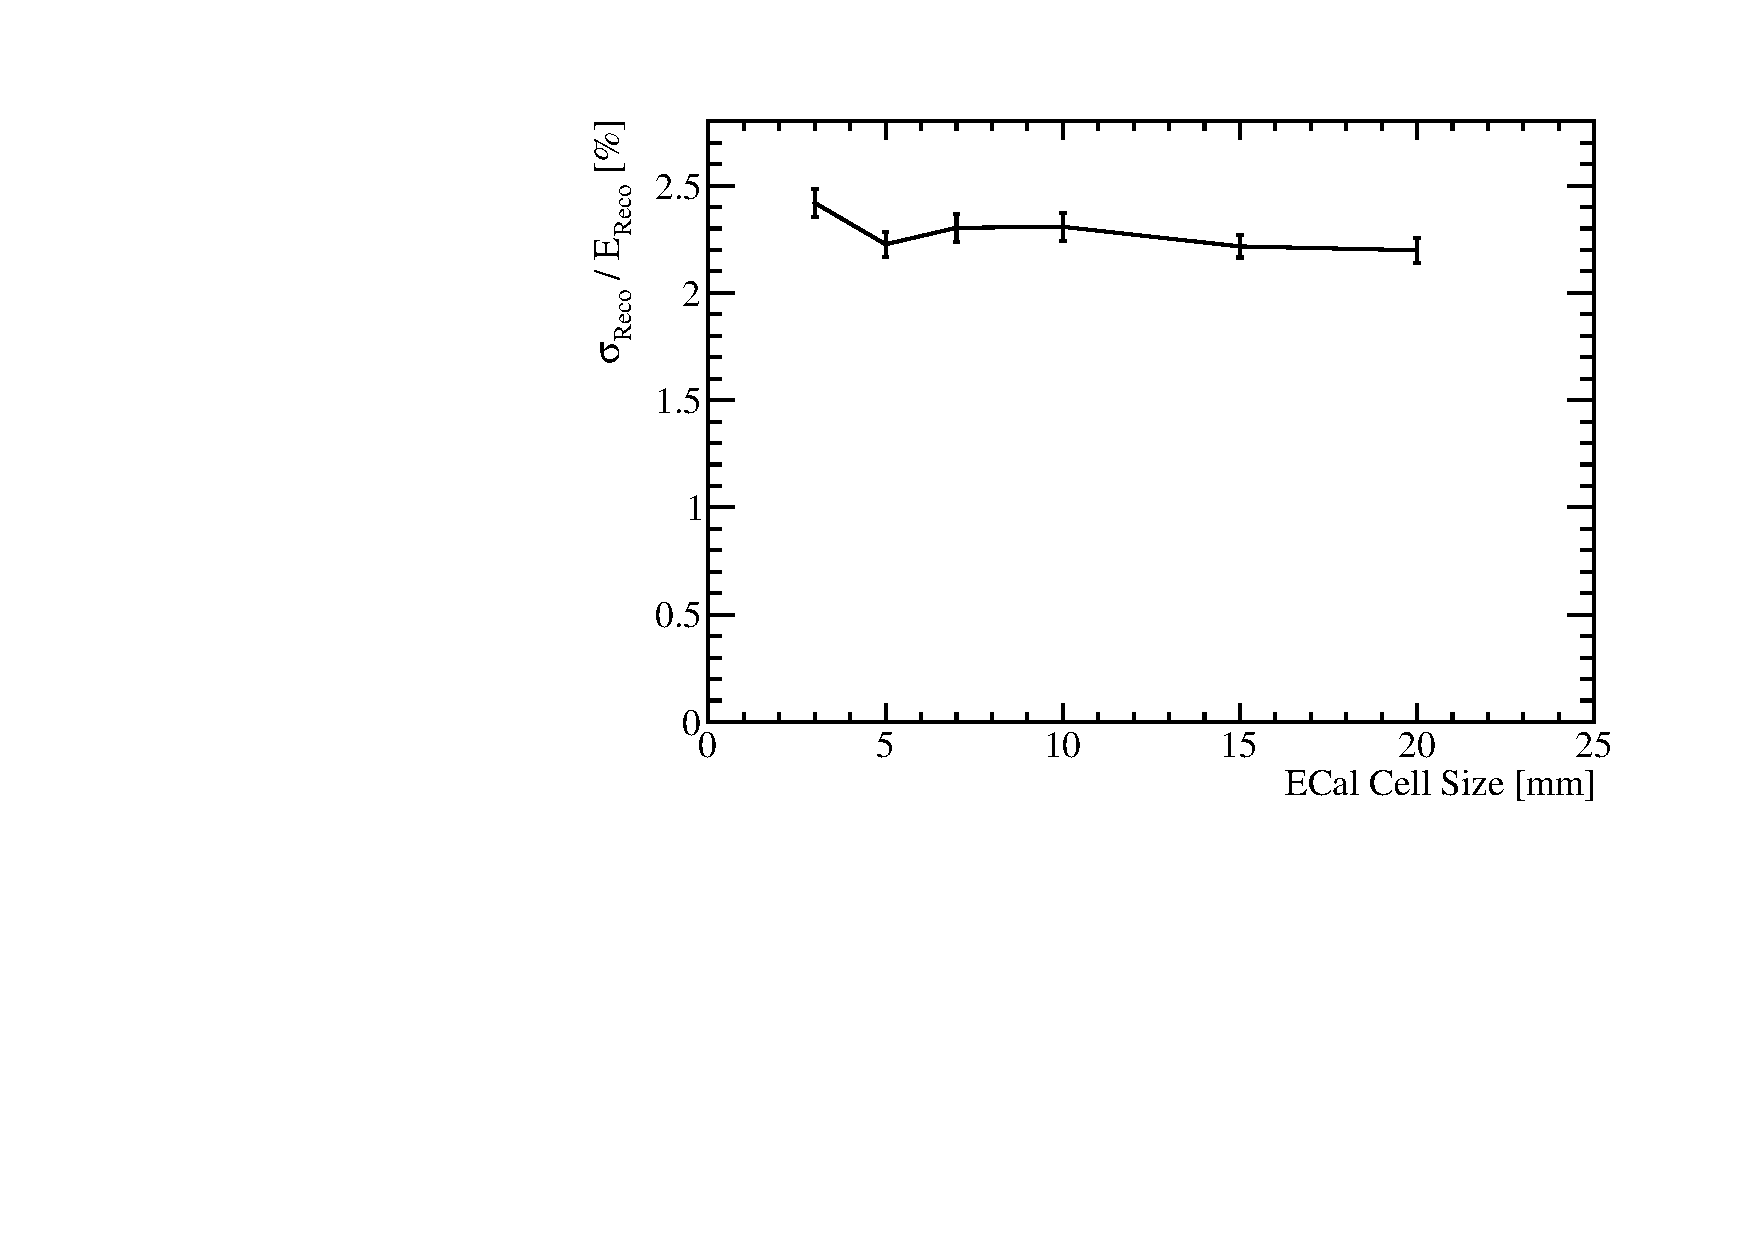
\includegraphics[width=0.5\textwidth]{OptimisationStudies/Plots/EnergyResolution/ER_vs_ScECalCellSize_100GeVPhoton.pdf}}
\caption[The energy resolution as a function of ECal cell size for 100 GeV $\gamma$s using the nominal ILD detector model with \protect\subref{fig:ecalsicellsize100gamma} the silicon and \protect\subref{fig:ecalsccellsize100gamma} the scintillator ECal option.]{The energy resolution as a function of ECal cell size for 100 GeV $\gamma$s using the nominal ILD detector model with \protect\subref{fig:ecalsicellsize100gamma} the silicon and \protect\subref{fig:ecalsccellsize100gamma} the scintillator ECal option.}
\label{fig:ecalcellsizegamma}
\end{figure}

The energy resolution, using 100 GeV $\gamma$ events, as a function of the ECal cell size is shown in figure \ref{fig:ecalsicellsize} for the silicon option and figure \ref{fig:ecalsccellsize} for the scintillator option.  As at these energies the $\gamma$ will be largely contained within the ECal these results relate solely to the energy resolution of the ECal within the full ILD simulation.  For both the silicon and scintillator ECal options the energy resolution does not depend strongly on the ECal cell size.  This is to be expected as the sampling frequency, which is the main factor in determining the energy resolution of a calorimeter, does not change when modifying the cell size.  There are minor fluctuations in the energy resolution when varying the cell size, but these are mostly likely due to fluctuations in the energy response from calibration procedure that was applied to each detector models.  For the scintillator ECal option there is a significant degradation in the energy resolution for the $3 \times 3 \text{mm}^{2}$ cell size model.  The most likely cause of this is a "dead" region in the active material, which represents the readout multi pixel photon counter (MPPC).  The MPPC occupies a fixed area of the cell irrespective of cell size and so fractionally the dead region of the cell increases as cell size is reduced (CITE).  The larger this dead region the worse the sampling of the electromagnetic showers in the ECal and the worse the resolution.  While this effect will be present in all scintillator ECal options, it will only be significant for the small cell sizes when fractionally the dead region is largest.  This would explain why the degradation is only seen at the smallest cell size considered.     

The separation of nearby particle showers within the calorimeter is limited by the cell size.  Smaller cell size make it easier separate nearby particle showers, which causes a reduction in the track to calorimeter cluster association confusion.  Therefore, although the intrinsic energy resolution of a calorimeter is not dependent on the cell size it is expected that the jet energy resolution be far more sensitive to the ECal cell size.  The jet energy resolution as a function of ECal cell size is shown in figure \ref{fig:ecalsicellsize} for the silicon option and figure \ref{fig:ecalsccellsize} for the scintillator option.  As expected there is a very strong dependancy on the ECal cell size with smaller cell sizes leading to lower values of the jet energy resolution.  The origin of this trend is best illustrated by considering the intrinsic energy resolution and confusion contributions to the jet energy resolution, which are shown as a function of ECal cell size for 45 and 250 GeV jets, for both the silicon and scintillator ECal options, in figure \ref{fig:ecalcellsizebreak}.  It is clear from these contributions that the intrinsic energy resolution of the detector does not change when varying the cell size, which agrees with both prior expectations of calorimeter behaviour and the single particle energy resolution study.  The minor fluctuations seen in the energy resolution for the single particle study are washed out when considering the intrinsic energy resolution for jets, as only $~30\%$ of jet energy is carried in the form of $\gamma$s.  Furthermore, the jet energy resolution trend as a function of the ECal cell size is being driven purely by changes to the confusion contribution and, in particular, the confusion caused by the reconstruction of $\gamma$s.  This is exactly what is to expected given the ECal primarily measures $\gamma$s and shows that the performance of the ECal when varying the cell size is well understood.

It is clear that the ECal cell size is extremely important for the jet energy resolution of the detector, but it has little bearing on the intrinsic energy resolution.  To ensure separation of hadronic decays of W and Z bosons is possible at ILC like energies an ECal cell size of least $15 \times 15 \text{mm}^{2}$ is crucial, however, as reducing the ECal cell size further continues to improve the jet energy resolution choosing the smallest size possible is desirable.   

% JER
\begin{figure}
\centering
\subfloat[]{\label{fig:ecalsicellsize}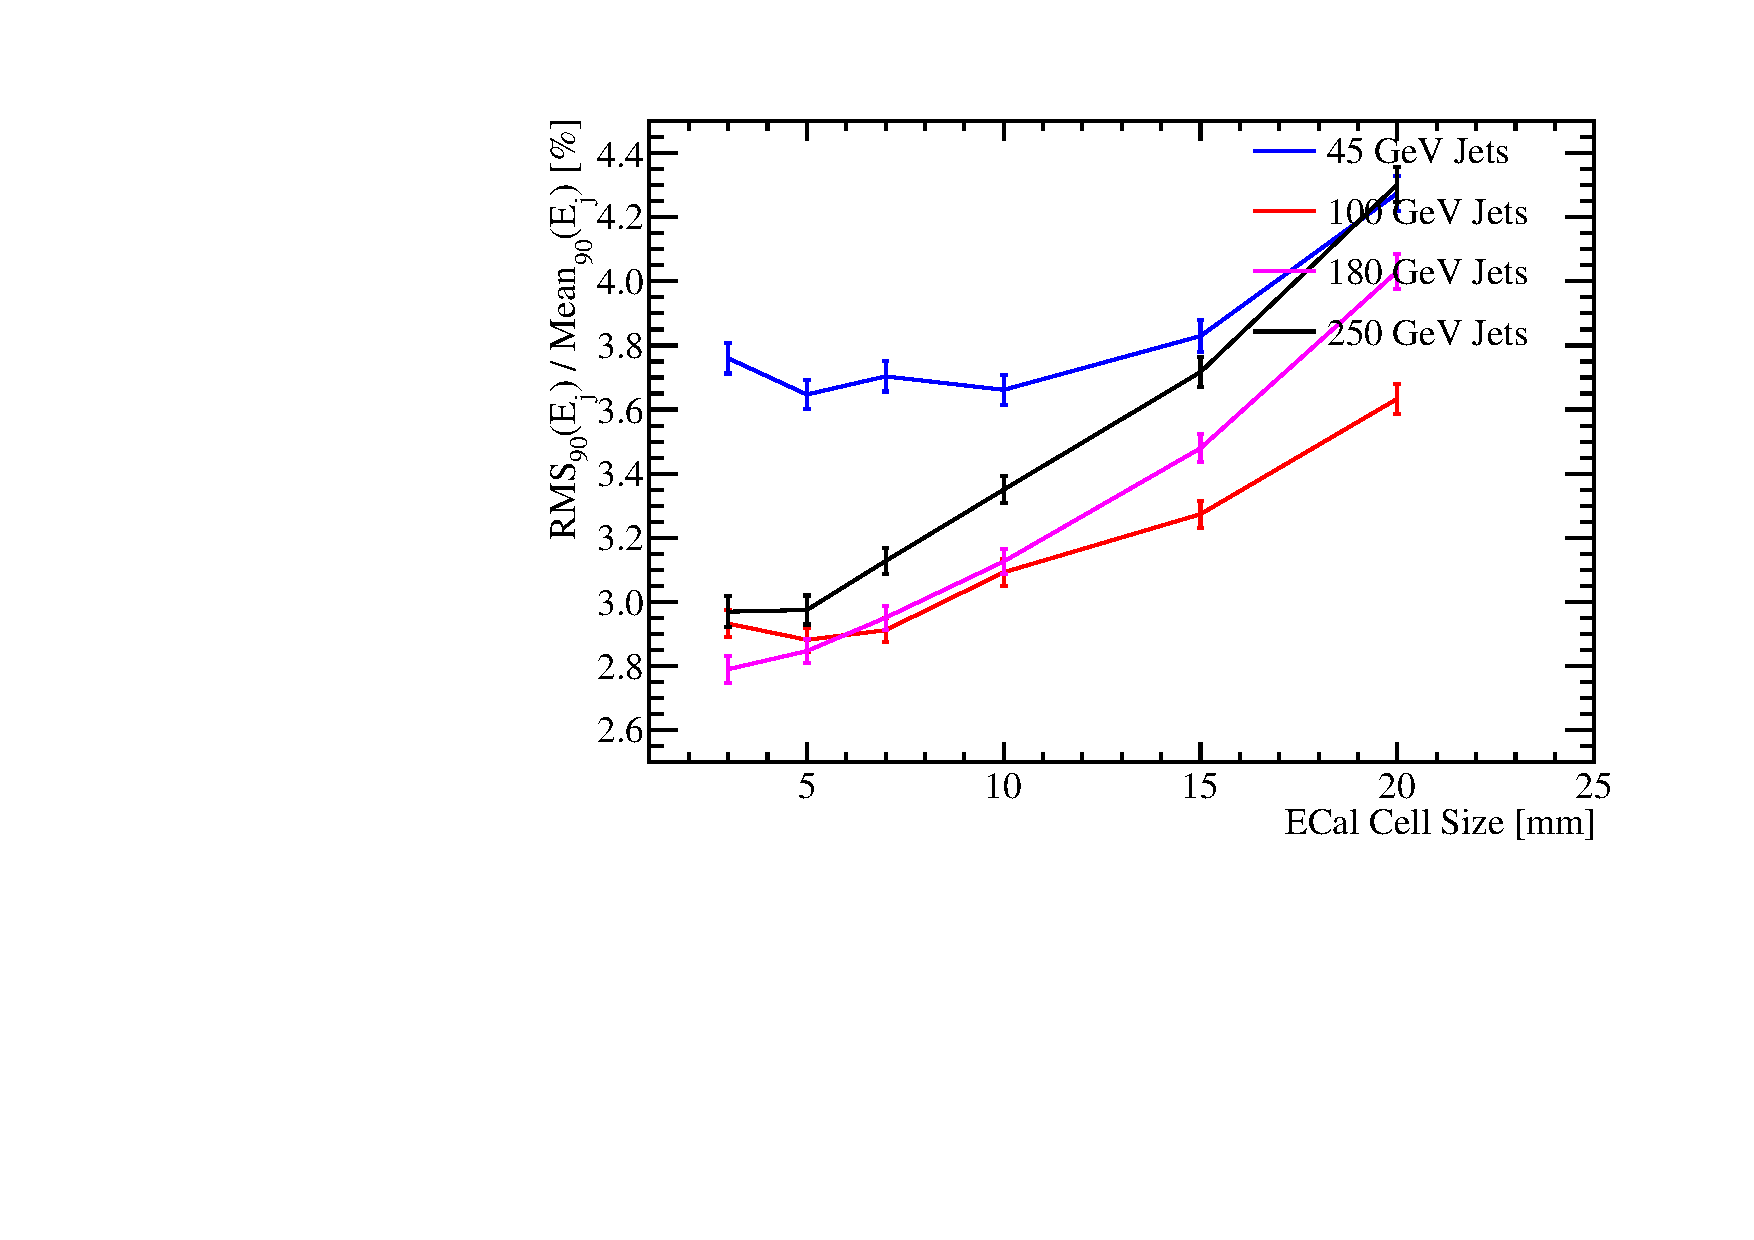
\includegraphics[width=0.5\textwidth]{OptimisationStudies/Plots/JetEnergyResolutions/JER_vs_SiliconECalCellSize.pdf}}
\subfloat[]{\label{fig:ecalsccellsize}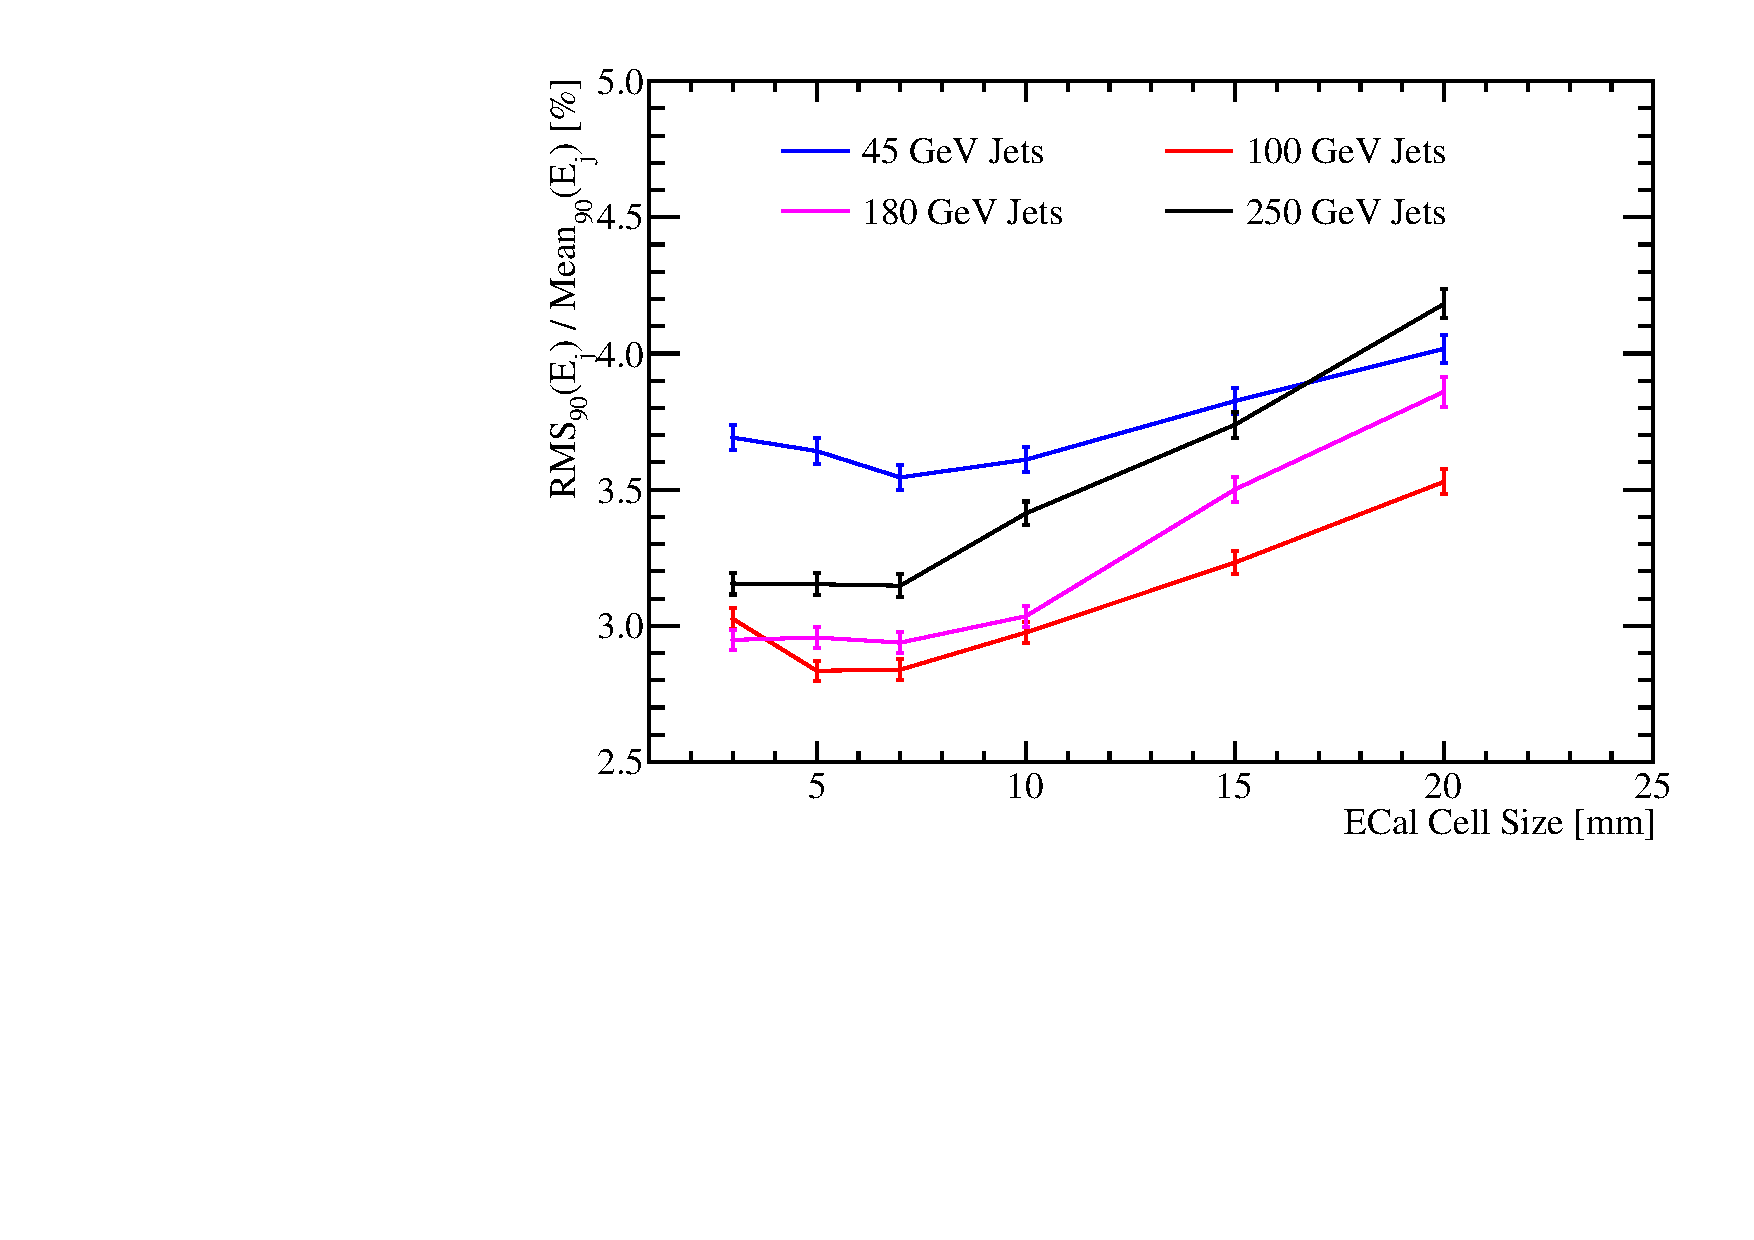
\includegraphics[width=0.5\textwidth]{OptimisationStudies/Plots/JetEnergyResolutions/JER_vs_ScintillatorECalCellSize.pdf}} \hfill
\caption[The jet energy resolution as a function of ECal cell size for various jet energies using the nominal ILD detector model with \protect\subref{fig:ecalsicellsize} the silicon and \protect\subref{fig:ecalsccellsize} the scintillator ECal option.]{The jet energy resolution as a function of ECal cell size for various jet energies using the nominal ILD detector model with \protect\subref{fig:ecalsicellsize} the silicon and \protect\subref{fig:ecalsccellsize} the scintillator ECal option.}
\label{fig:ecalcellsize}
\end{figure}

% JER BD
\begin{figure}
\centering
\subfloat[]{\label{fig:ecalsicellsize45break}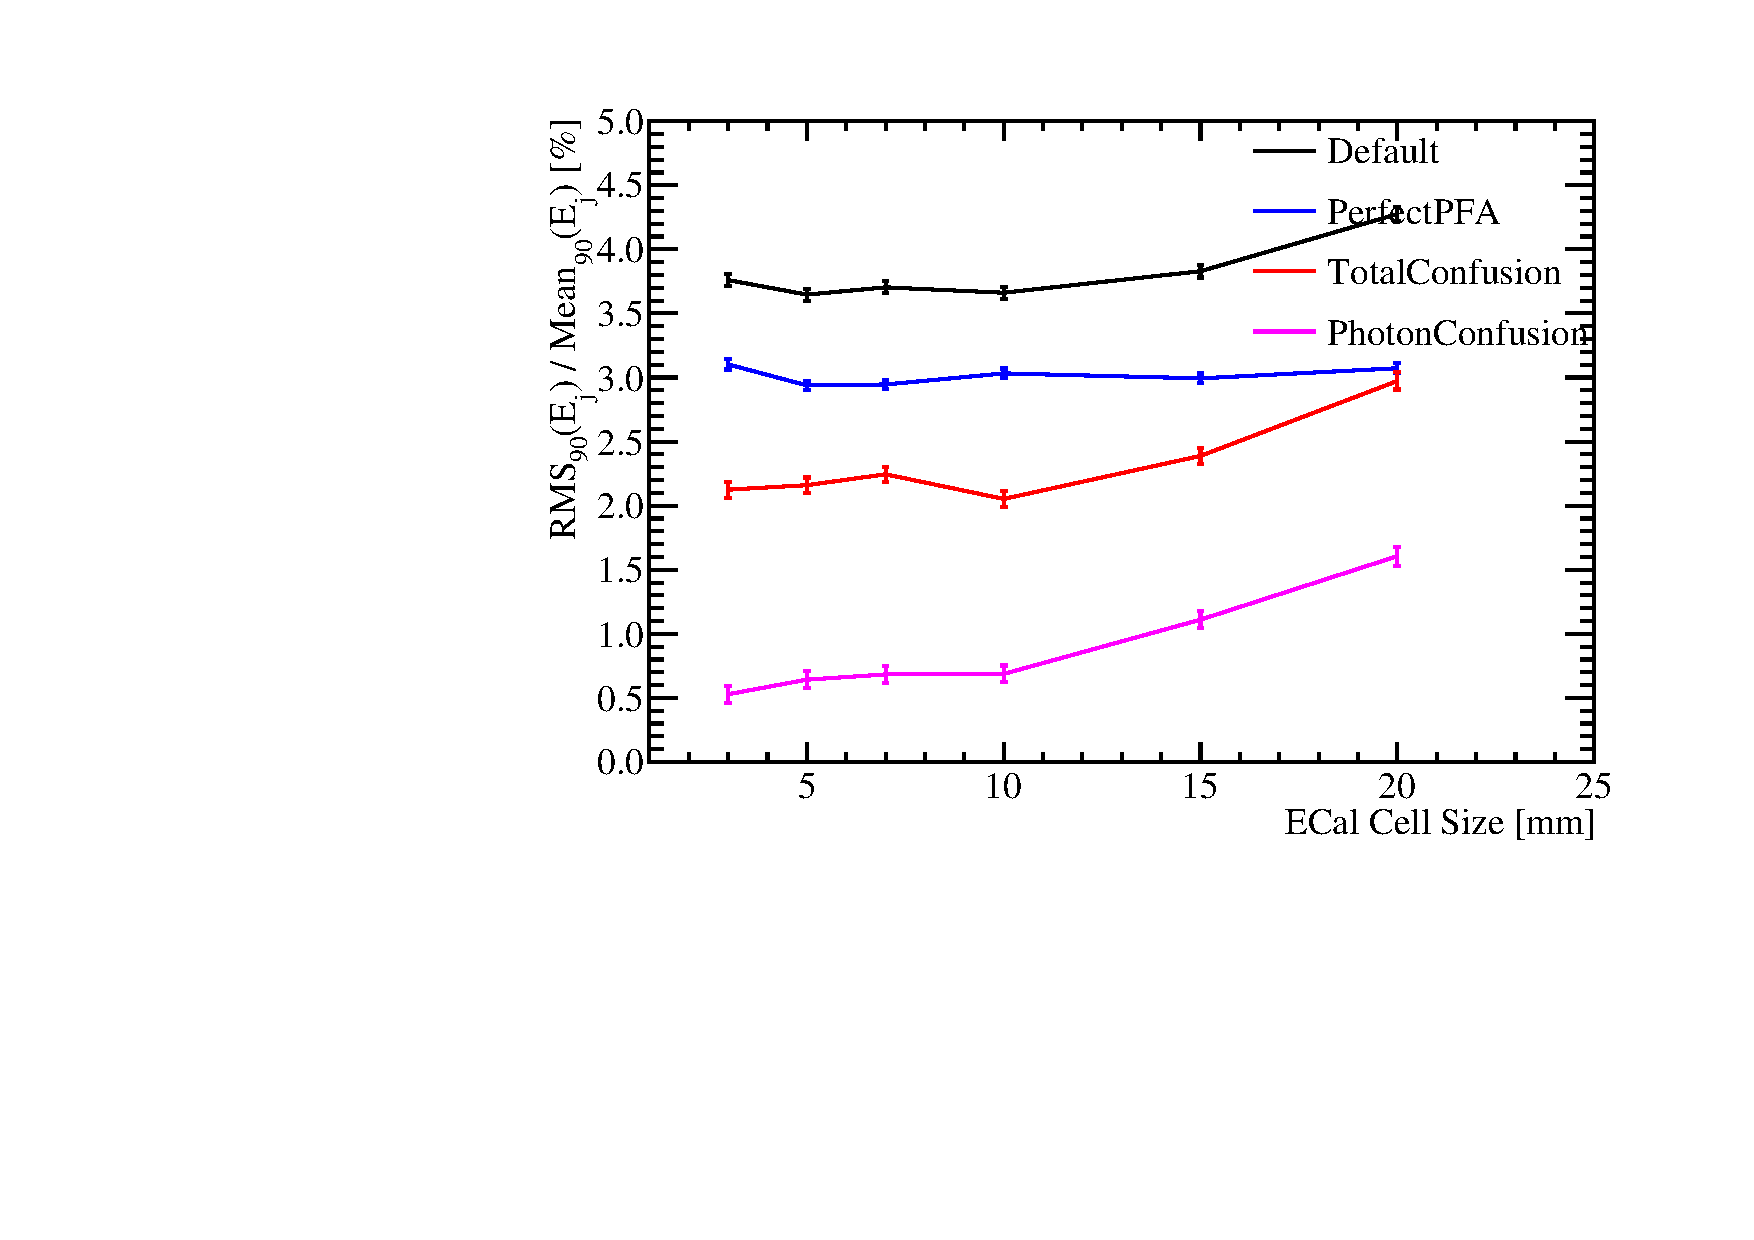
\includegraphics[width=0.5\textwidth]{OptimisationStudies/Plots/JetEnergyResolutions/JER_vs_SiliconECalCellSize_91GeV_DiJet_Breakdown.pdf}}
\subfloat[]{\label{fig:ecalsccellsize45break}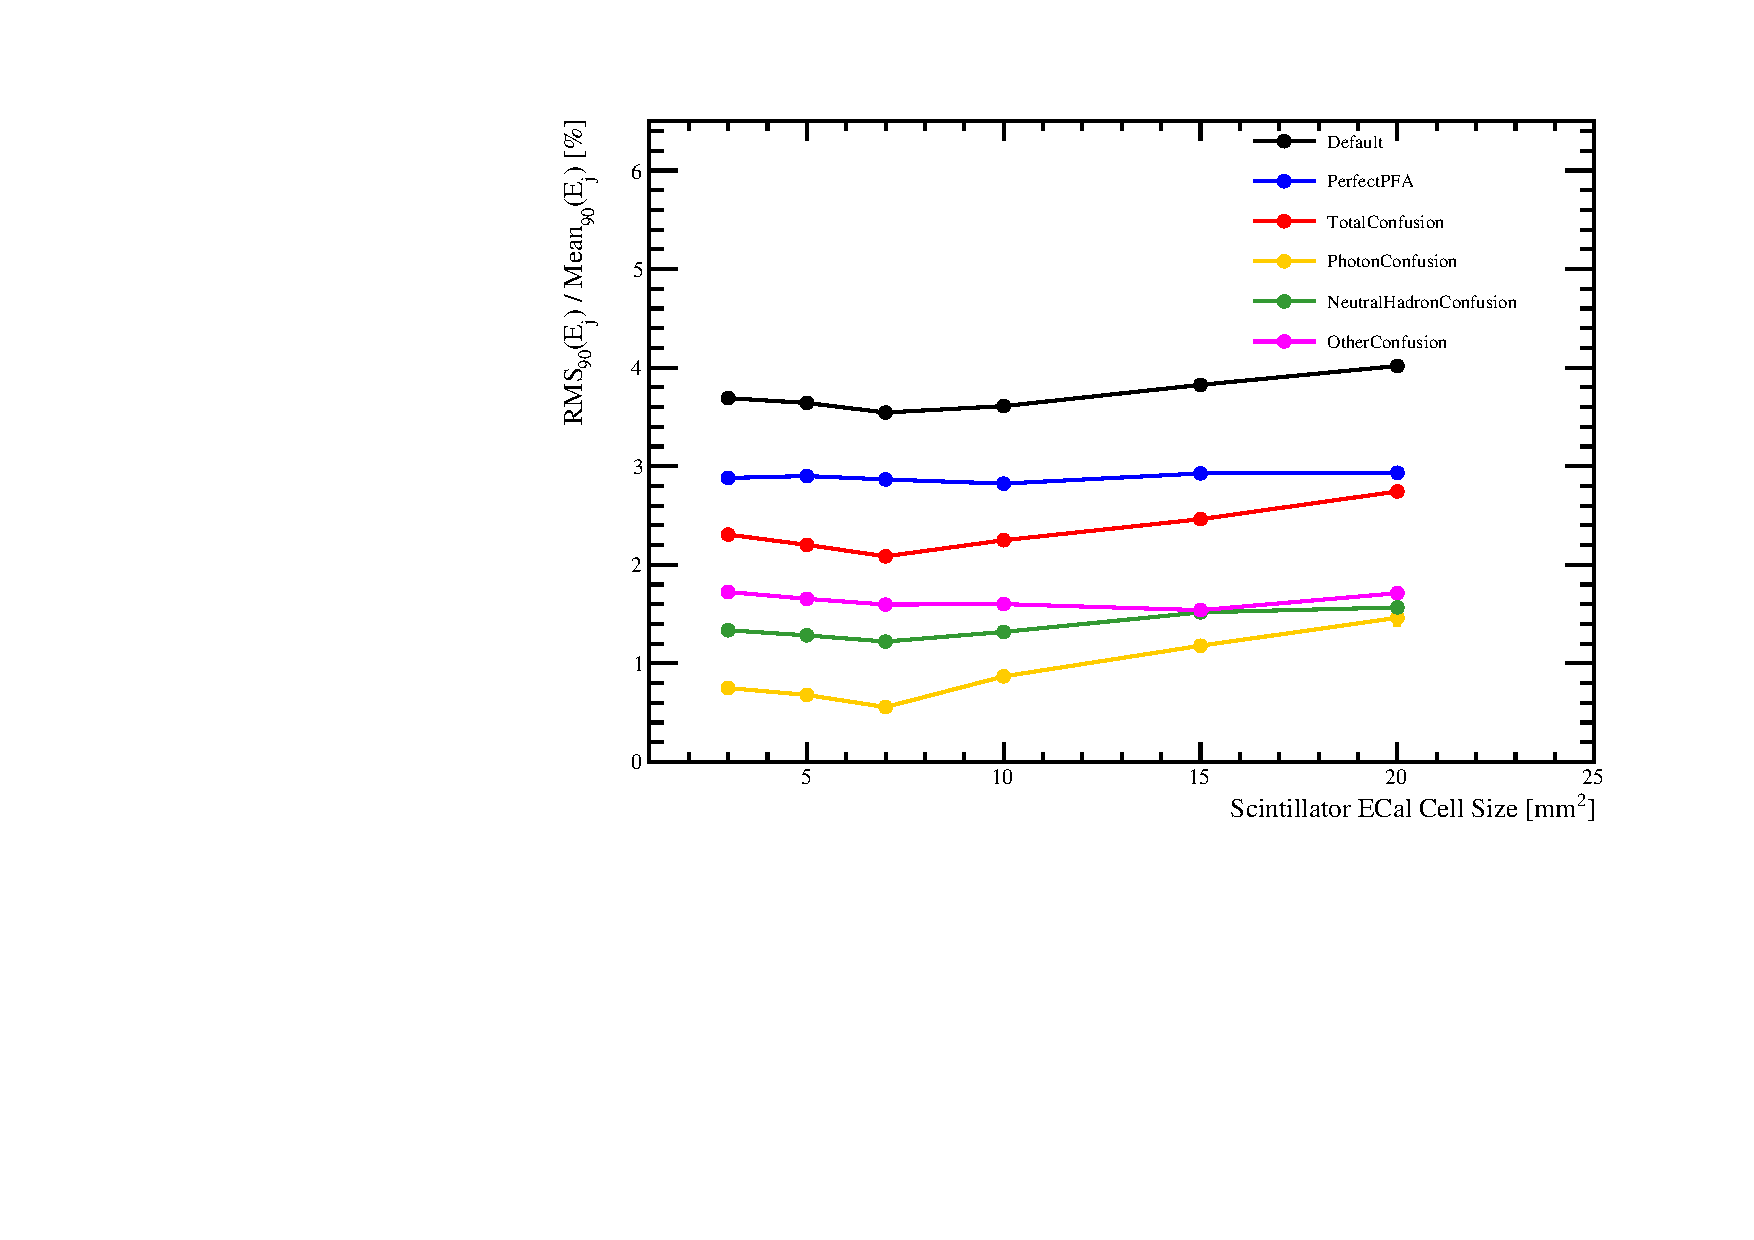
\includegraphics[width=0.5\textwidth]{OptimisationStudies/Plots/JetEnergyResolutions/JER_vs_ScintillatorECalCellSize_91GeV_DiJet_Breakdown.pdf}} \hfill
\subfloat[]{\label{fig:ecalsicellsize250break}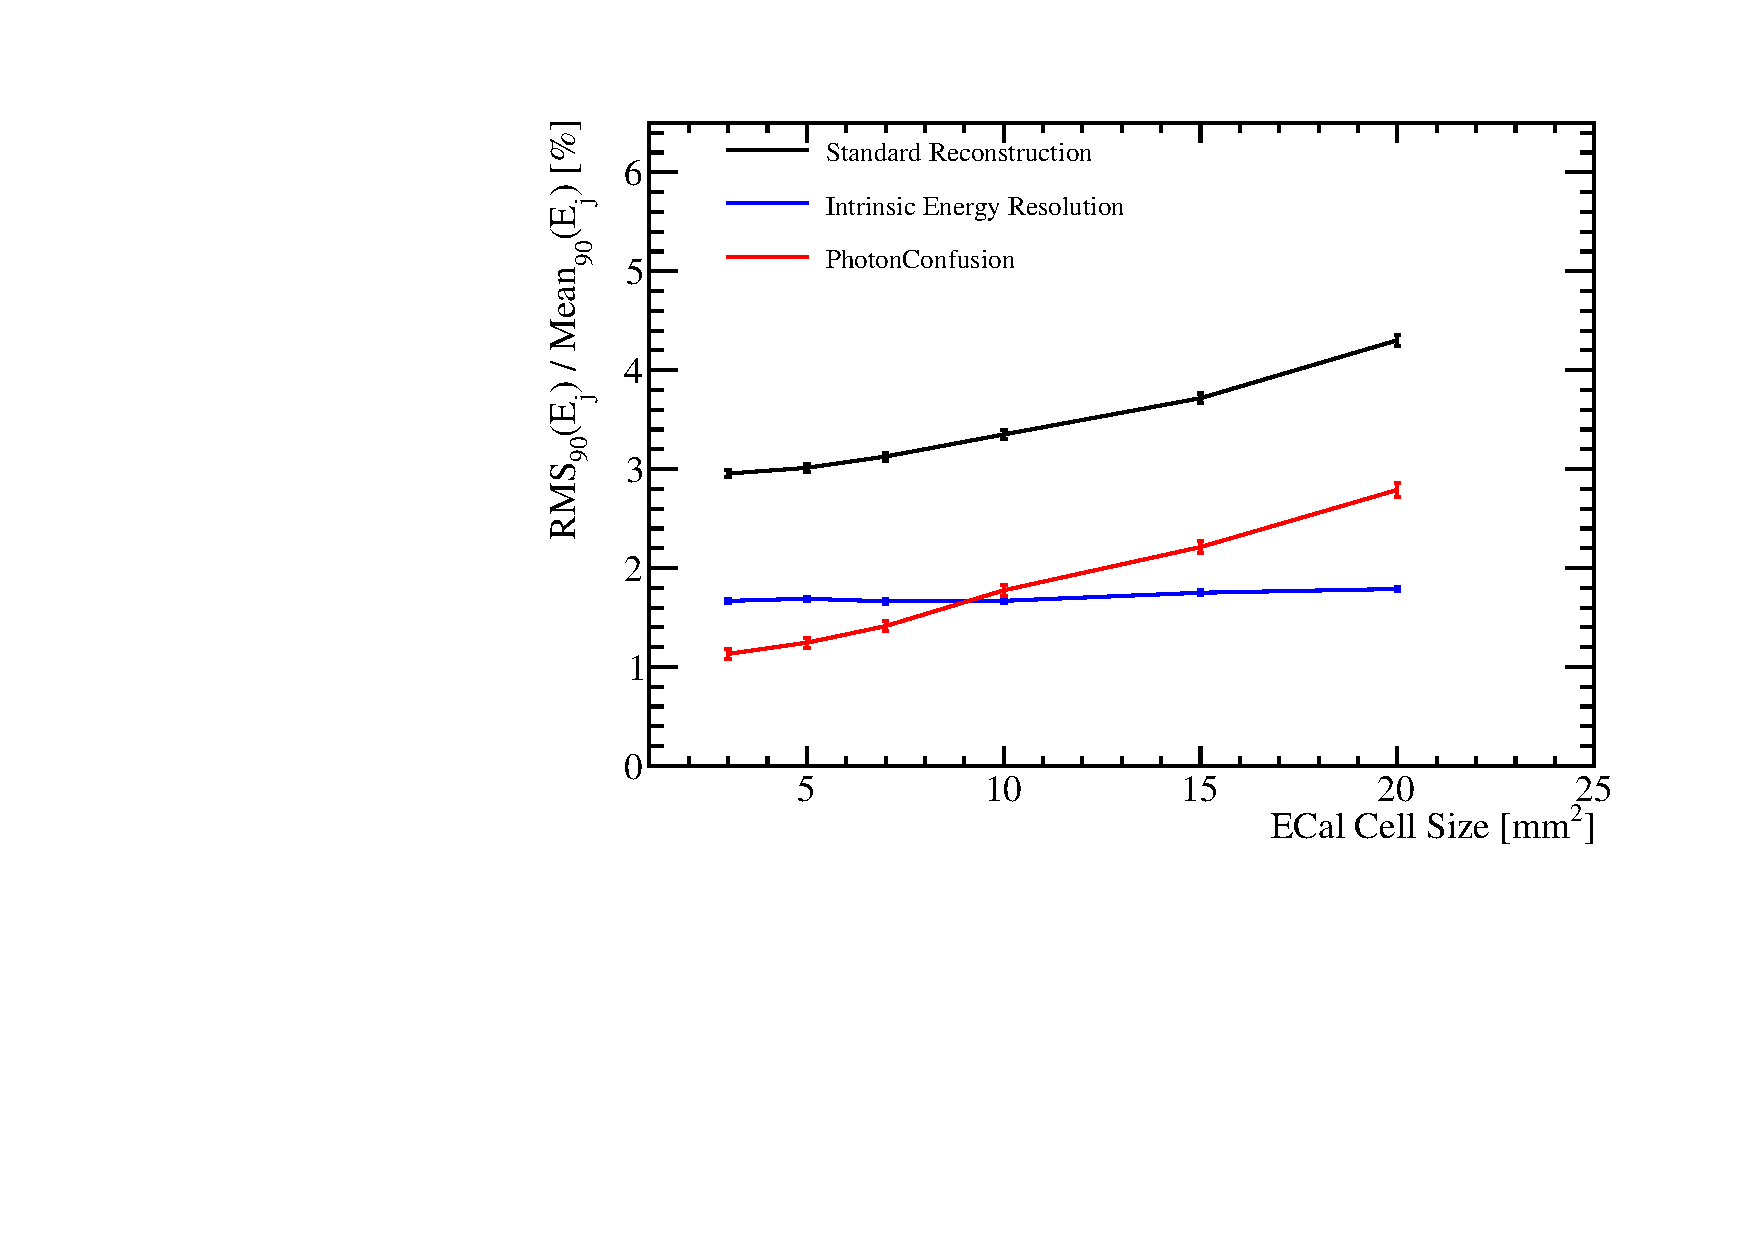
\includegraphics[width=0.5\textwidth]{OptimisationStudies/Plots/JetEnergyResolutions/JER_vs_SiliconECalCellSize_500GeV_DiJet_Breakdown.pdf}}
\subfloat[]{\label{fig:ecalsccellsize250break}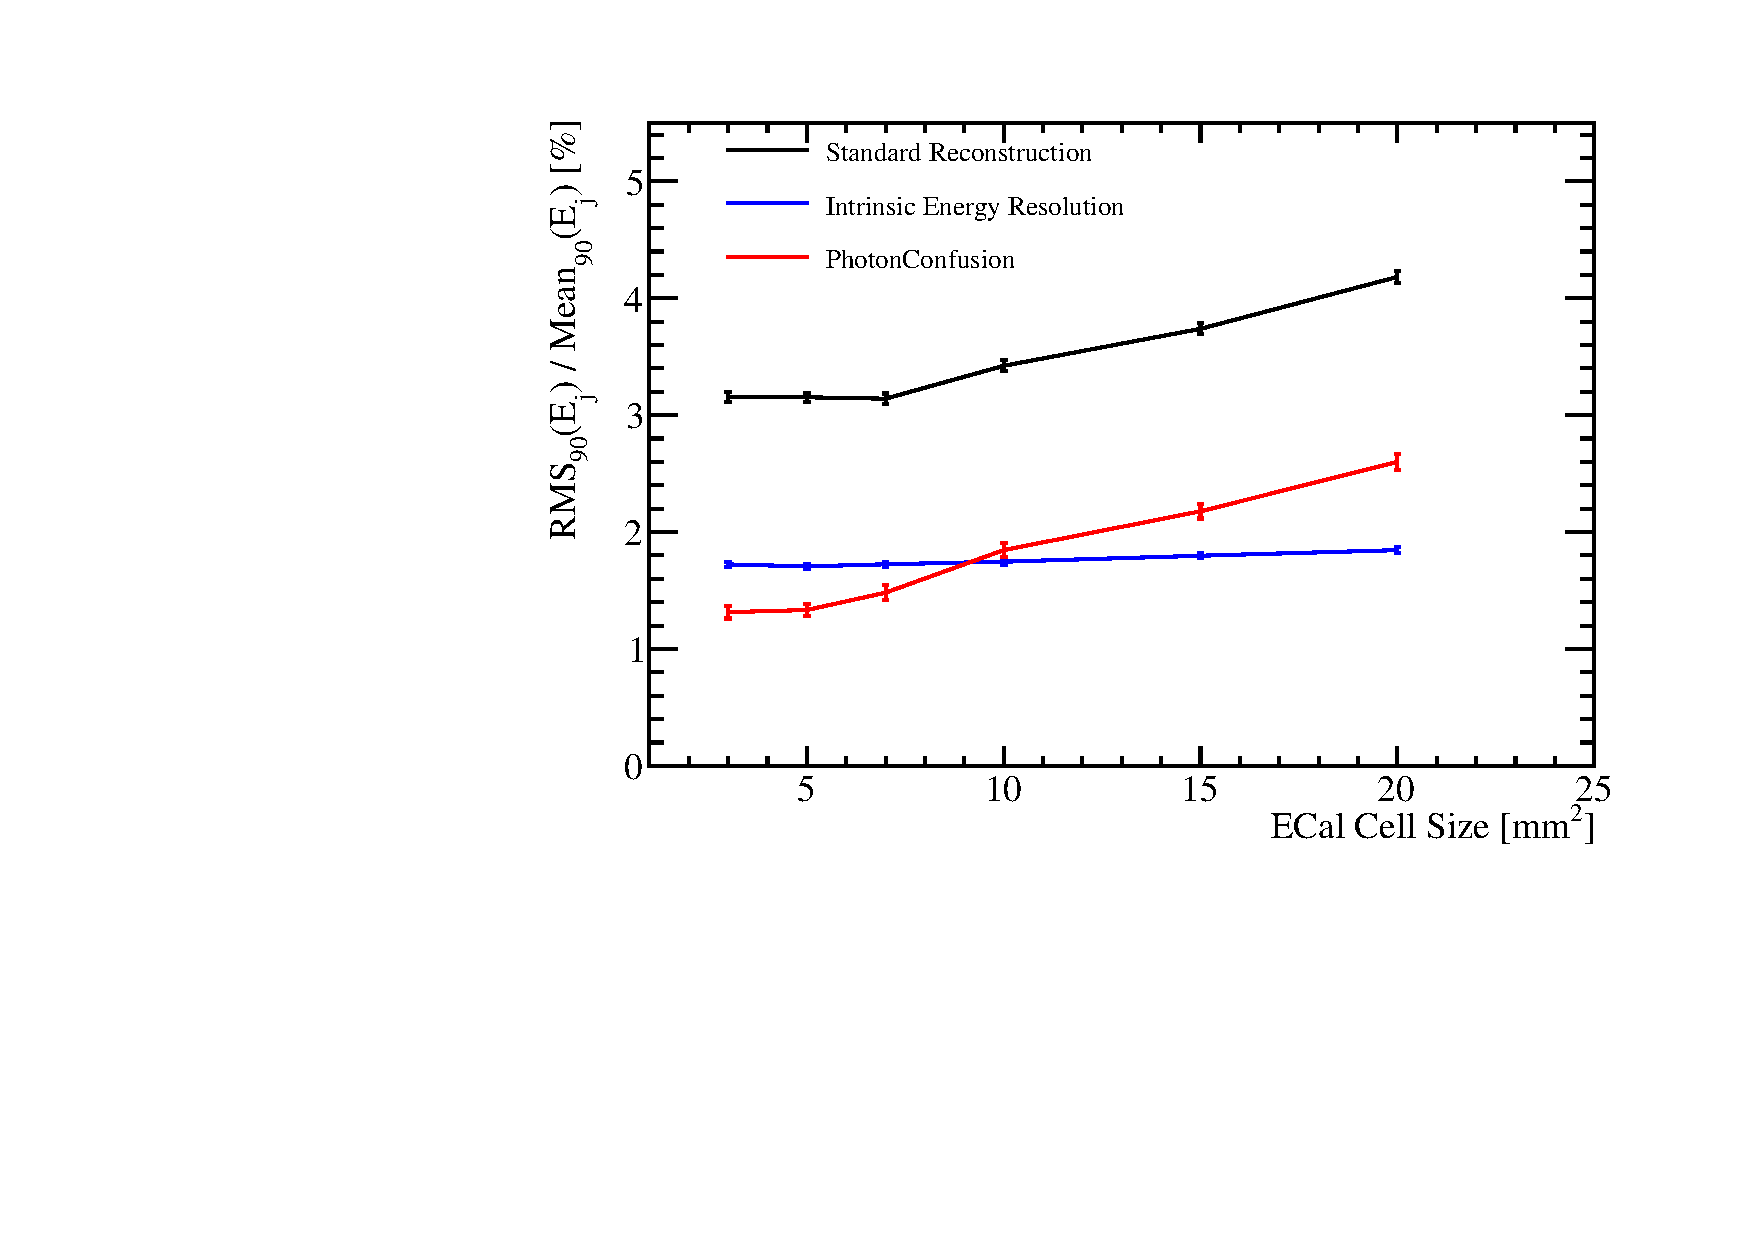
\includegraphics[width=0.5\textwidth]{OptimisationStudies/Plots/JetEnergyResolutions/JER_vs_ScintillatorECalCellSize_500GeV_DiJet_Breakdown.pdf}}
\caption[The contributions to the jet energy resolution as a function of ECal cell size using the nominal ILD detector model for \protect\subref{fig:ecalsicellsize45break} the silicon ECal option and 45 GeV jets, \protect\subref{fig:ecalsccellsize45break} the scintillator ECal option and 45 GeV jets, \protect\subref{fig:ecalsicellsize250break} the silicon ECal option and 250 GeV jets and \protect\subref{fig:ecalsccellsize250break} the scintillator ECal option and 250 GeV jets.  The black curve correspond to the standard reconstruction, the blue curve to the intrinsic energy resolution contribution to the jet energy resolution, the red curve to the confusion contribution to the jet energy resolution and the magenta curve to the confusion contribution to the jet energy resolution related solely to $\gamma$ reconstruction.]{The contributions to the jet energy resolution as a function of ECal cell size using the nominal ILD detector model for \protect\subref{fig:ecalsicellsize45break} the silicon ECal option and 45 GeV jets, \protect\subref{fig:ecalsccellsize45break} the scintillator ECal option and 45 GeV jets, \protect\subref{fig:ecalsicellsize250break} the silicon ECal option and 250 GeV jets and \protect\subref{fig:ecalsccellsize250break} the scintillator ECal option and 250 GeV jets.  The black curve correspond to the standard reconstruction, the blue curve to the intrinsic energy resolution contribution to the jet energy resolution, the red curve to the confusion contribution to the jet energy resolution and the magenta curve to the confusion contribution to the jet energy resolution related solely to $\gamma$ reconstruction}
\label{fig:ecalcellsizebreak}
\end{figure}

%========================================================================================

\subsection{ECal Number of Layers}
\label{sec:ecalnlayers}
The ECal performance was simulated for different numbers of sampling layers, while keeping the total material budget ($\text{X}_{0}$) approximately constant.  This study was performed for both the silicon and scintillator active material options.  In all cases tungsten was used for the ECal absorber material and the active layer thicknesses were not changed from those used in the nominal ECal models found in table \ref{table:defaultildecal}.  The different layouts for the ECals considered here are summarised in table \ref{table:nlayersecaloption}.  

\begin{table}[h!]
\centering
\begin{tabular}{ l l l l l l}
\hline
Total Number & $N_{Layers}$ & Absorber & $N_{Layers}$ & Absorber & Total  \\
of Layers & Region 1 & Thickness & Region 2 & Thickness & Thickness \\
$N_{\text{Layers ECal}}$ & & Region 1 [mm] & &  Region 2 [mm] &  [$\text{X}_{0}$] \\
\hline
30 & 20 & 2.10 & 9 & 4.20 & 22.77 \\
26 & 17 & 2.40 & 8 & 4.80 & 22.60 \\
20 & 13 & 3.15 & 6 & 6.30 & 22.47 \\
16 & 10 & 4.00 & 5 & 8.00 & 22.31\\
\hline
\end{tabular}
\caption[The longitudinal structure of the ECal models considered in the optimisation study.  The radiation length of tungsten absorber is 3.504mm \cite{Olive:2016xmw}.  Note that a presampler layer contributes one extra layer to the cumulative number of layers value for all detector models considered.]{The longitudinal structure of the ECal models considered in the optimisation study.  The radiation length of tungsten absorber is 3.504mm \cite{Olive:2016xmw}.  Note that a presampler layer contributes one extra layer to the cumulative number of layers value for all detector models considered.}
\label{table:nlayersecaloption}
\end{table}

% SP
\begin{figure}
\centering
\subfloat[]{\label{fig:ecalsinlayers100gamma}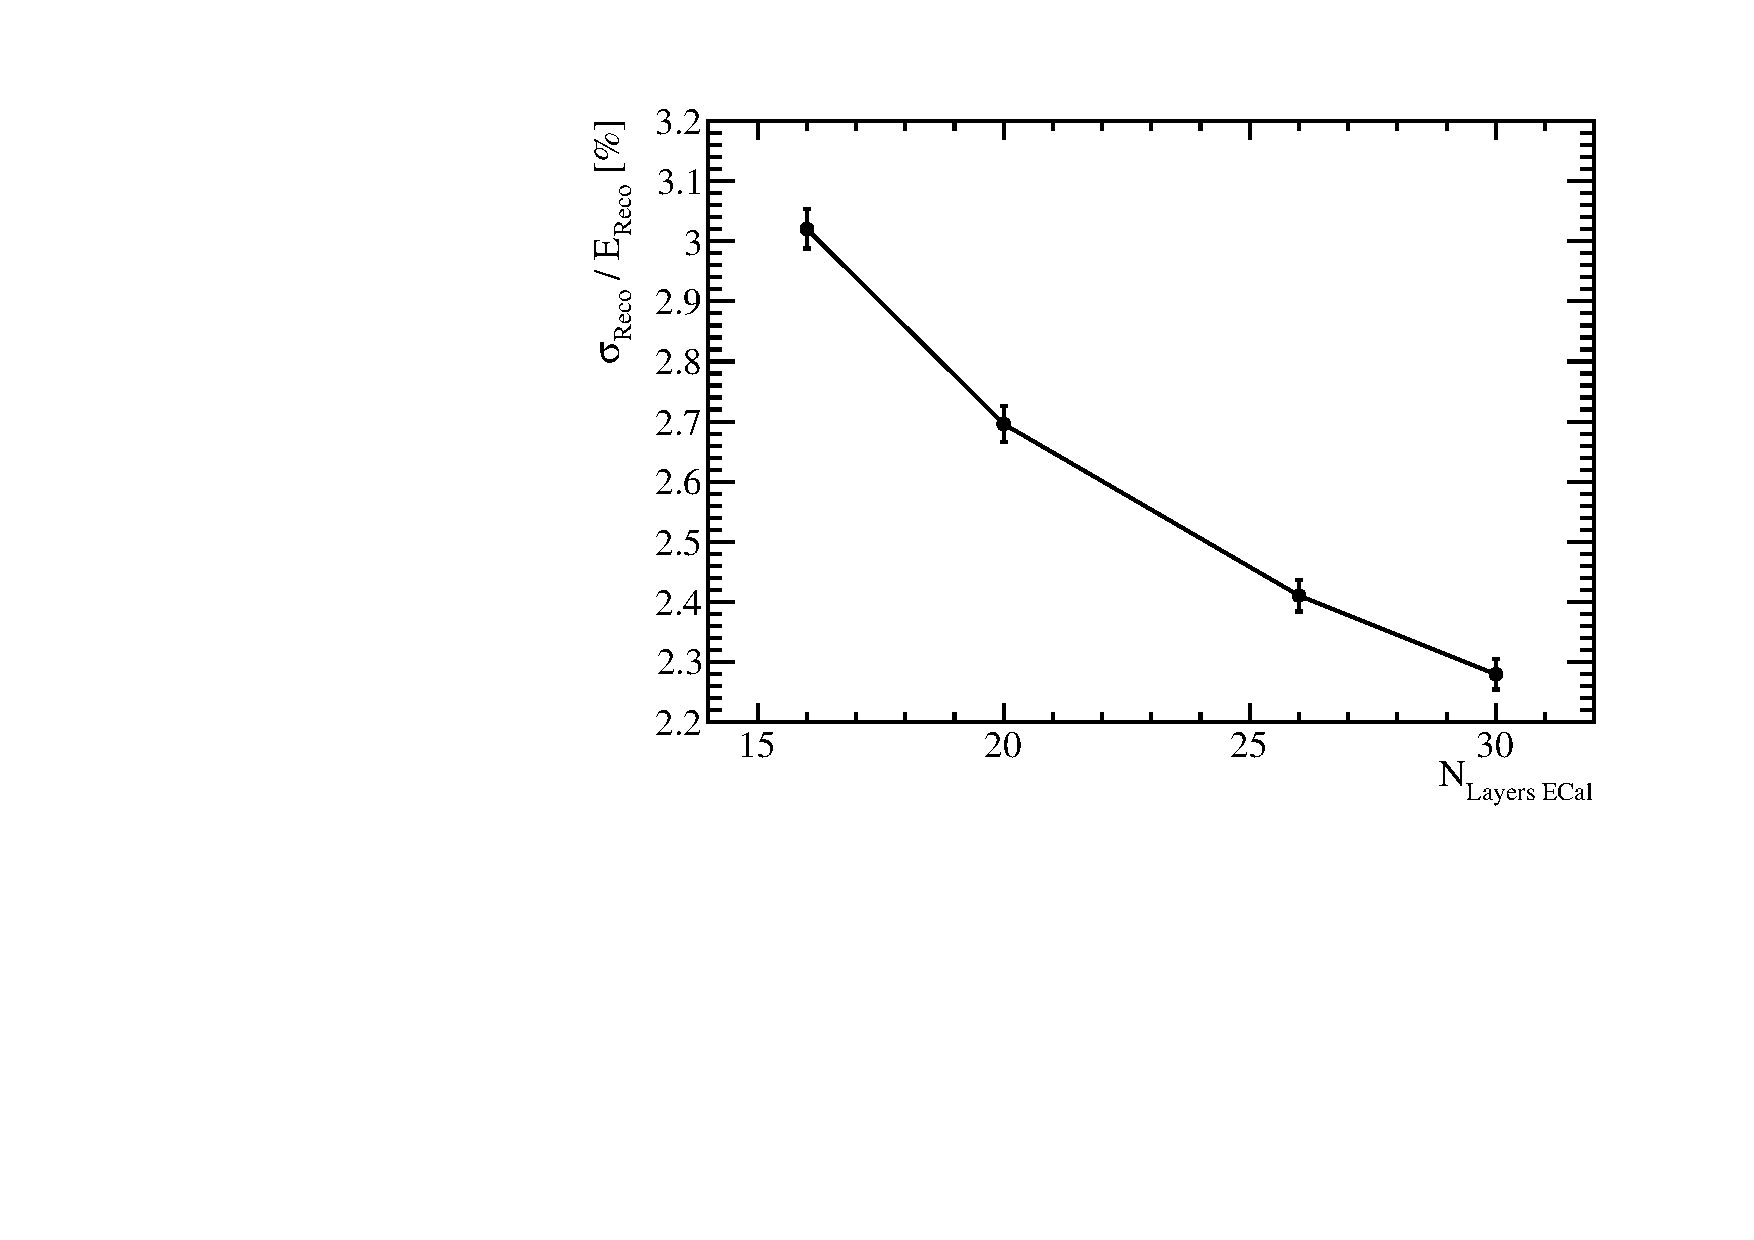
\includegraphics[width=0.5\textwidth]{OptimisationStudies/Plots/EnergyResolution/ER_vs_SiECalNLayers_100GeVPhoton.pdf}}
\subfloat[]{\label{fig:ecalscnlayers100gamma}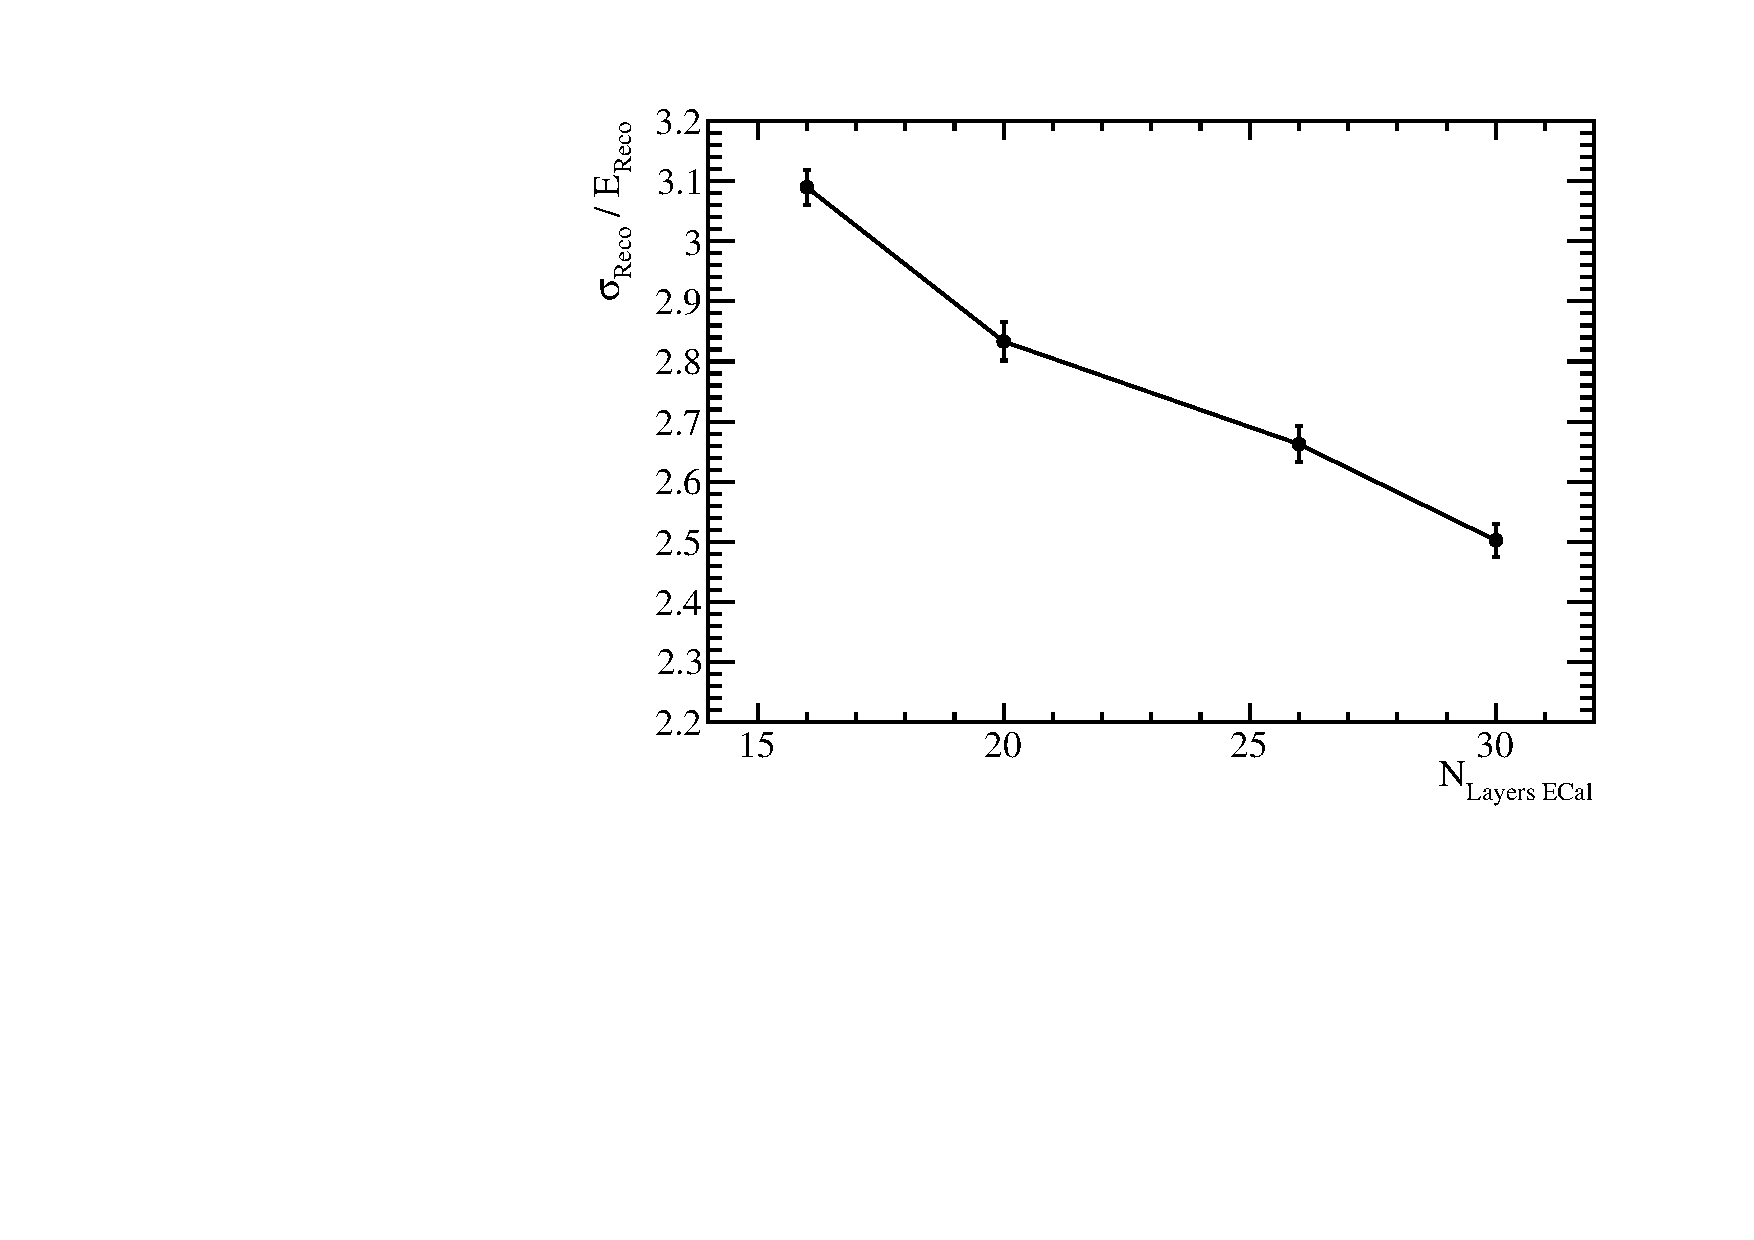
\includegraphics[width=0.5\textwidth]{OptimisationStudies/Plots/EnergyResolution/ER_vs_ScECalNLayers_100GeVPhoton.pdf}}
\caption[The energy resolution as a function of number of layers in the ECal for 100 GeV $\gamma$s using the nominal ILD detector model with \protect\subref{fig:ecalsinlayers100gamma} the silicon and \protect\subref{fig:ecalscnlayers100gamma} the scintillator ECal option.]{The energy resolution as a function of number of layers in the ECal for 100 GeV $\gamma$s using the nominal ILD detector model with \protect\subref{fig:ecalsinlayers100gamma} the silicon and \protect\subref{fig:ecalscnlayers100gamma} the scintillator ECal option.}
\label{fig:ecalnlayersgamma}
\end{figure}

The energy resolution, using 100 GeV $\gamma$ events, as a function of the number of layers in the ECal is shown in figure \ref{fig:ecalsinlayers100gamma} for the silicon option and figure \ref{fig:ecalscnlayers100gamma} for the scintillator option.  As the number of layers is reduced the energy resolution increases, which is expected as more layers means greater the sampling of the electromagnetic particle showers and a reduction in the stochastic contribution to the energy resolution.  The trend observed for the scintillator option is less smooth than that observed for the silicon option.  This will be due to the minor fluctuations appearing in the energy resolutions from the calibration of the simulation.   

The confusion contribution to the jet energy resolution is lowered when the intrinsic energy resolution of the calorimeters improves.  The better the energy resolution the more accurate the energy comparisons between clusters of calorimeter hits and charged particle tracks leading to fewer calorimetric energy deposits where the energy is either double counted or not counted at all.  When the number of layers in the ECal is increased the intrinsic energy resolution of the ECal improves, which has the knock on effect of reducing the confusion contribution to the jet energy resolution, which can be seen in figure \ref{fig:ecalsinlayers} for the silicon ECal option and figure \ref{fig:ecalscnlayers} scintillator ECal option.  In both cases the jet energy resolution was found to improve when the number of layers in the ECal is increased.  The magnitude of the change in jet energy resolution was, however, dependent upon the jet energy, with a stronger dependancy being observed for low energy jets.  The origin of this trend will be the stochastic term in the energy resolution for a sampling calorimeter, which is $\propto \frac{1}{\sqrt{E \times N_{Layers}}}$ where $E$ is the reconstructed energy and $N_{Layers}$ is the number of layers in the calorimeter.  At high jet energies the energy resolution in the ECal is small and changes to the stochastic term that occur when varying the number of layers are too fine to be resolved using jet energy resolution.  While at low jet energies the stochastic term is larger making it possible to resolve the changes to it when varying the number of layers in the ECal.  The jet energy resolution is less sensitive then the single $\gamma$ energy resolution to changes in the number of ECal layers as only $\approx 30\%$ of jet energy is carried in the form of $\gamma$s.  The decomposition of the jet energy resolution into the intrinsic energy resolution and confusion contributions for 45 and 250 GeV jets using both the silicon and scintillator ECal options are shown in figure \ref{fig:ecalnlayersbreak}.  As expected, the twofold reduction in both the intrinsic energy resolution and the confusion contributions to the jet energy resolution is observed when increasing the number of layers in the ECal.  Furthermore, changes to both jet energy resolution contributions when varying the number of layers in the ECal are comparable in size indicating that they are both crucial for determining the overall detector performance.  

Increasing the number of layers in the ECal is beneficial to the intrinsic energy resolution of the ECal as well as the jet energy resolution, particularly for low jet energies.  Separation of the W and Z hadronic decays should be possible for ILC like energies given there are at least 26 layers in the ECal, however, it is desirable to have as large a number of layers as possible to benefit single $\gamma$ energy resolution also.  

% JER
\begin{figure}
\centering
\subfloat[]{\label{fig:ecalsinlayers}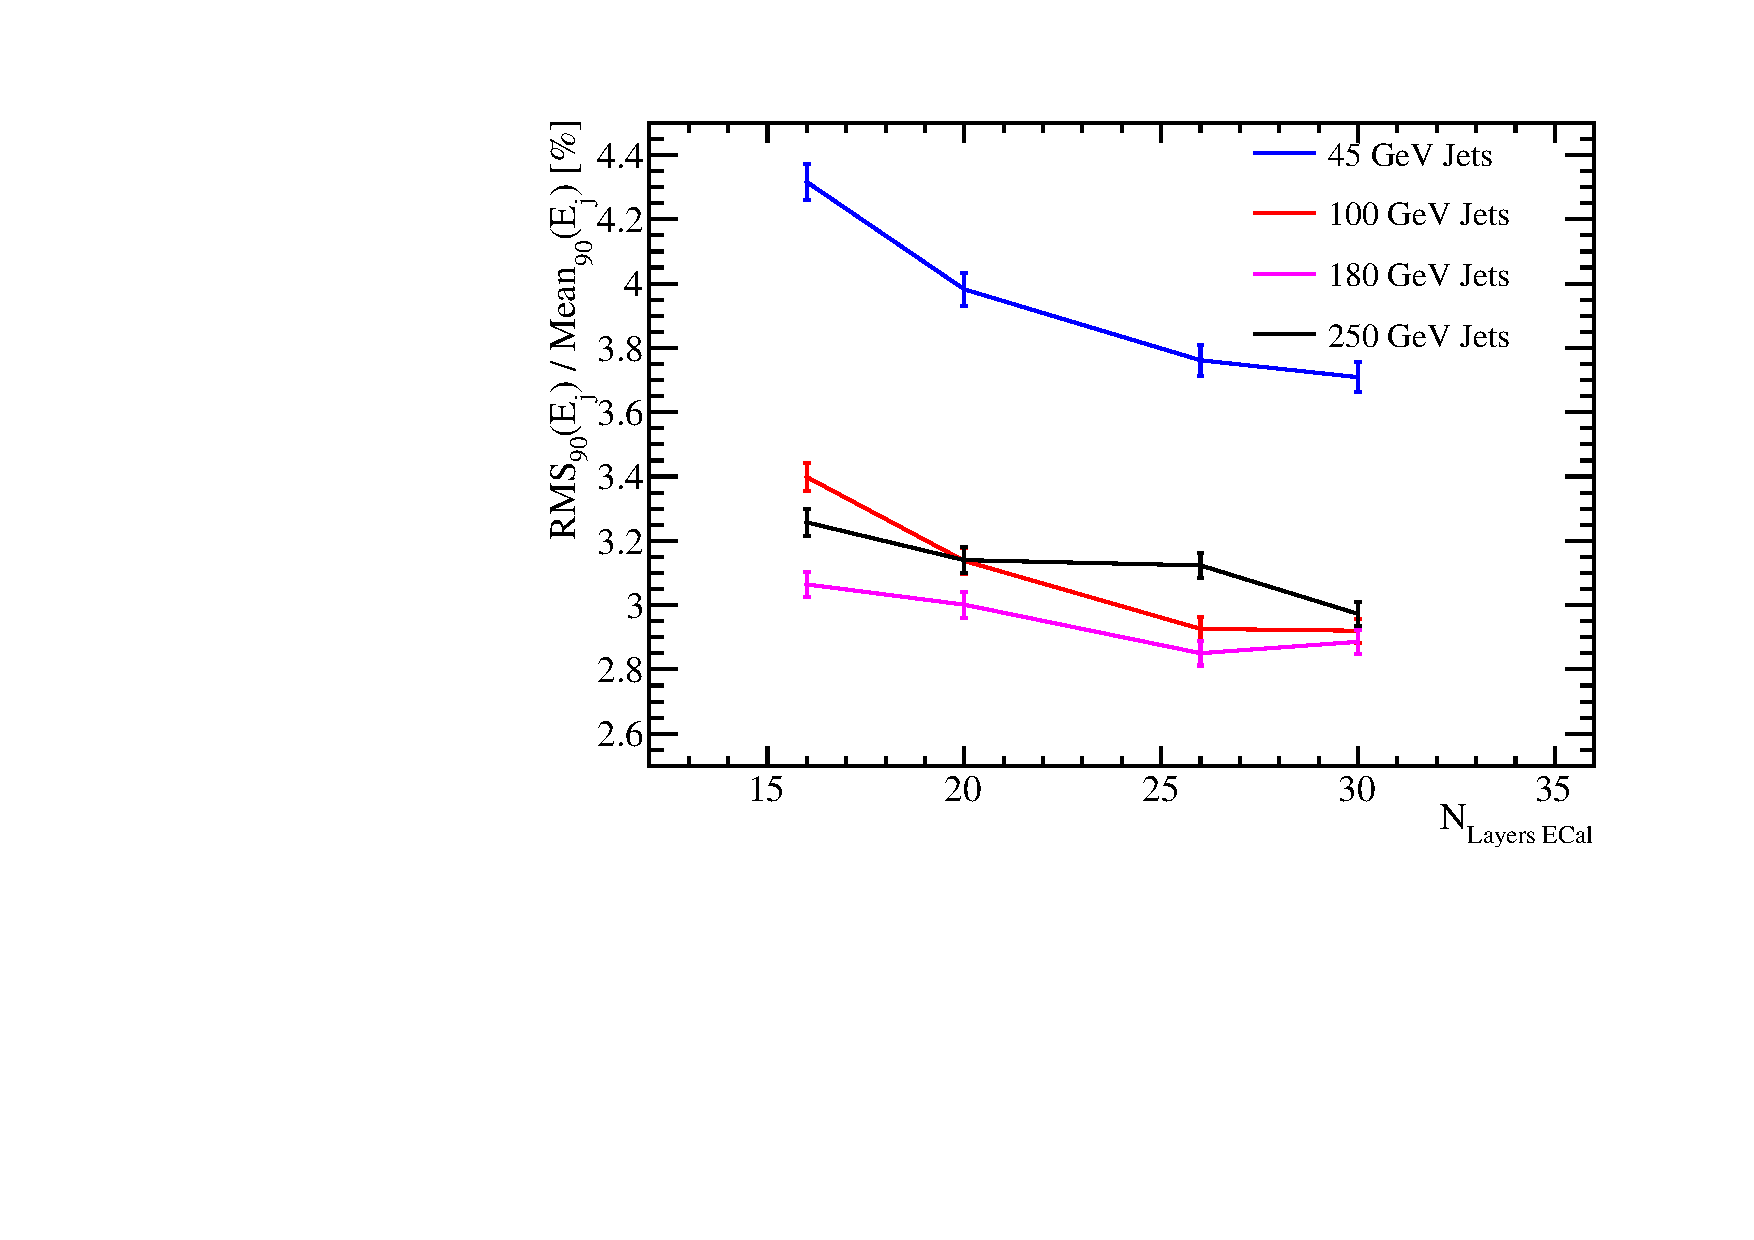
\includegraphics[width=0.5\textwidth]{OptimisationStudies/Plots/JetEnergyResolutions/JER_vs_SiliconECalNumberofLayers.pdf}}
\subfloat[]{\label{fig:ecalscnlayers}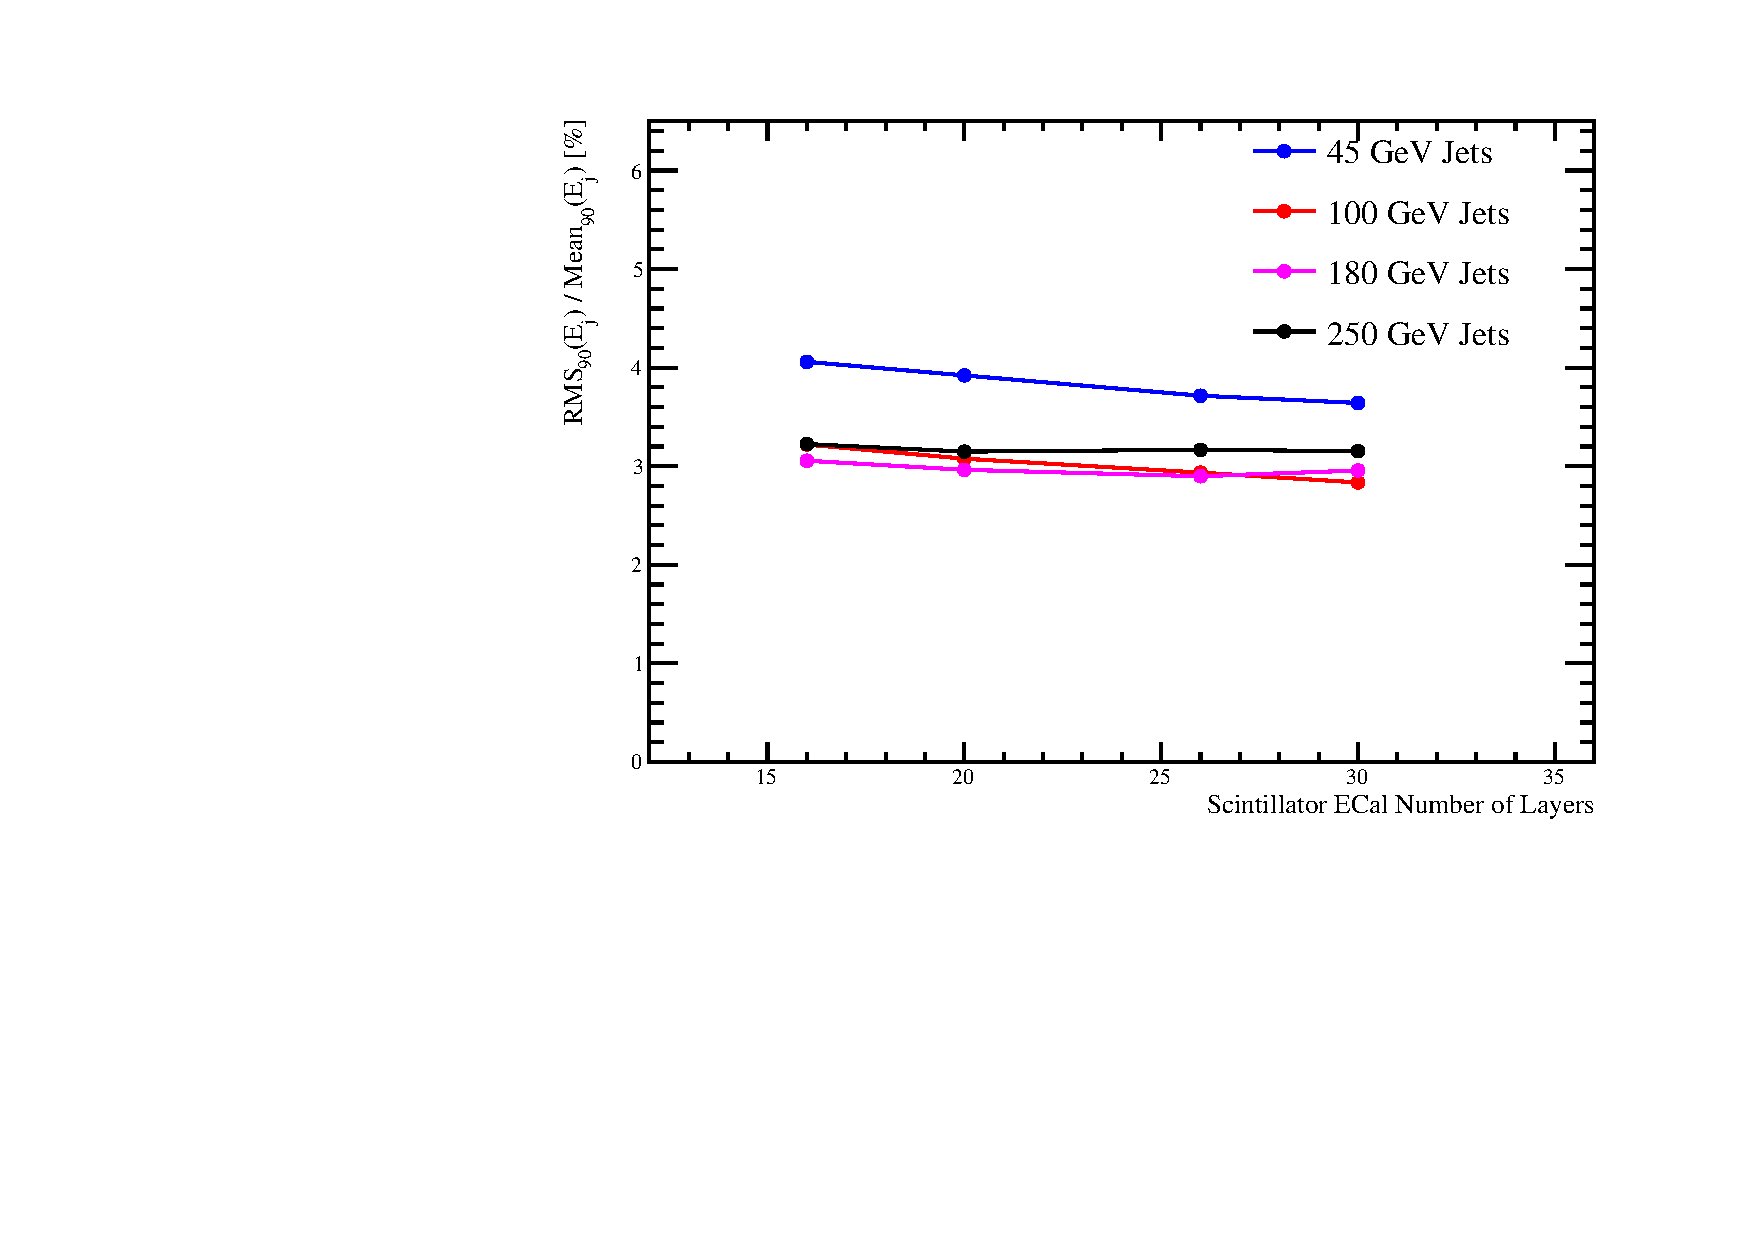
\includegraphics[width=0.5\textwidth]{OptimisationStudies/Plots/JetEnergyResolutions/JER_vs_ScintillatorECalNumberofLayers.pdf}} \hfill
\caption[The jet energy resolution as a function of number of layers in the ECal for various jet energies using the nominal ILD detector model with \protect\subref{fig:ecalsinlayers} the silicon and \protect\subref{fig:ecalscnlayers} the scintillator ECal option.]{The jet energy resolution as a function of number of layers in the ECal for various jet energies using the nominal ILD detector model with \protect\subref{fig:ecalsinlayers} the silicon and \protect\subref{fig:ecalscnlayers} the scintillator ECal option.}
\label{fig:ecalnlayers}
\end{figure}

% JER BD
% MAYBE REMOVE PHOTON CONFUSION
\begin{figure}
\centering
\subfloat[Silicon active material, 45 GeV Jets.]{\label{fig:ecalsinlayers45break}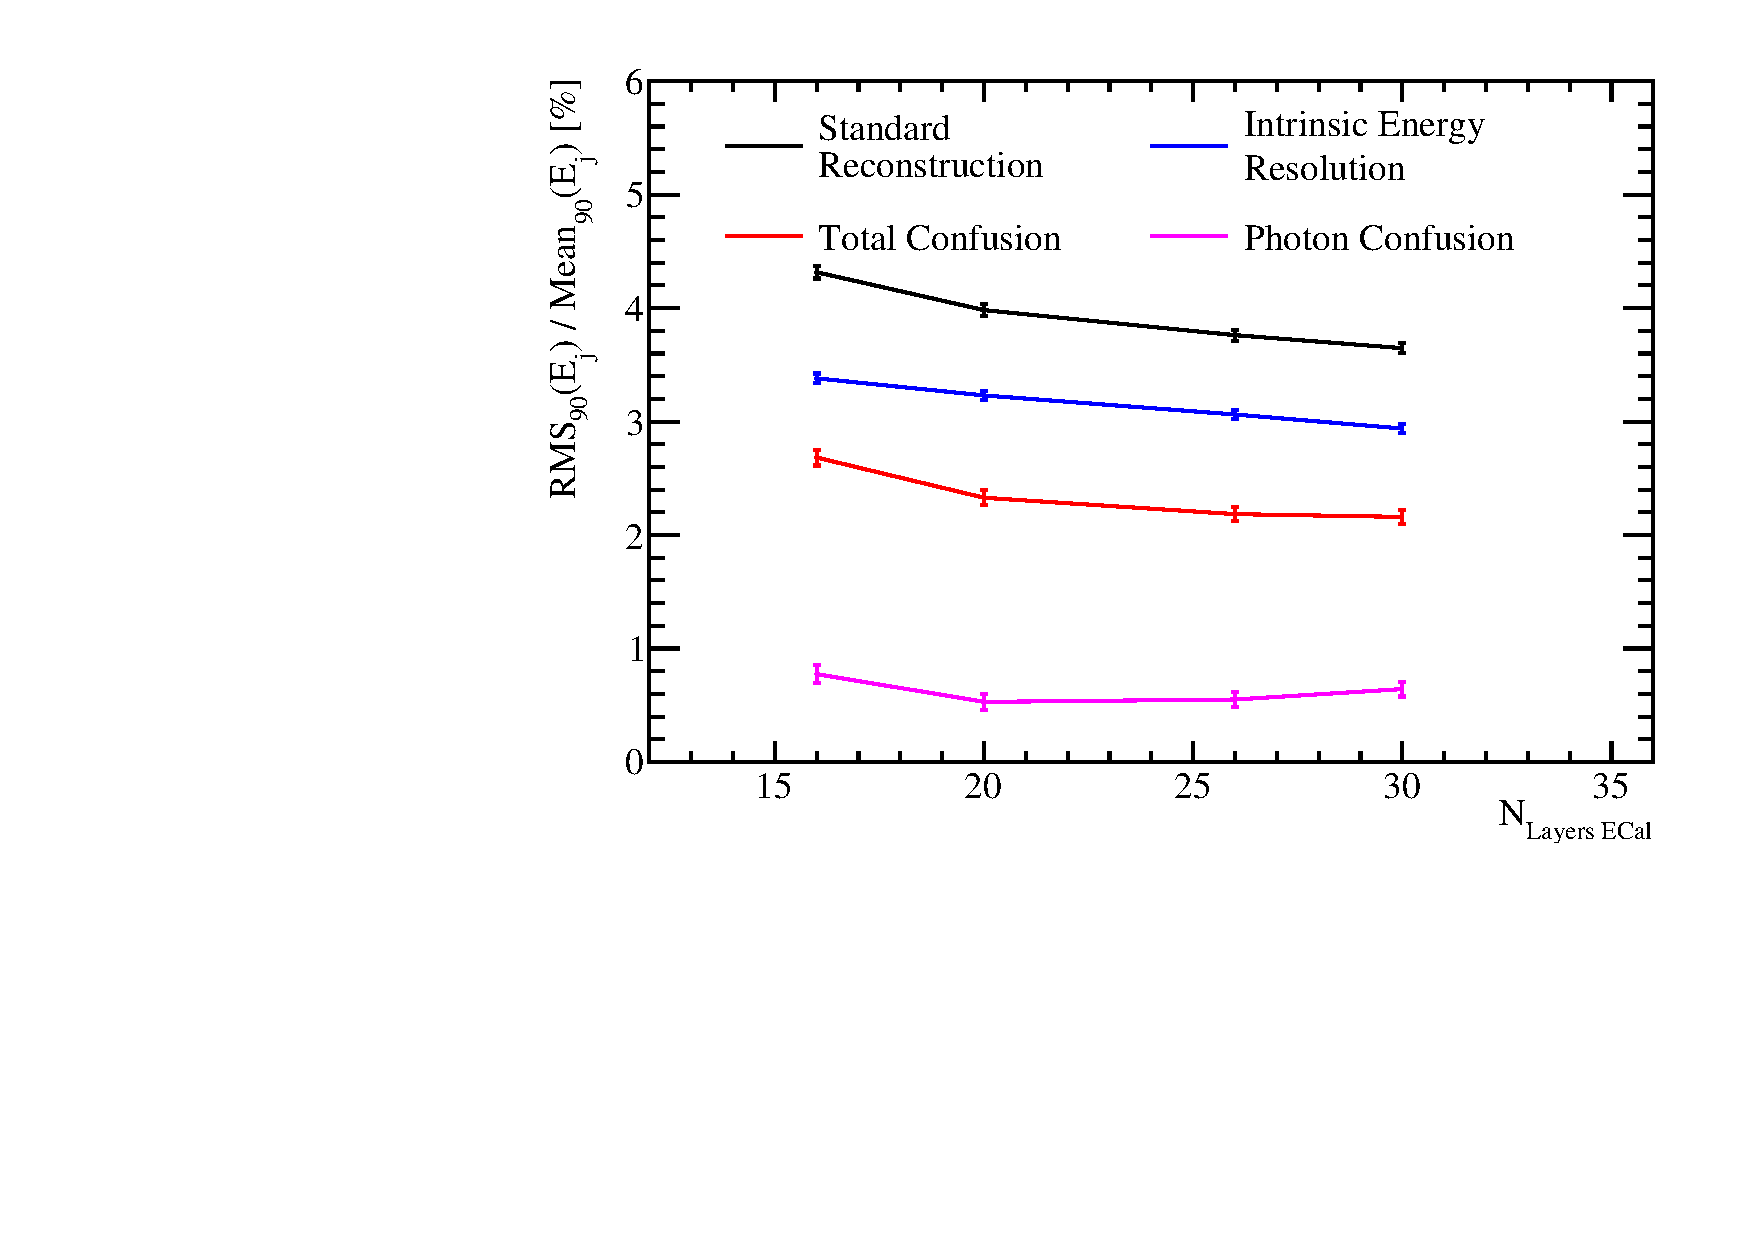
\includegraphics[width=0.5\textwidth]{OptimisationStudies/Plots/JetEnergyResolutions/JER_vs_SiliconECalNumberofLayers_91GeV_DiJet_Breakdown.pdf}}
\subfloat[Scintillator active material, 45 GeV Jets.]{\label{fig:ecalscnlayers45break}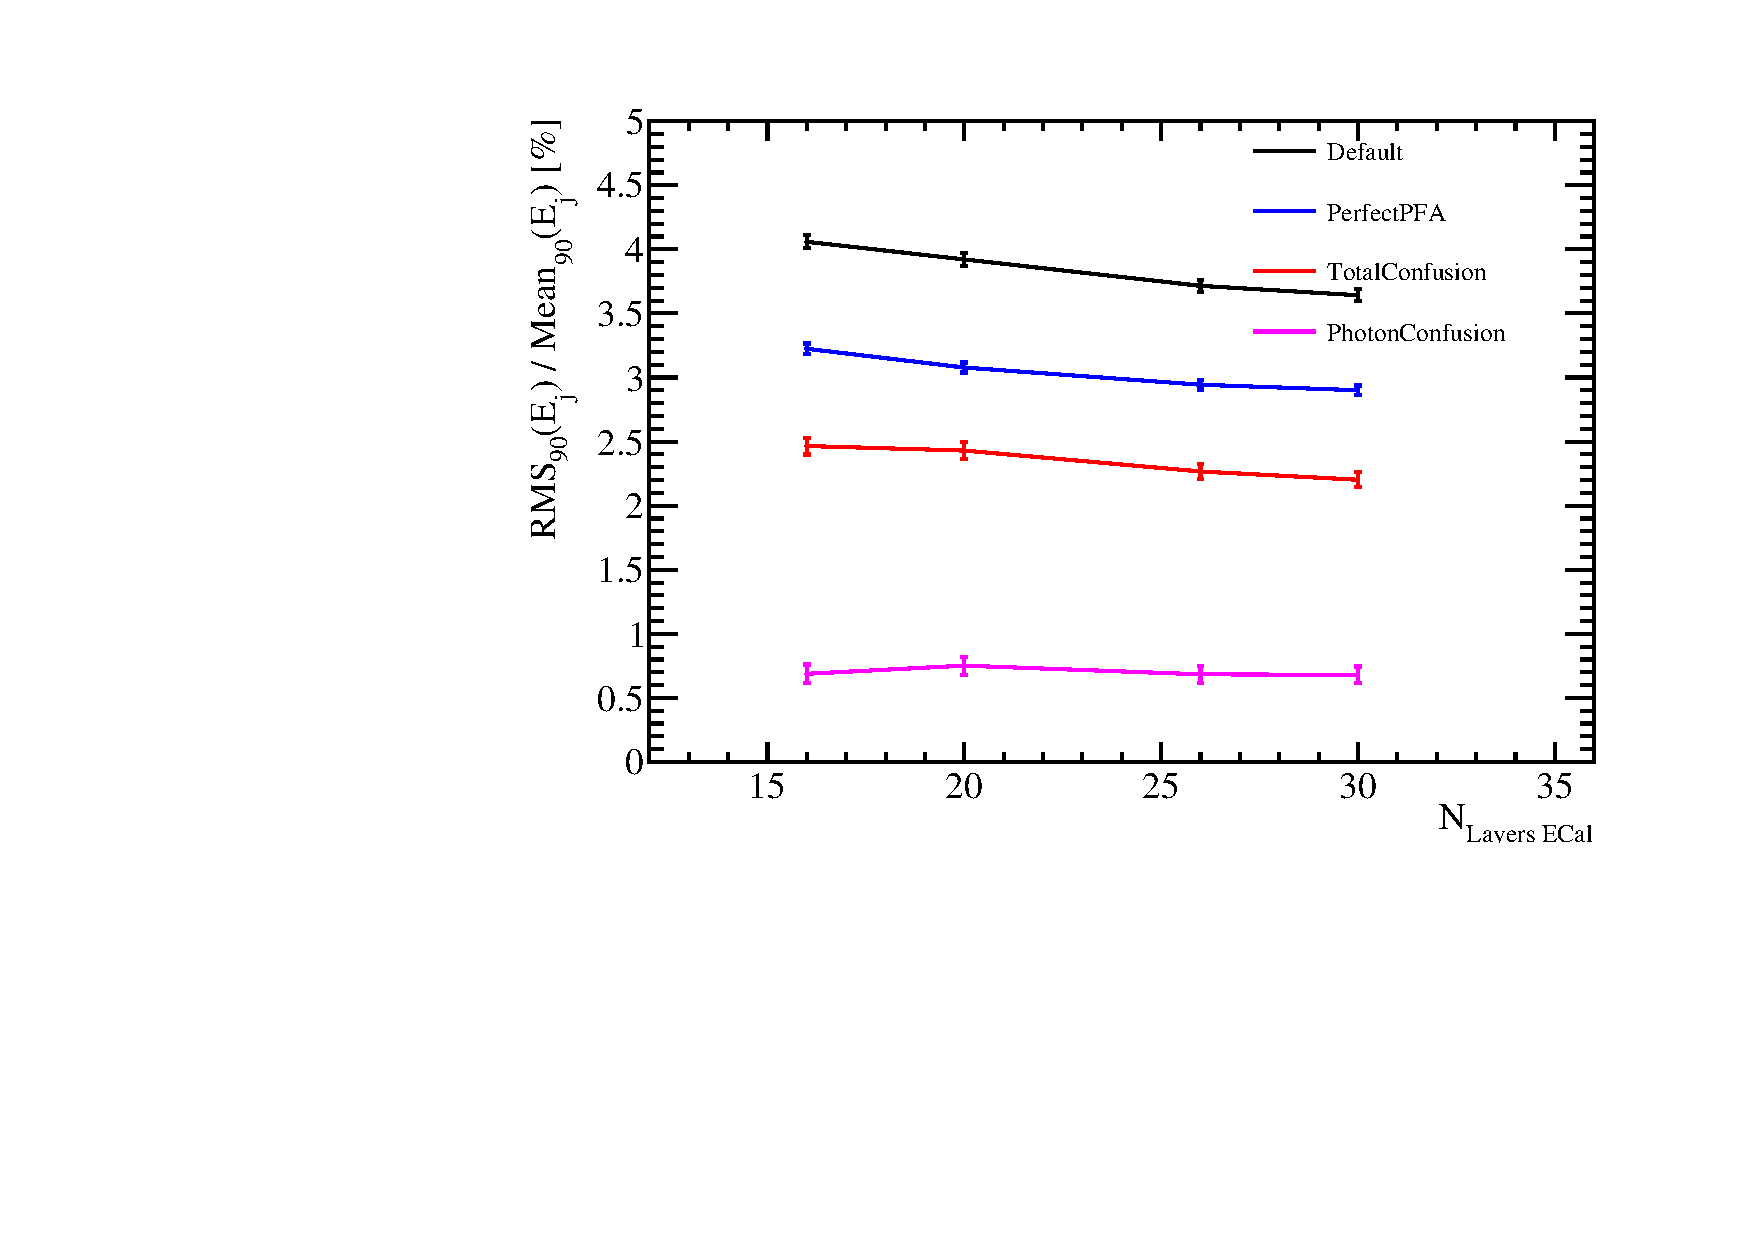
\includegraphics[width=0.5\textwidth]{OptimisationStudies/Plots/JetEnergyResolutions/JER_vs_ScintillatorECalNumberofLayers_91GeV_DiJet_Breakdown.pdf}} \hfill
\subfloat[Silicon active material, 250 GeV Jets.]{\label{fig:ecalsinlayers250break}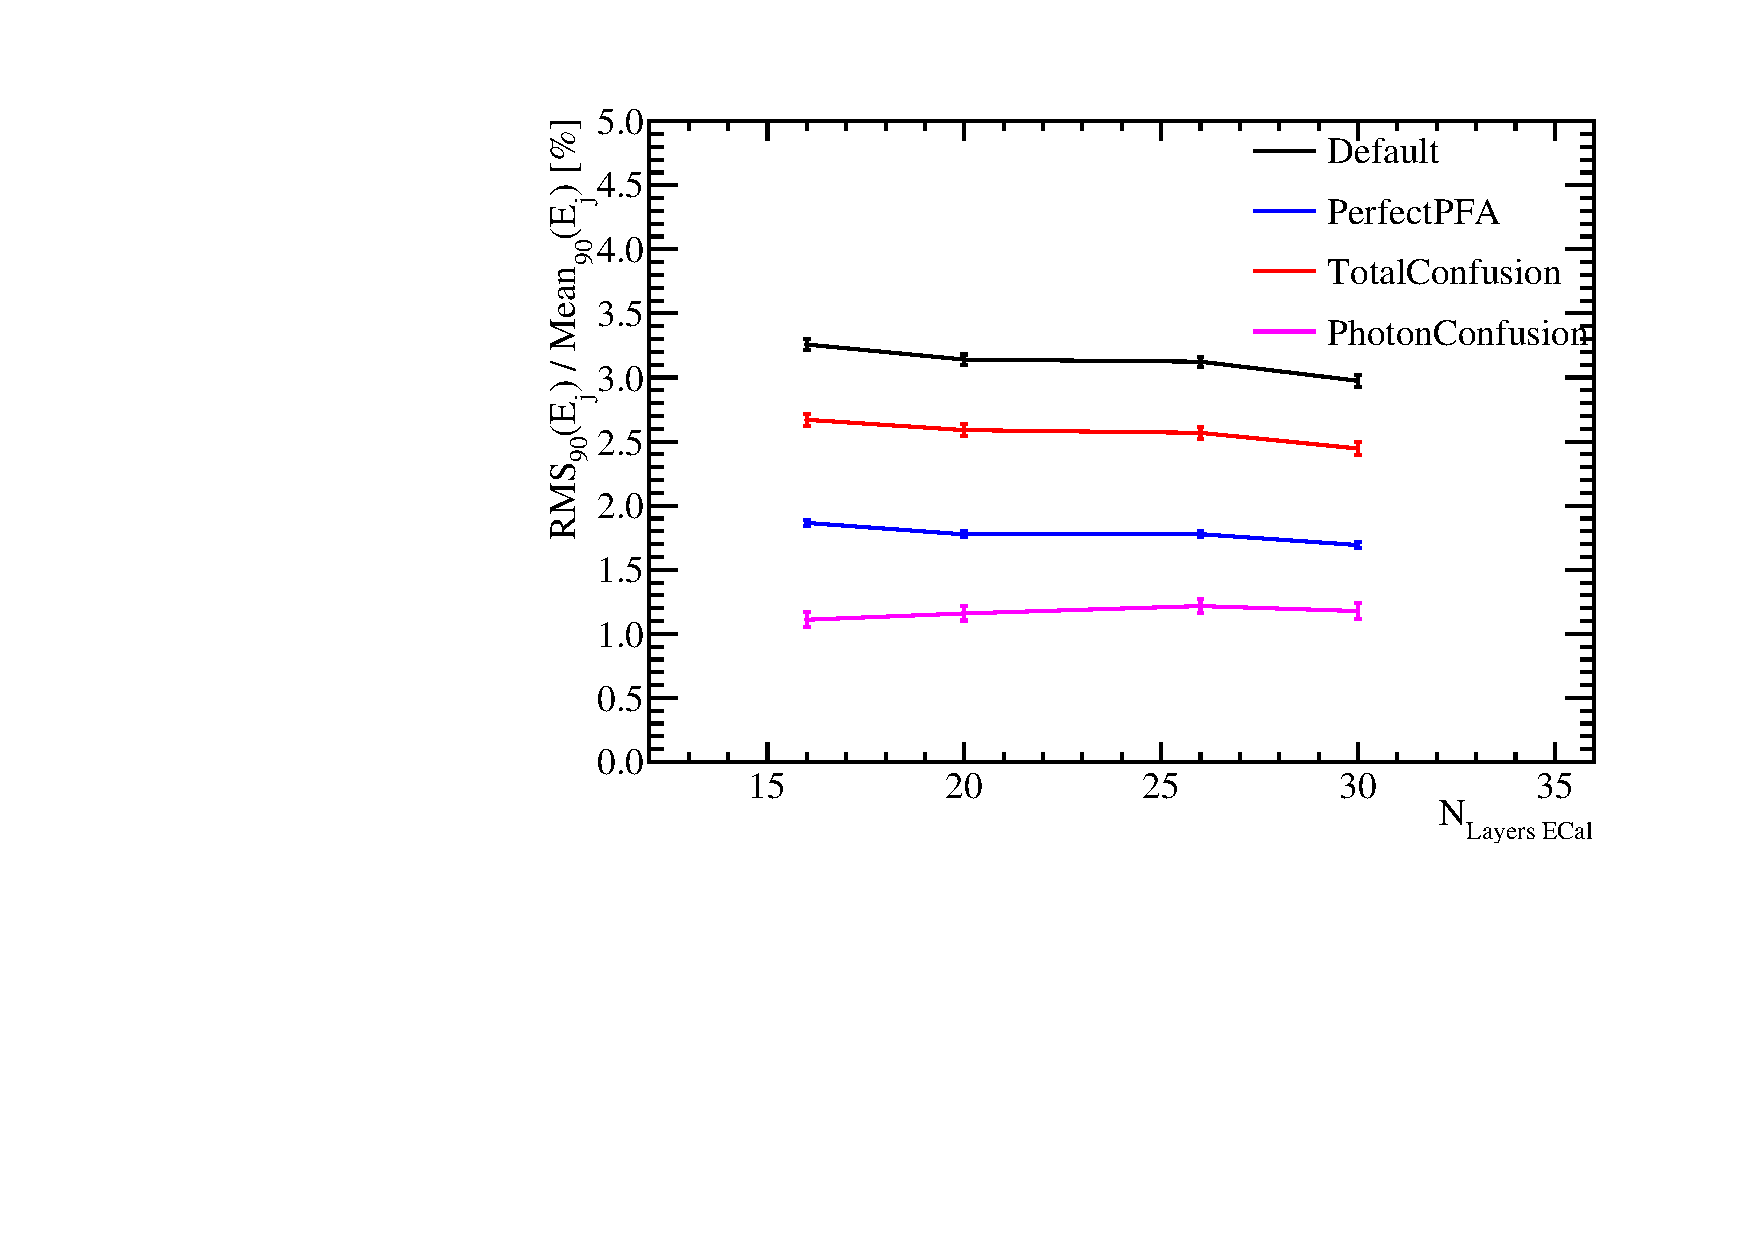
\includegraphics[width=0.5\textwidth]{OptimisationStudies/Plots/JetEnergyResolutions/JER_vs_SiliconECalNumberofLayers_500GeV_DiJet_Breakdown.pdf}}
\subfloat[Scintillator active material, 250 GeV Jets.]{\label{fig:ecalscnlayers250break}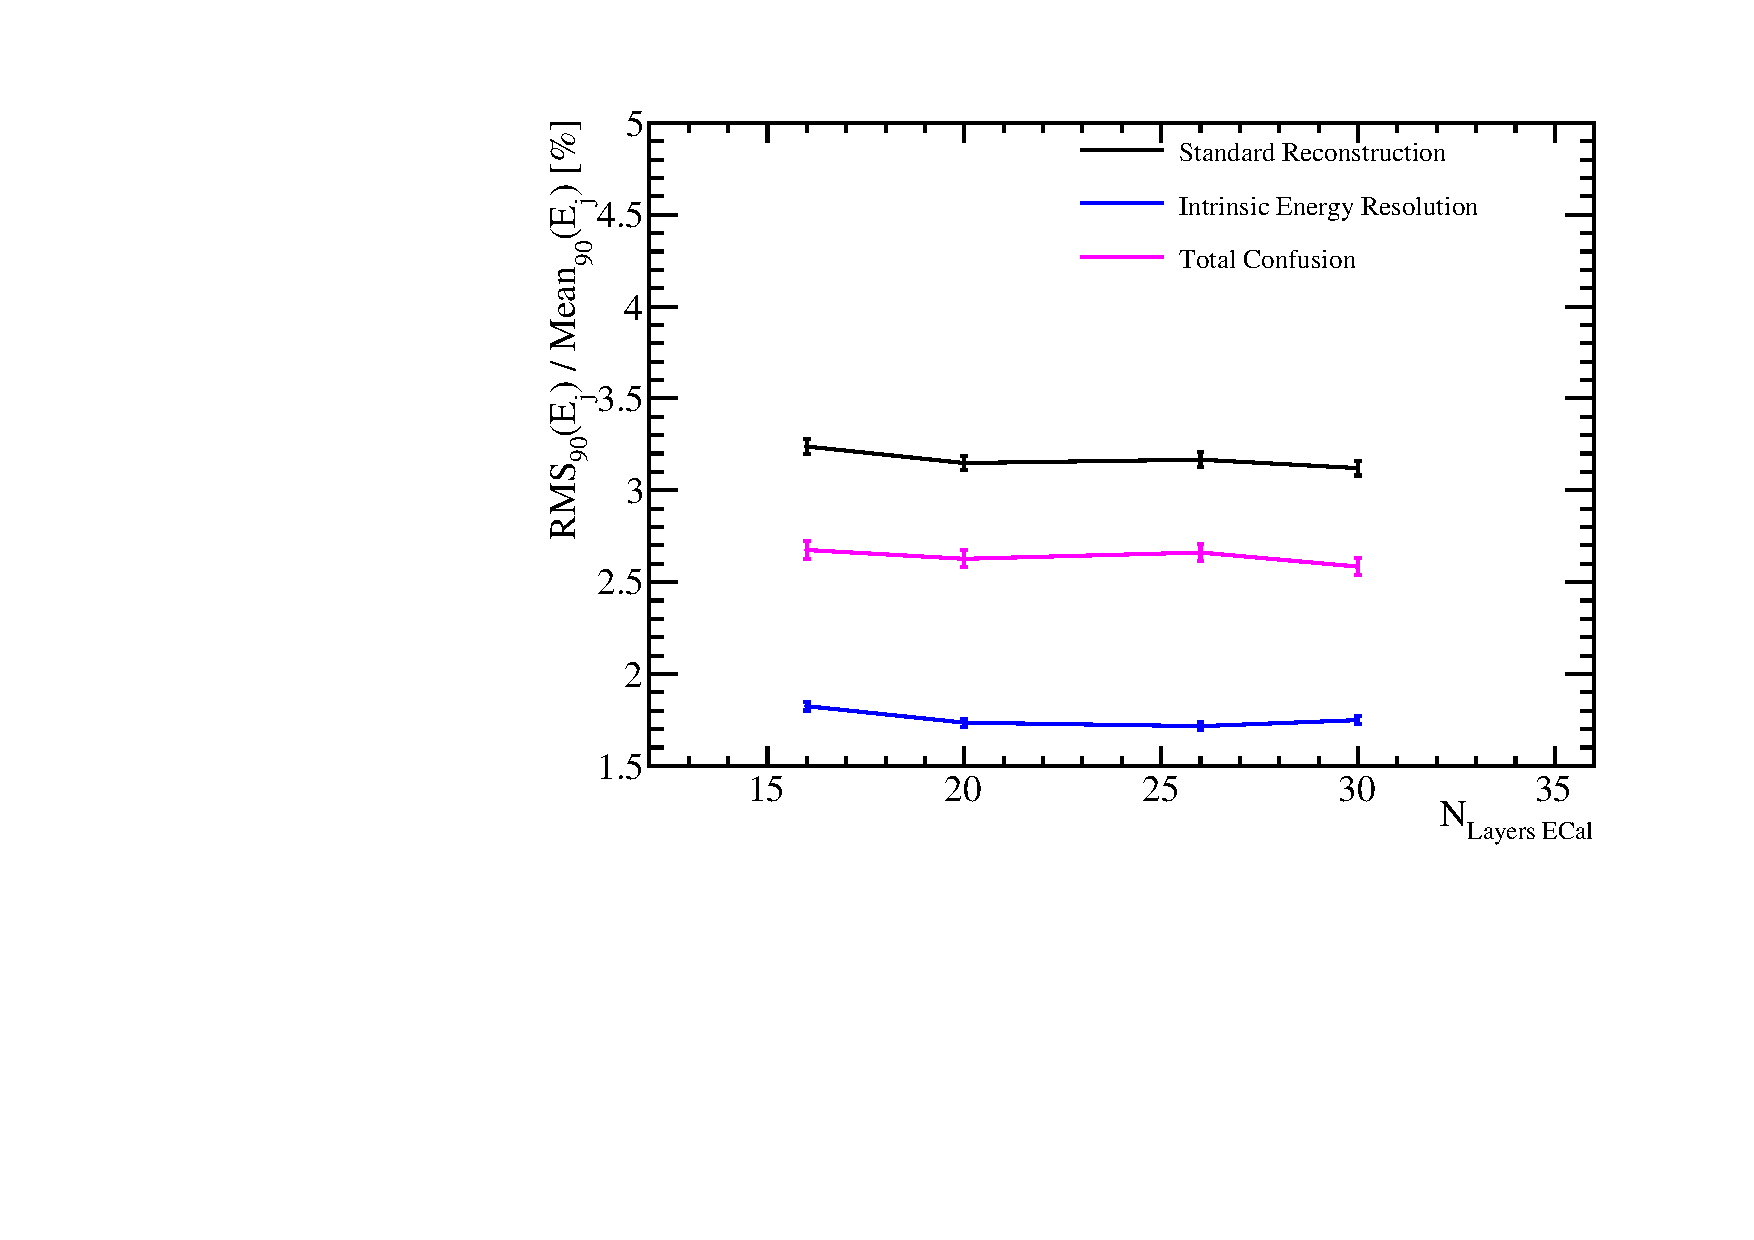
\includegraphics[width=0.5\textwidth]{OptimisationStudies/Plots/JetEnergyResolutions/JER_vs_ScintillatorECalNumberofLayers_500GeV_DiJet_Breakdown.pdf}}
\caption[The contributions to the jet energy resolution as a function of number of layers in the ECal using the nominal ILD detector model for \protect\subref{fig:ecalsinlayers45break} the silicon ECal option and 45 GeV jets, \protect\subref{fig:ecalscnlayers45break} the scintillator ECal option and 45 GeV jets, \protect\subref{fig:ecalsinlayers250break} the silicon ECal option and 250 GeV jets and \protect\subref{fig:ecalscnlayers250break} the scintillator ECal option and 250 GeV jets.  The black curve correspond to the standard reconstruction, the blue curve to the intrinsic energy resolution contribution to the jet energy resolution, the red curve to the confusion contribution to the jet energy resolution and the magenta curve to the confusion contribution to the jet energy resolution related solely to $\gamma$ reconstruction.]{The contributions to the jet energy resolution as a function of number of layers in the ECal using the nominal ILD detector model for \protect\subref{fig:ecalsinlayers45break} the silicon ECal option and 45 GeV jets, \protect\subref{fig:ecalscnlayers45break} the scintillator ECal option and 45 GeV jets, \protect\subref{fig:ecalsinlayers250break} the silicon ECal option and 250 GeV jets and \protect\subref{fig:ecalscnlayers250break} the scintillator ECal option and 250 GeV jets.  The black curve correspond to the standard reconstruction, the blue curve to the intrinsic energy resolution contribution to the jet energy resolution, the red curve to the confusion contribution to the jet energy resolution and the magenta curve to the confusion contribution to the jet energy resolution related solely to $\gamma$ reconstruction.}
\label{fig:ecalnlayersbreak}
\end{figure}

%========================================================================================

\subsection{ECal Active Material}
In sections \ref{sec:ecalcells} and \ref{sec:ecalnlayers} the performance of the ECal was reported for both the silicon and scintillator options and to a large extent the performance of the two options was the similar, but not identical:

\begin{itemize}
\item The intrinsic energy resolution of the silicon ECal option is better than that of a scintillator option for high energies, see figures \ref{fig:ecalsinominalres} and \ref{fig:ecalscnominalres}.  This is most likely due to the implementation of Birks' law \cite{BirksLaw} for scintillator active materials.  Birks' law states:
\begin{equation}
\frac{d\mathcal{L}}{dx} \propto \times \frac{dE/dx}{1+k_{B}dE/dx}
\end{equation}
where $\frac{d\mathcal{L}}{dx}$ is the light yield per unit path length, $dE/dx$ is the energy deposited per unit path length and $k_{B}$ is a material property constant.  For large energy deposits per unit length, such as those found in high energy $\gamma$ events, the light yield saturates causing a degradation in the energy resolution.  Based on a comparison with the silicon ECal option performance, this effect starts to degrade the energy resolution for the scintillator option around ~50 GeV.  However, the degradation in energy resolution up to 100 GeV is relatively small.
\item The "dead" region due to the presence of the MPPC in the simulation of the scintillator ECal option degrades performance of the detector for small transverse granularities, see figure \ref{fig:ecalcellsizegamma}.
\end{itemize}

In summary, the performance of the two options in terms of energy and jet energy resolution are similar meaning no clear option is preferred.  However, the silicon option is preferred when manufacture and implementation of the two models is compared.  While constructing silicon wafers to fit the $5 \times 5 \text{mm}^{2}$ square cell size of the ECal is achievable, this would be extremely challenging for scintillator tiles.  To resolve this in reality the scintillator ECal option would have to use $5 \times 45 \text{mm}^{2}$ scintillator strips that are arranged in alternating directions in each ECal layer.  By combining information from neighbouring layers it becomes possible to effectively achieve a $5 \times 5 \text{mm}^{2}$ square cell size.  This further challenges to the reconstruction means that the silicon option is the more preferred ECal model.  

%========================================================================================
%========================================================================================

\section{Hadronic Calorimeter Optimisation}
The HCal primarily measures energy deposits from hadronic showers.  The HCal in the default ILD detector model, summarised in table \ref{table:defaultildhcal}, and is approximately 6 nuclear interaction lengths ($\lambda_{I}$) deep.  The ECal contributes approximately one $\lambda_{I}$ giving a total of $\approx 7 \lambda_{I}$, which is sufficient to confine the bulk of jets up to 1 TeV events.  The longitudinal structure of this model consists of 48 readout layers each containing a 3 mm active layer of scintillator and a 20 mm absorber layer of iron.  

There are several readout approaches under consideration for the HCal including fully analogue, fully digital and semi-digital.  The analogue readout measures the energy within each HCal cell using a continuous spectrum of possible values, while the digital readout only produces a response if the energy deposited within a calorimeter cell is above a given threshold.  The semi-digital approach mirrors that of the digital approach, but has three responses each with a different energy threshold.  While the energy resolution for digital calorimeters is not as good as that of analogue calorimeters the advantage they have is that it is possible to construct smaller calorimeter cells using a digital readout.  In traditional calorimetry, a digital readout would only lead to a worsening energy resolution, however, in the particle flow paradigm pattern recognition is as important, if not more important, than energy resolution.  As the calorimeter cell size governs the confusion contribution to the jet energy resolution, it is envisaged that the use of a digital readout would involve a trade off where intrinsic energy resolution is sacrificed for a reduction in the pattern recognition confusion.  In the following studies only the analogue HCal is considered.

\begin{table}[h!]
\centering
\begin{tabular}{ l l}
\hline
Parameter & Default Value \\
\hline
Cell Size & $30 \times 30 \text{mm}^{2}$ square cells \\
Number of Layers & 48 readout layers \\
Active Material Choice & Scintillator \\
Active Material Thickness & 3 mm  \\
Absorber Material Choice & Steel \\
Absorber Material Thickness & 20 mm \\
\hline
\end{tabular}
\caption[The configuration of the HCal in the nominal ILD detector model.]{The configuration of the HCal in the nominal ILD detector model.}
\label{table:defaultildhcal}
\end{table}

% Nuclear interaction length iron 167.7mm
% Nuclear interaction length tungsten 99.46mm 
% Nuclear interaction length silicon 465.2mm 
% Nuclear interaction length polystyrene 770.7mm

The HCal performance for single hadrons and the overall jet energy resolution will depend on the details of the HCal design.  A number of options were simulated where the following parameters were varied:
\begin{itemize}
\item Cell size.  This is key to successful application of pattern recognition in the particle flow paradigm, but should not change the intrinsic energy resolution.   
\item Number of layers .  This governs the intrinsic energy resolution of a sampling calorimeter.
\item Depth of calorimeter.  This is important in determining the impact of leakage of energy out of the detector.  
\item Sampling fraction.  This is the ratio of the active medium thickness to the absorber medium thickness.  This controls how particle showers within the calorimeter are sampled.
\item Absorber material choice.  Two options have been considered: steel and tungsten.  This choice dictates the growth and propagation of hadronic showers and so plays a crucial role in calorimetry.  
\end{itemize}

%========================================================================================

% MOVE TO FIT ORDER OF BULLET POINTS
\subsection{HCal Absorber Material}
\label{sec:hcalabsorbermaterial}

The nominal choice of absorber material is steel, tungsten provides a feasible alternative material.  Although tungsten is more expensive than steel, it contains a larger number of nuclear interaction lengths per unit length.  Therefore, using tungsten as opposed to steel as the absorber material would reduce the size of the HCal, while retaining the same number of nuclear interaction lengths.  Reducing the depth of the calorimeter would decrease the size of the solenoid required, which would offset some of the additional cost if tungsten were used as the absorber material. 

\begin{table}[h!]
\centering
\begin{tabular}{ l l l }
\hline
Parameter & Steel HCal Option & Tungsten HCal Option \\
\hline
Cell Size & $30 \times 30 \text{mm}^{2}$ square cells & $30 \times 30 \text{mm}^{2}$ square cells\\
Number of Layers & 48 readout layers & 48 readout layers\\
Absorber Material Thickness [mm] & 20.0 & 12.0 \\
Active Material Choice & Scintillator & Scintillator \\
Active Material Thickness [mm] & 3.0 & 1.8 \\
\hline
\end{tabular}
\caption[The configuration of the stainless steel and tungsten HCal options.]{The configuration of the stainless steel and tungsten HCal options.}
\label{table:hcalabsmaterial}
\end{table}

The configuration for the stainless steel and tungsten HCal options that were used in the full ILD simulation can be found in table \ref{table:hcalabsmaterial}.  To isolate the effects of changing the absorber material, the total depth, in nuclear interaction lengths, was kept constant when comparing these two options.  Furthermore, the sampling fraction, the ratio of active to absorber layer thickness, was also held constants.  The interaction of hadrons with the absorber material within the detector is simulated by GEANT4.  A number of different physics lists exist within GEANT4 for the modelling of hadronic showers.  The default model for high energy physics calorimetry is the QGSP\_BERT physics list, which uses the quark-gluon string model \cite{Folger:2003sb} with the precompound model of nuclear evaporation \cite{geantStringModel} (QGSP) for high energy interactions and the Bertini (BERT) cascade model \cite{Guthrie:1968ue} for intermediate energy interactions.  For this study both the QGSP\_BERT and the QGSP\_BERT\_HP physics lists were used.  The QGSP\_BERT\_HP list uses the high precision neutron package (NeutronHP) to deal with the transportation of neutrons from below 20 MeV to thermal energies.  This added detail was thought to be necessary for a study involving tungsten due to the expected increase in shower development.    

% Timing

One of the dominant process governing the energy deposition of hadronic showers in calorimeters is spallation \cite{Wigmans:2000vf}.  Spallation begins with the collision of a high energy incident particle with an atomic nuclei from the calorimeter absorbing material.  This collision creates an internuclear cascade where a shower of high energy hadronic particles, e.g. protons, neutrons and pions, are produced within the nucleus.  If these energies are large enough some of these particles may escape the nucleus and form secondary particles in the hadronic shower.  After this initial collision the nuclei of the absorbing material are left in an excited state.  Assuming the excited nuclei are sufficiently stable that they will not undergo fission, they will return to a stable state by ejecting energy in the form of particles in a process called evaporation.  Evaporation of neutrons, which is the dominant form of evaporation, significantly delays the growth of hadronic showers as some of these neutrons undergo neutron capture \cite{Adloff:2014rya}.  Neutron capture involves an absorber nuclei capturing a neutron and then emitting a $\gamma$ as it returns to a stable state.  Therefore, the time it take for the neutron capture mechanism to proceed is limited by the lifetime of the unstable nuclei.  This makes neutron capture one of the slowest mechanisms by which hadronic showers can propagate.  As absorber materials with a large atomic number, Z, have a larger number of neutrons, it is expected that there will be an increase in the number of evaporation neutrons within hadronic showers developing in such materials.  In turn this will lead to more neutron capture processes and a longer development time for the hadronic showers.  This is what is observed when considering the shower development times using the tungsten (Z=74) and steel (iron, Z=26) HCal options as seen in figure \ref{fig:hcalabsmaterialtiming}. 

% Maybe worth adding to timing chapter
%\begin{figure}
%\centering
%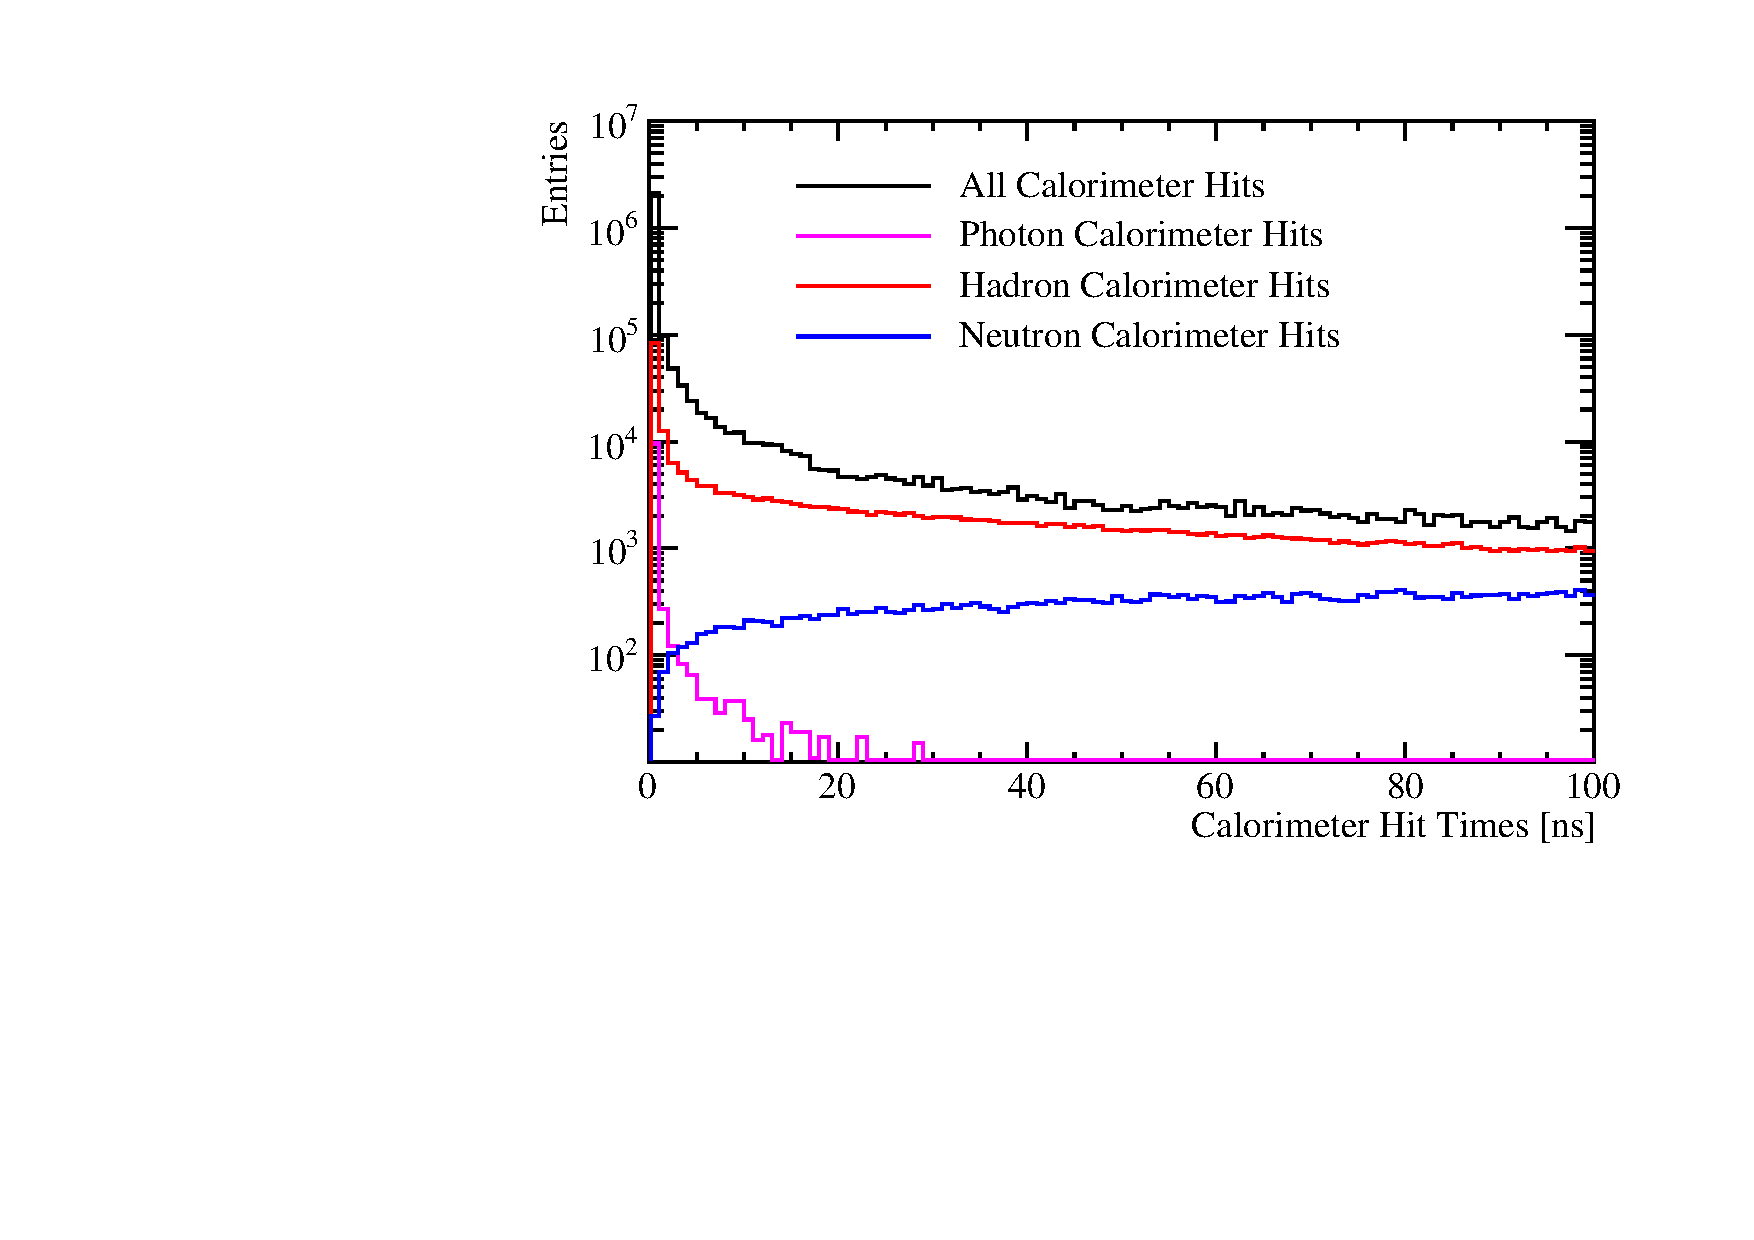
\includegraphics[width=0.5\textwidth]{OptimisationStudies/Plots/Description/CalorimeterHitTimes_91GeV_Z_uds_Steel.pdf}
%\caption[The distribution of the time of the calorimeter hits, corrected for time of flight to the impact point, for 91 GeV Z$\rightarrow$uds di-jet events.]{The distribution of the time of the calorimeter hits, corrected for time of flight to the impact point, for 91 GeV Z$\rightarrow$uds di-jet events.}
%\label{fig:calohittiming}
%\end{figure} 

\begin{figure}
\centering
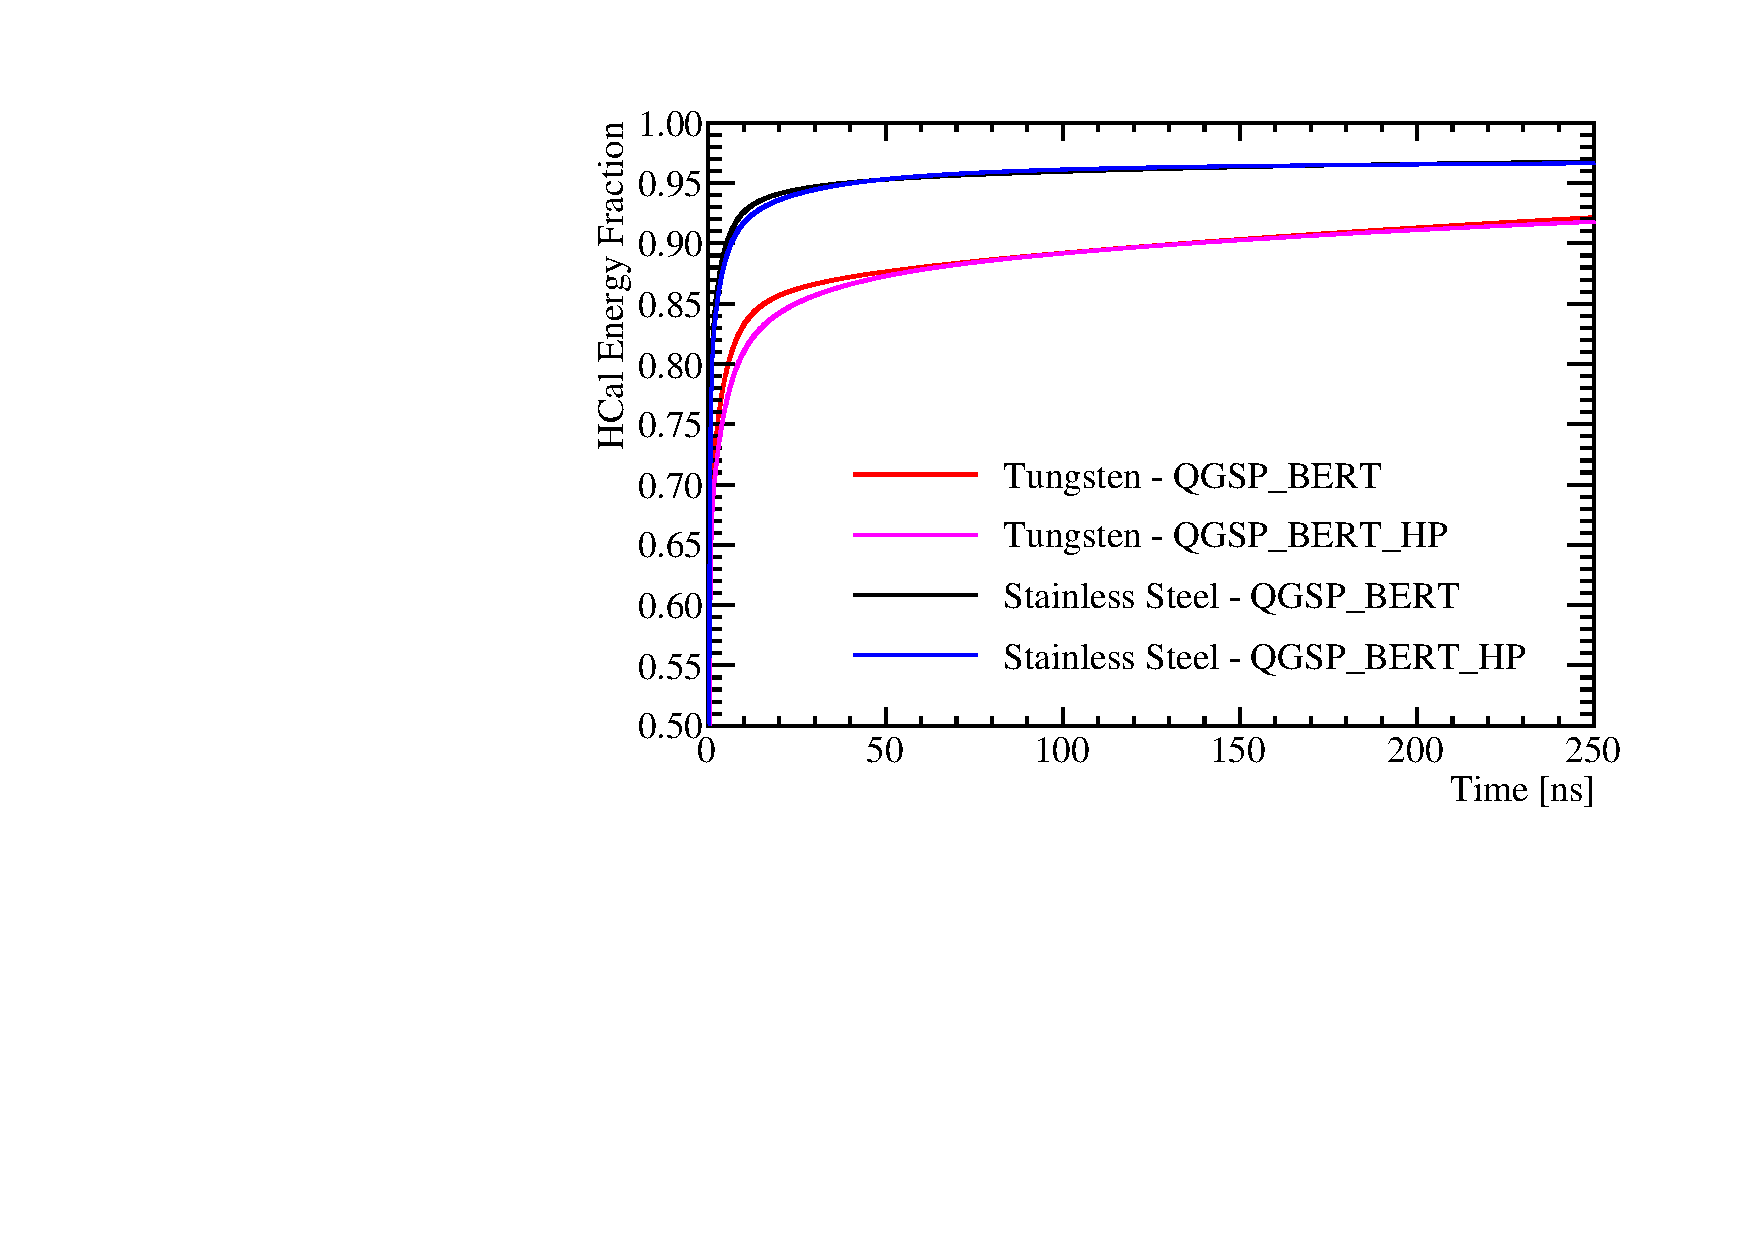
\includegraphics[width=0.5\textwidth]{OptimisationStudies/Plots/Description/HCalAbsorberMaterialTimings.pdf}
\caption[The fraction of the total calorimetric energy deposited in the HCal as a function of time for 25 GeV $\text{K}^{0}_{L}$ events using the steel and tungsten HCal options.  Results are shown for both the QGSP\_BERT and QGSP\_BERT\_HP physics lists.  The calorimeter hit times have been corrected for straight line time of flight to the impact point.]{The fraction of the total calorimetric energy deposited in the HCal as a function of time for 25 GeV $\text{K}^{0}_{L}$ events using the steel and tungsten HCal options.  Results are shown for both the QGSP\_BERT and QGSP\_BERT\_HP physics lists.  The calorimeter hit times have been corrected for straight line time of flight to the impact point.}
\label{fig:hcalabsmaterialtiming}
\end{figure} 

%SP

\begin{table}[h!]
\centering
\begin{tabular}{ l l l }
\hline
HCal Option & Energy Resolution [\%] \\
\hline
Stainless Steel, QGSP\_BERT & $8.8\pm0.2$ \\
Stainless Steel, QGSP\_BERT\_HP & $9.0\pm0.3$ \\
Tungsten, QGSP\_BERT & $9.1\pm0.2$ \\
Tungsten, QGSP\_BERT\_HP & $9.0\pm0.2$ \\
\hline
\end{tabular}
\caption[The energy resolution using the nominal ILD detector with various HCal options determined using 50 GeV $\text{K}^{0}_{L}$ events.]{The energy resolution using the nominal ILD detector with various HCal options determined using 50 GeV $\text{K}^{0}_{L}$ events.}
\label{table:erhcalabsmaterial}
\end{table}

The energy resolution for 50 GeV $\text{K}^{0}_{L}$ events using the nominal ILD detector model with a stainless steel and tungsten HCal absorber material can be found in table \ref{table:erhcalabsmaterial}.  No significant differences were seen in the energy resolution when changing the absorber material.  Furthermore, the addition of the high precision neutron package did not alter the detector performance significantly.    

%JER

\begin{table}[h!]
\centering
\begin{tabular}{ l l l l l }
\hline
HCal Option & Jet Energy & & & \\
 & Resolution & & & \\
 & [\%] & & & \\
 & 45 GeV & 100 GeV & 180 GeV & 250 GeV \\
\hline
Stainless Steel, QGSP\_BERT & $3.65 \pm 0.05$ &$2.88 \pm 0.04$ &$2.85 \pm 0.04$ &$2.97 \pm 0.05$ \\
Stainless Steel, QGSP\_BERT\_HP & $3.67 \pm 0.05$ &$2.92 \pm 0.04$ &$2.86 \pm 0.04$ &$3.03 \pm 0.04$ \\
Tungsten, QGSP\_BERT & $3.67 \pm 0.05$ &$3.12 \pm 0.04$ &$3.36 \pm 0.04$ &$3.76 \pm 0.05$ \\
Tungsten, QGSP\_BERT\_HP & $3.69 \pm 0.05$ &$3.03 \pm 0.04$ &$3.38 \pm 0.04$ &$3.80 \pm 0.05$ \\
\hline
\end{tabular}
\caption[The jet energy resolution using the nominal ILD detector with various HCal options for various jet energies.]{The jet energy resolution using the nominal ILD detector with various HCal options for various jet energies.}
\label{table:jerhcalabsmaterial}
\end{table}

The jet energy resolutions for various jet energies are shown in table \ref{table:jerhcalabsmaterial} for the various HCal options considered.  These results indicate that steel outperforms tungsten as an absorber material for high energy jets, while at low jet energies the performance is similar.  This indicates that the intrinsic energy resolution of the detector, which is the dominant contribution to the jet energy resolution at low jet energies, is similar for the steel and tungsten options, which is in agreement with the single $\text{K}^{0}_{L}$ energy resolution study.  At high jet energies the performance of the two models diverges, with the steel option giving the better performance.  The performance at high energies will be controlled by the confusion contribution to the jet energy resolution, which are shown for 45 and 250 GeV jets in table \ref{table:jerbdhcalabsmaterial}.  The confusion contribution is also larger for the tungsten option at low jet energies, however, as the intrinsic energy resolution of the detector dominates at these energies the effect of confusion is less prominent.  The change in confusion will be due to the PandoraPFA algorithms being tuned for HCal cell dimensions for the steel HCal option, while the cells for the tungsten option are thinner by a factor of approximately $\frac{\lambda_{I}^{Steel}}{\lambda_{I}^{Tungsten}} \approx 1.7$, where $\lambda_{I}^{x}$ is the distance of one radiation length in material $x$.  It is unfeasible to tune all of the PandoraPFA algorithms to each detector geometry, however, the breakdowns of the jet energy resolution indicate that even if it were possible to obtain the same confusion contributions to the jet energy resolution the intrinsic energy resolution of the tungsten option is marginally worse than that of steel.  

The energy resolution is marginally worse for the tungsten option at high energies in comparison to the steel option as... TRUNCATION MAYBE NEEDS CHANGING 

Therefore, tungsten offers no advantage to steel based on jet energy resolution.  

%%%While maybe make pandora more effective, not needed as tungsten ER worse marginally at high energies so only ever worse.

The use of the QGSP\_BERT\_HP physics list, as opposed to QGSP\_BERT, made a minimal impact on these results.

%JER BD

\begin{table}[h!]
\centering
\begin{tabular}{ l l l l l }
\hline
HCal Option & Jet Energy & & & \\
 & Resolution & & & \\
 & [\%] & & & \\
 & 45 GeV & & 250 GeV & \\
 & Intrinsic & Confusion & Intrinsic & Confusion \\
\hline
Stainless Steel, QGSP\_BERT & $2.93 \pm 0.04$ & $2.16 \pm 0.06$ & $1.69 \pm 0.02$ &$2.45 \pm 0.05$ \\
Stainless Steel, QGSP\_BERT\_HP & $2.98 \pm 0.04$ &$2.15 \pm 0.06$ &$1.65 \pm 0.02$ &$2.53 \pm 0.04$ \\
Tungsten, QGSP\_BERT & $2.94 \pm 0.04$ &$2.20 \pm 0.06$ &$1.80 \pm 0.02$ &$3.30 \pm 0.05$ \\
Tungsten, QGSP\_BERT\_HP & $2.89 \pm 0.04$ &$2.29 \pm 0.64$ &$1.75 \pm 0.02$ &$3.37 \pm 0.05$ \\
\hline
\end{tabular}
\caption[The contributions to the jet energy resolution using the nominal ILD detector with various HCal options for 45 and 250 GeV jet energies.]{The contributions to the jet energy resolution using the nominal ILD detector with various HCal options for 45 and 250 GeV jet energies.}
\label{table:jerbdhcalabsmaterial}
\end{table}

In conclusion, the steel option HCal outperforms the tungsten option in terms of intrinsic energy resolution and pattern recognition confusion making it the more preferred option of the two.

%========================================================================================

\subsection{HCal Cell Size}
\label{sec:hcalcells}
For this study a number of different detector models were considered where the cell size in the HCal had been varied about the nominal value of $30 \times 30 \text{mm}^{2}$ square cells.  The granularities considered were $10 \times 10 \text{mm}^{2}$, $20 \times 20 \text{mm}^{2}$, $30 \times 30 \text{mm}^{2}$, $40 \times 40 \text{mm}^{2}$, $50 \times 50 \text{mm}^{2}$ and $100 \times 100 \text{mm}^{2}$ square cells.  The jet energy resolution as a function of cell size in the HCal is shown in figure \ref{fig:hcalcellsize}.

\begin{figure}
\centering
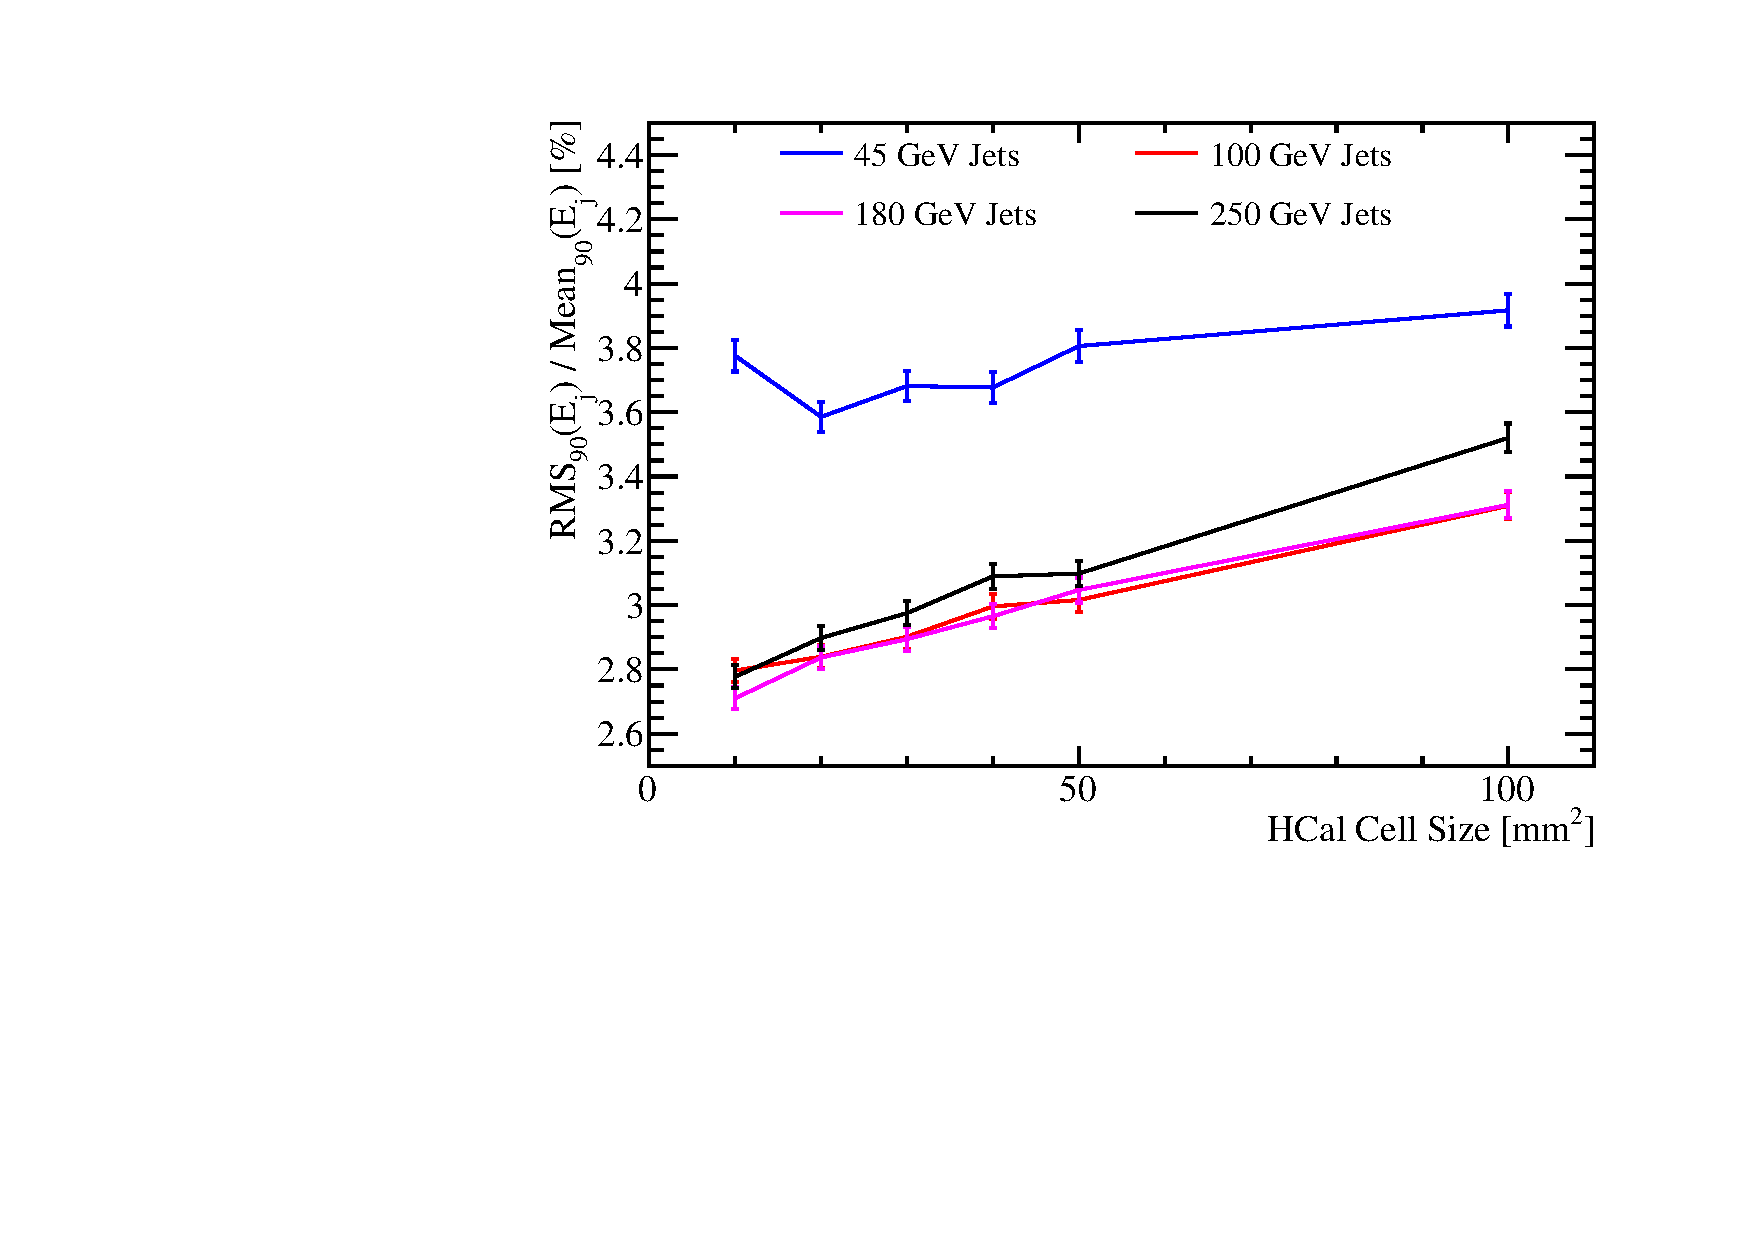
\includegraphics[width=0.5\textwidth]{OptimisationStudies/Plots/JetEnergyResolutions/JER_vs_HCalCellSize.pdf}
\caption[Jet energy resolution as a function of HCal cell size.]{Jet energy resolution as a function of HCal cell size.}
\label{fig:hcalcellsize}
\end{figure}

As with the case for the ECal, the jet energy resolution was found to improve with decreasing cell size as smaller cell size lead to better separation of energy deposits from neutral and charged particle showers.

\begin{figure}
\centering
\subfloat[45 GeV Jets.]{\label{fig:hcalcellsize45break}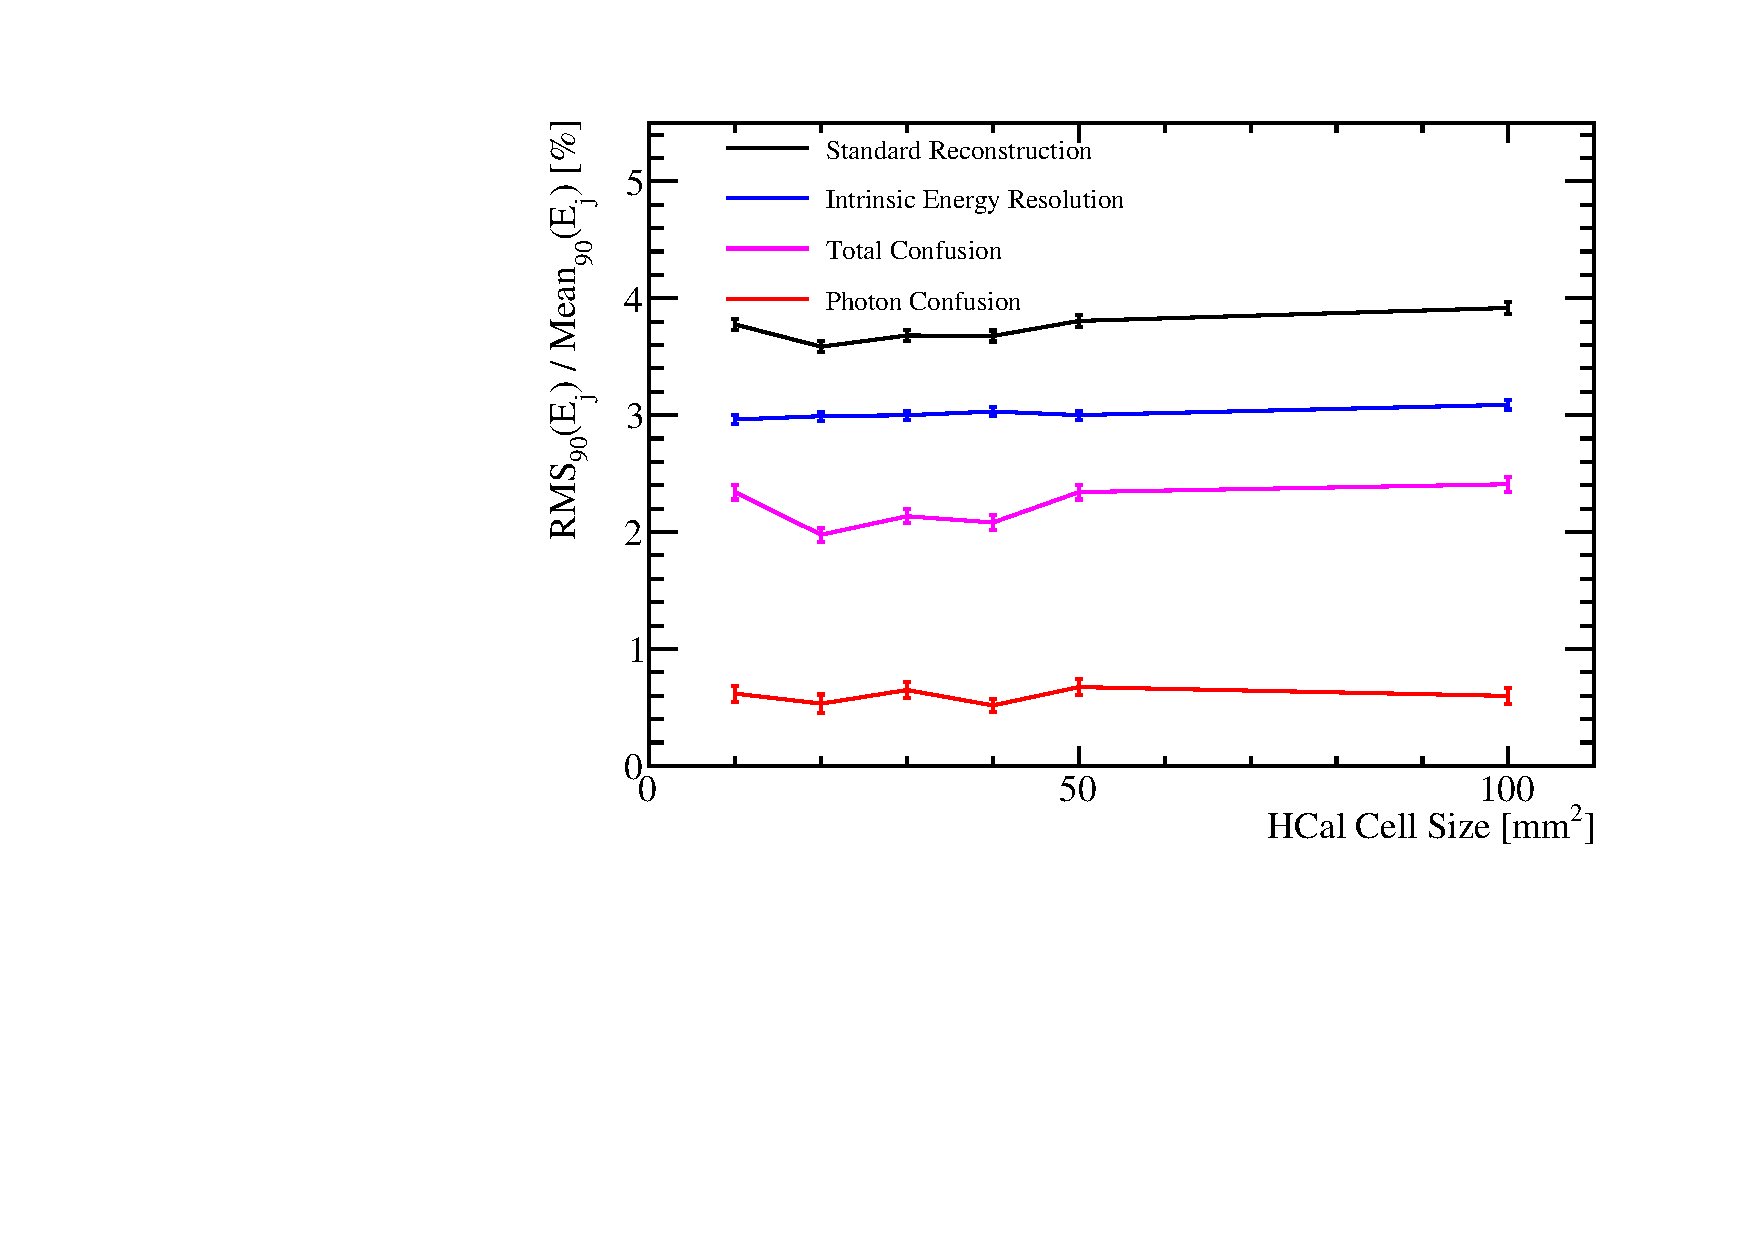
\includegraphics[width=0.5\textwidth]{OptimisationStudies/Plots/JetEnergyResolutions/JER_vs_HCalCellSize_91GeV_DiJet_Breakdown.pdf}}
\subfloat[250 GeV Jets.]{\label{fig:hcalcellsize250break}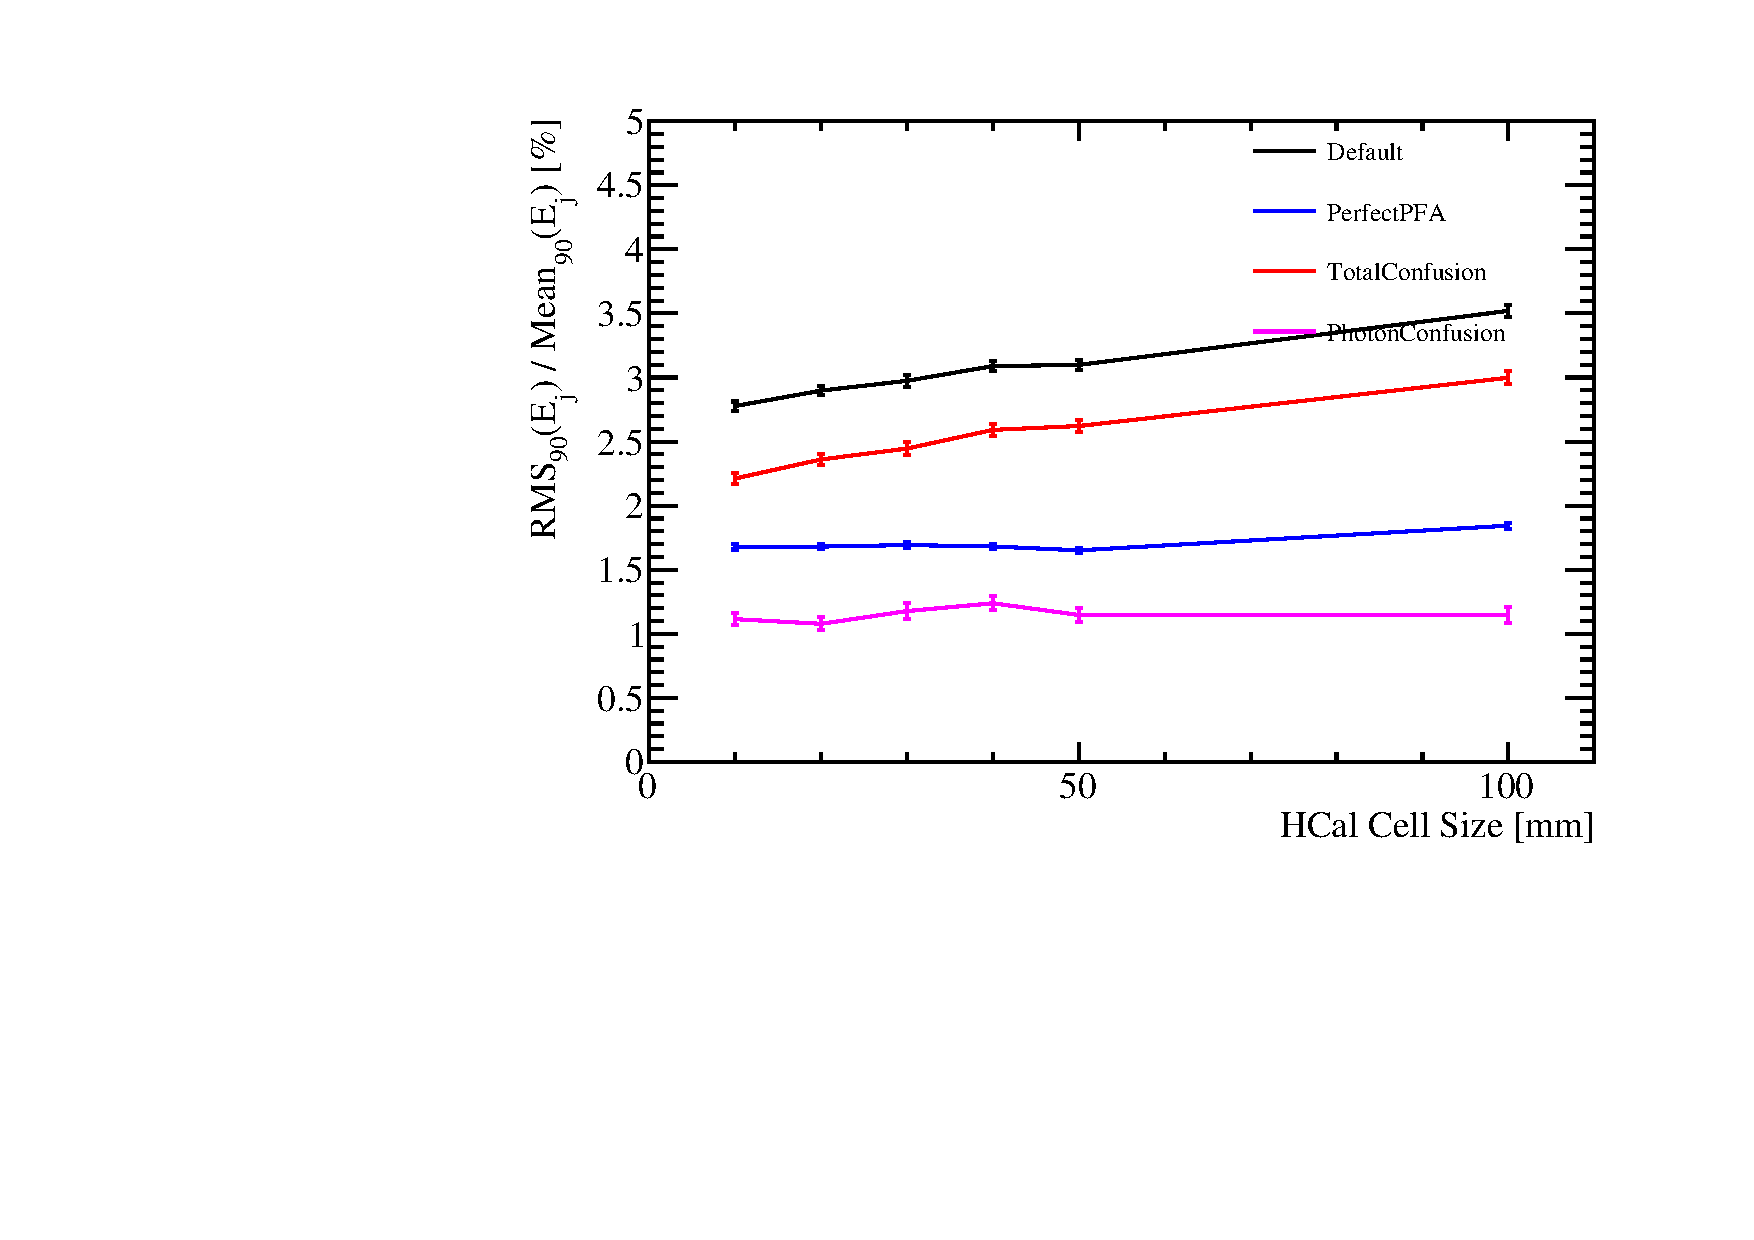
\includegraphics[width=0.5\textwidth]{OptimisationStudies/Plots/JetEnergyResolutions/JER_vs_HCalCellSize_500GeV_DiJet_Breakdown.pdf}}
\caption[Jet energy resolution breakdown as a function of HCal cell size for 45 and 250 GeV jets.]{Jet energy resolution breakdown as a function of HCal cell size for 45 and 250 GeV jets.}
\label{fig:hcalcellsizebreak}
\end{figure}

The jet energy resolution breakdowns, shown in figure, \ref{fig:hcalcellsizebreak}, show that the confusion term varies when changing the HCal cell size, but the intrinsic energy resolution does not.  Furthermore, the photon confusion is invariant to changes in HCal cell size, indicating that the observed overall performance changes are due to the effects of confusion arising from energy deposits from charged and neutral hadrons.  Once again for 45 GeV jets the detector performance is dominated by intrinsic energy resolution and so HCal cell size has little effect, while for 250 GeV jets the performance is dominated by confusion and HCal cell size becomes more significant.  

\begin{figure}
\centering
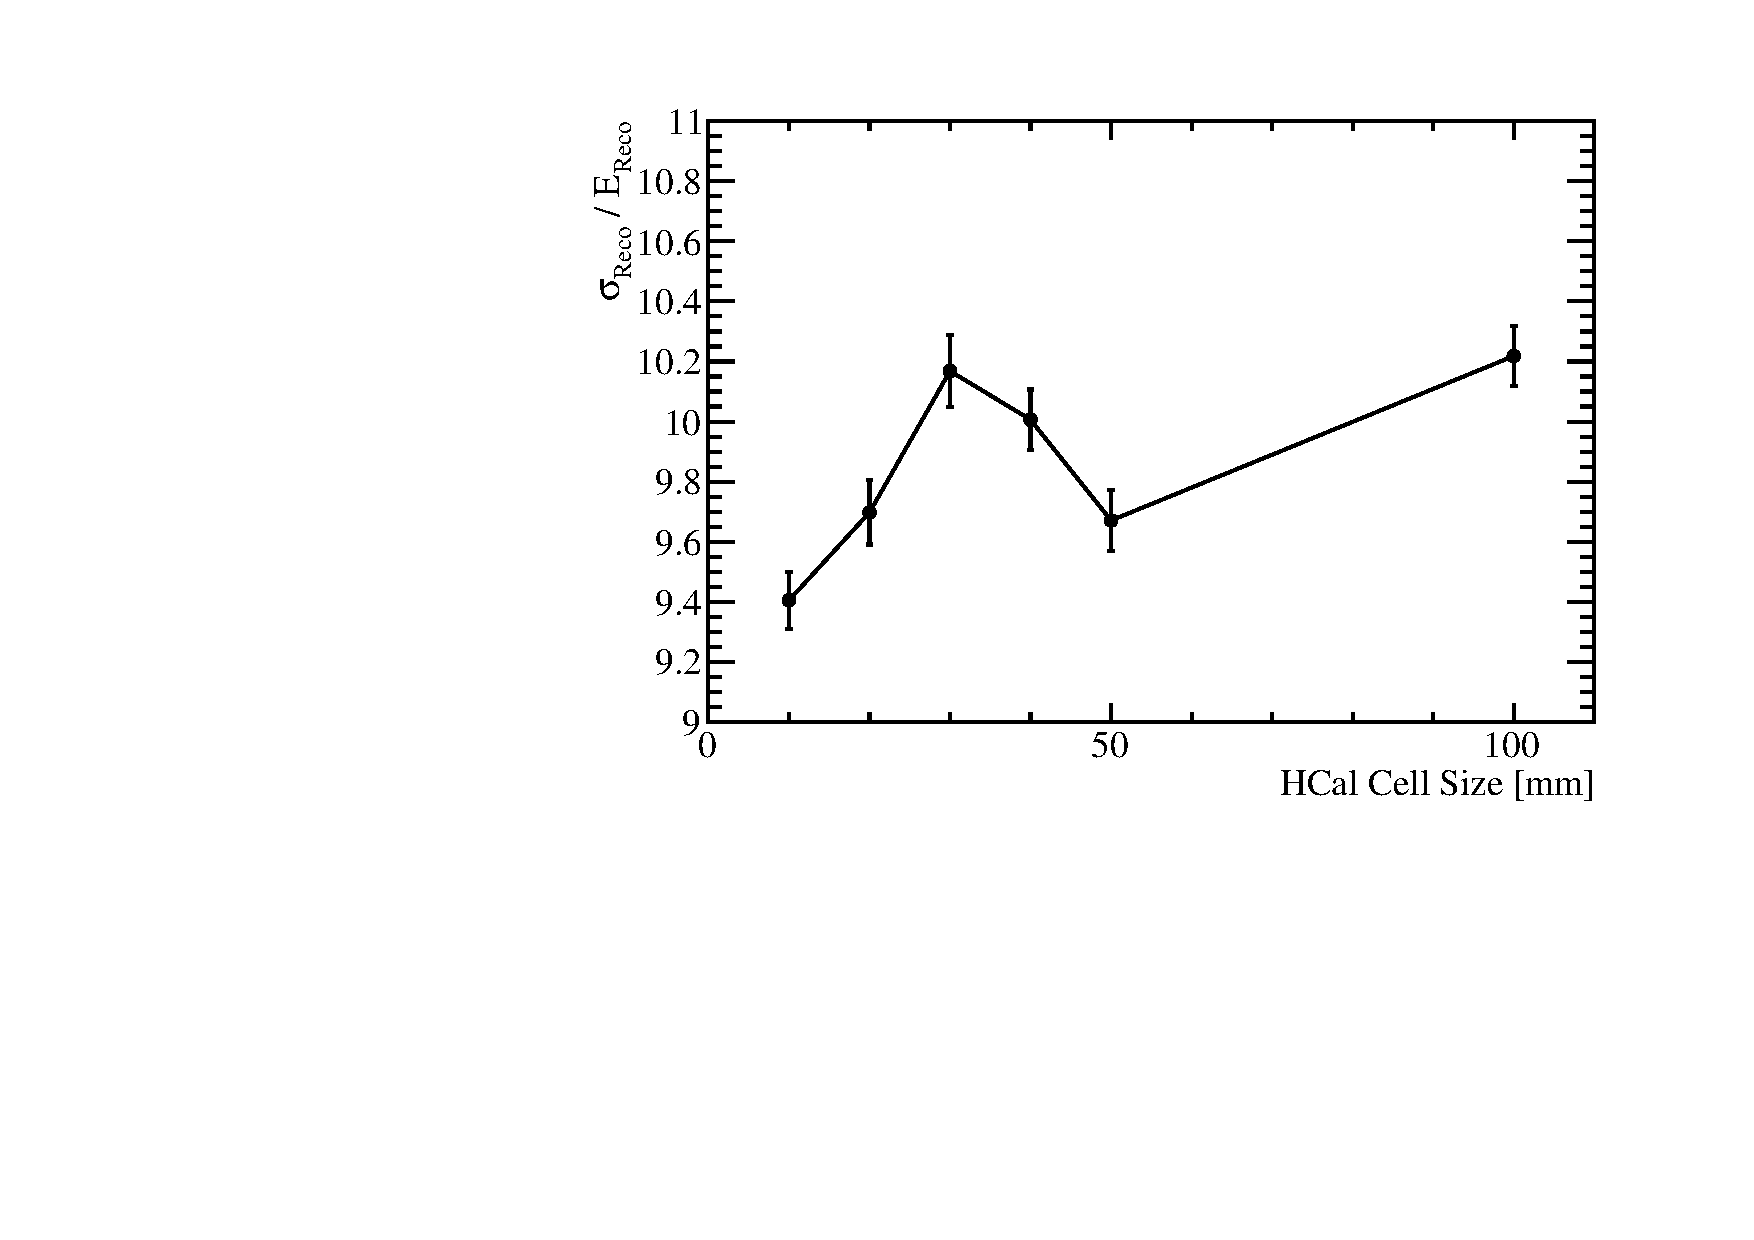
\includegraphics[width=0.5\textwidth]{OptimisationStudies/Plots/EnergyResolution/ER_vs_HCalCellSize_50GeVKaon0L.pdf}
\caption[Energy resolution as a function of HCal cell size for 50 GeV $\text{K}^{0}_{L}$.]{Energy resolution as a function of HCal cell size for 50 GeV $\text{K}^{0}_{L}$.}
\label{fig:hcalcellskaon}
\end{figure}

The energy resolution of single long lived neutral kaons, $\text{K}^{0}_{L}$, at 50 GeV is considered as a function of cell size in the HCal.  This is shown in figure \ref{fig:hcalcellskaon} and, as expected, the energy resolution of the detector is largely invariant to changes in the cell size in the HCal.  As these $\text{K}^{0}_{L}$ samples may deposit energy in the ECal, this figure represents the intrinsic energy resolution of the ILD detector as a whole and not purely that of the HCal.  However, it expected that the bulk of the energy deposited by these samples occurs within the HCal and so such plots are a useful representation of the HCal performance.  

The cell size of the HCal acts to determine the impact of confusion from charged and neutral hadron energy deposits.  It does not vary the intrinsic energy resolution of the detector, nor does it impact the reconstruction of photons.  As confusion is dominant at high jet energies the HCal cell size gains an increasing role in determining detector performance as the energy in an event increases. 

%========================================================================================

\subsection{HCal Number of Layers}
\label{sec:hcalnlayers}

This section focuses upon change in detector performance when varying the number of layers in the HCal.  For this study, the absorber and active layer thicknesses are not varied when adding or subtracting layers from the HCal, so both the total depth of the HCal as well as the number of sampling points of the hadronic showers varies simultaneously, this is in comparison to the study described in section \ref{sec:hcalsamplingfrequency} where the total depth of the HCal is fixed.  The detector models considered had 36, 42, 48, 54 and 60 layered HCals.  

\begin{figure}
\centering
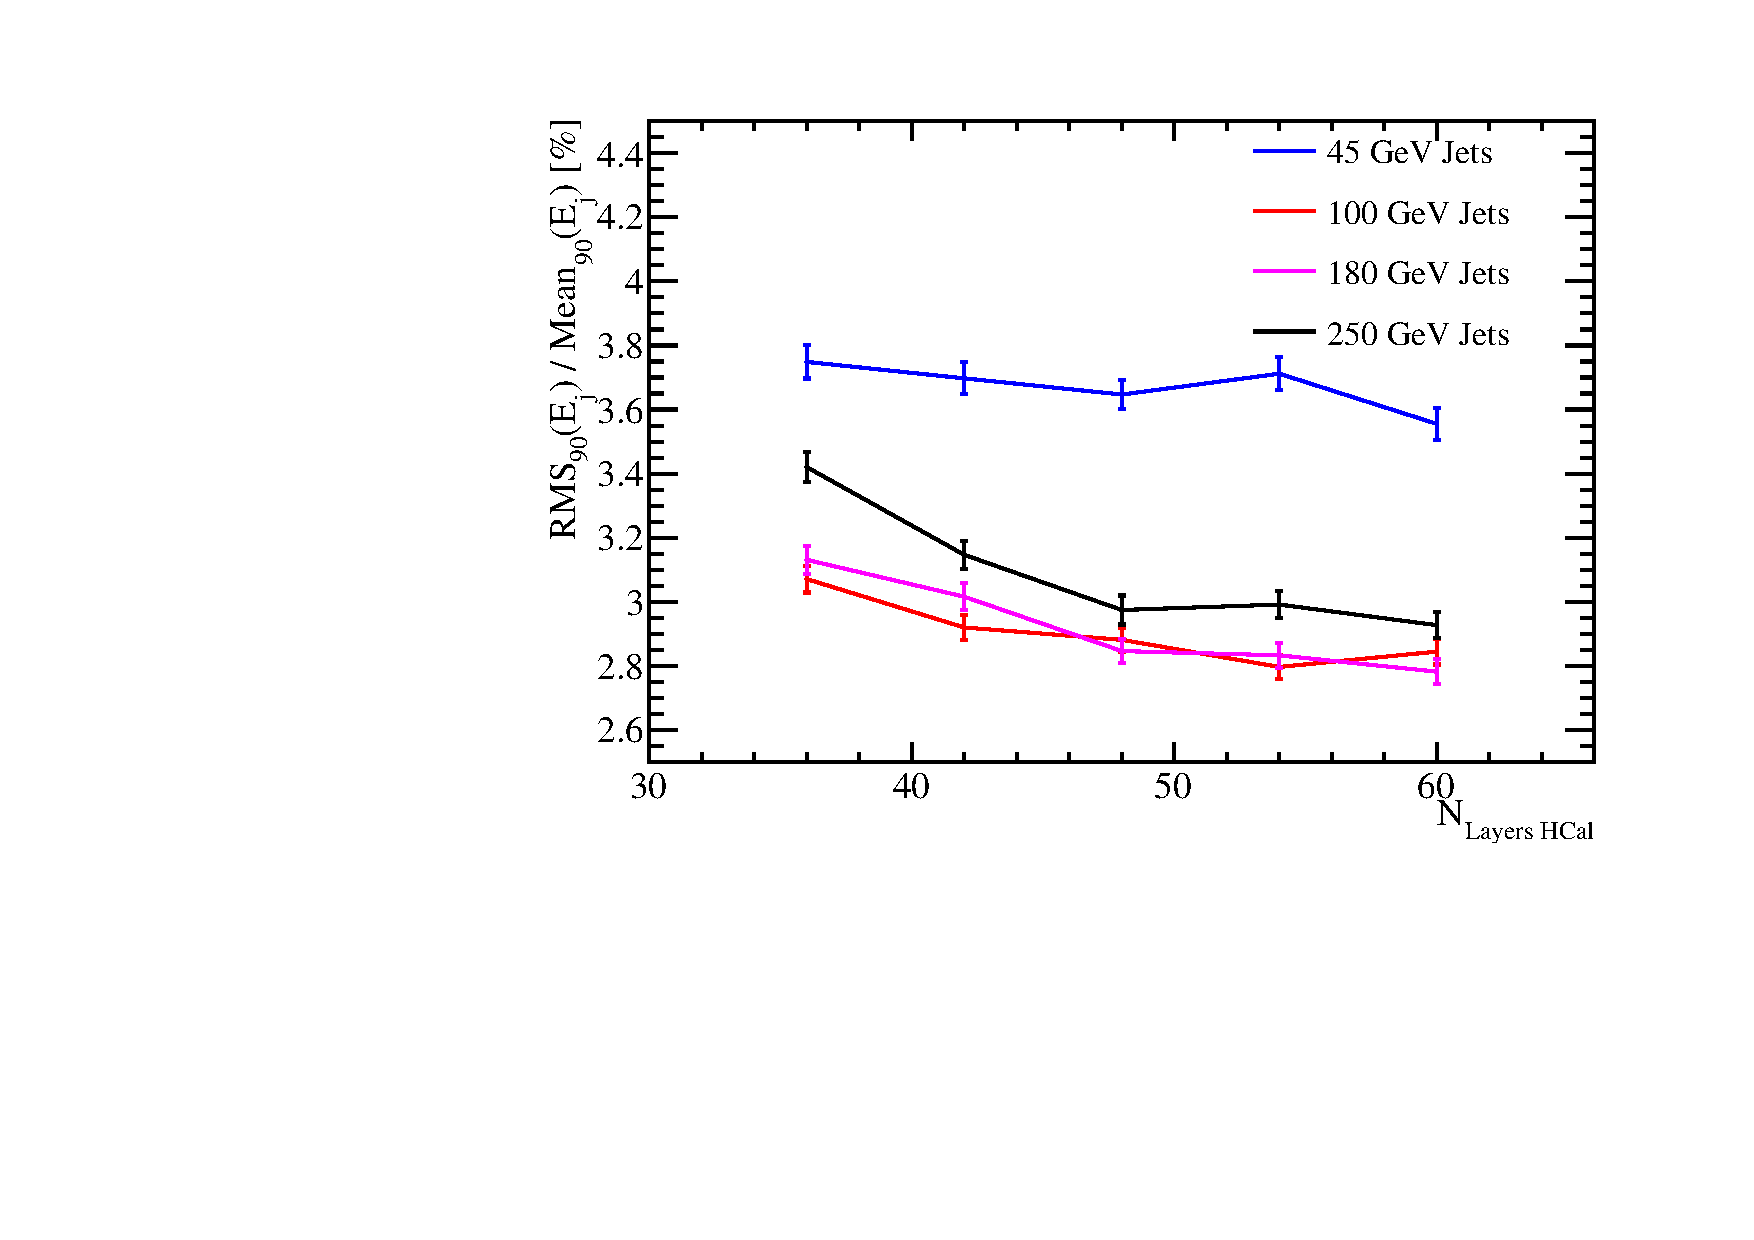
\includegraphics[width=0.5\textwidth]{OptimisationStudies/Plots/JetEnergyResolutions/JER_vs_NumberOfHCalLayersOfFixedDepth.pdf}
\caption[Jet energy resolution as a function of number of layers in the HCal.]{Jet energy resolution as a function of number of layers in the HCal.}
\label{fig:hcalnfixedlayers}
\end{figure}

The jet energy resolution for the various detector models considered is shown in figure \ref{fig:hcalnlayers}.  It was found that increasing the number of layers in the HCal improved the jet energy resolution for high energy jets, while for low energy jets no the performance change was observed.  The breakdown of the jet energy resolution for the high energy jets, shown in figure \ref{ig:hcalnfixedlayersbreak}, indicates a reduction in the confusion term is driving the change in performance when increasing the number of layers in the HCal.  

\begin{figure}
\centering
\subfloat[45 GeV Jets.]{\label{fig:hcalnlayers45break}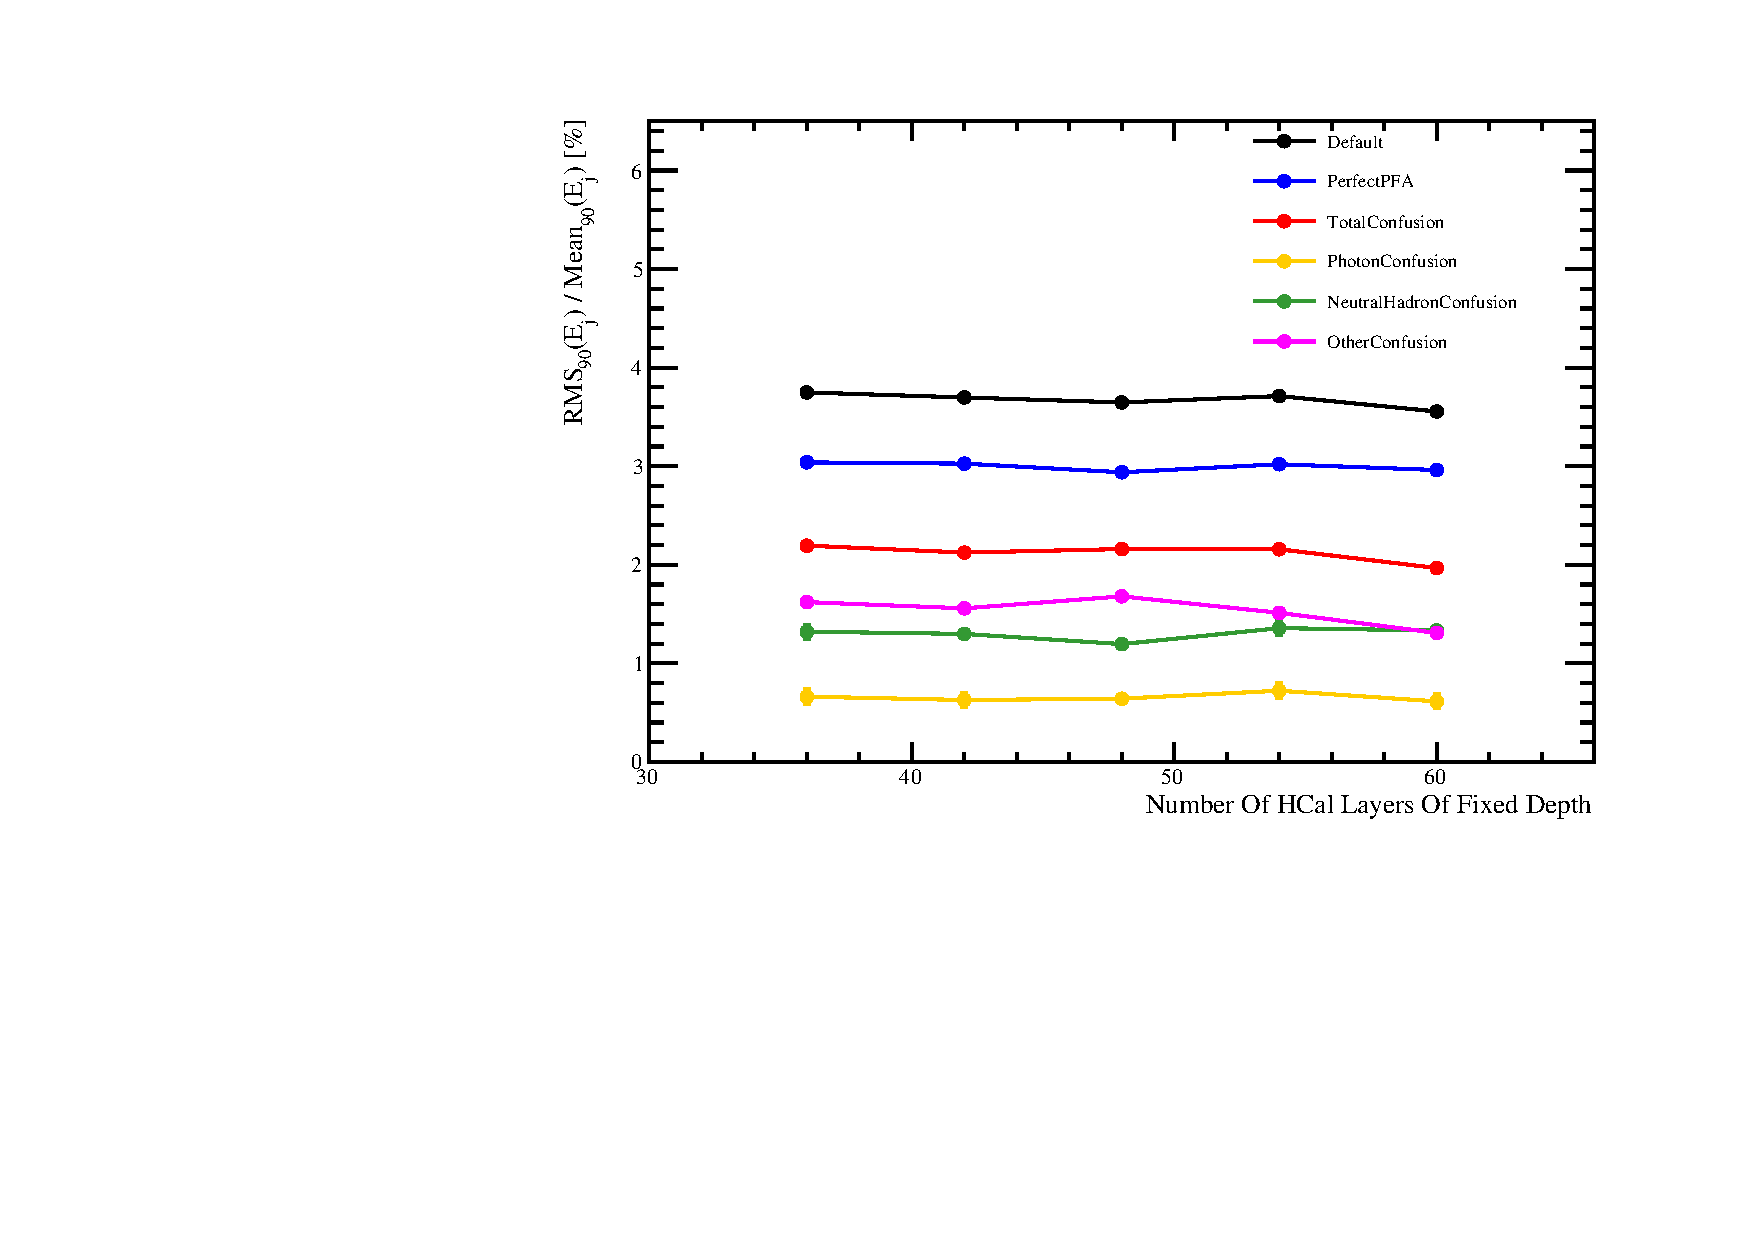
\includegraphics[width=0.5\textwidth]{OptimisationStudies/Plots/JetEnergyResolutions/JER_vs_NumberOfHCalLayersOfFixedDepth_91GeV_DiJet_Breakdown.pdf}}
\subfloat[250 GeV Jets.]{\label{fig:hcalnlayers250break}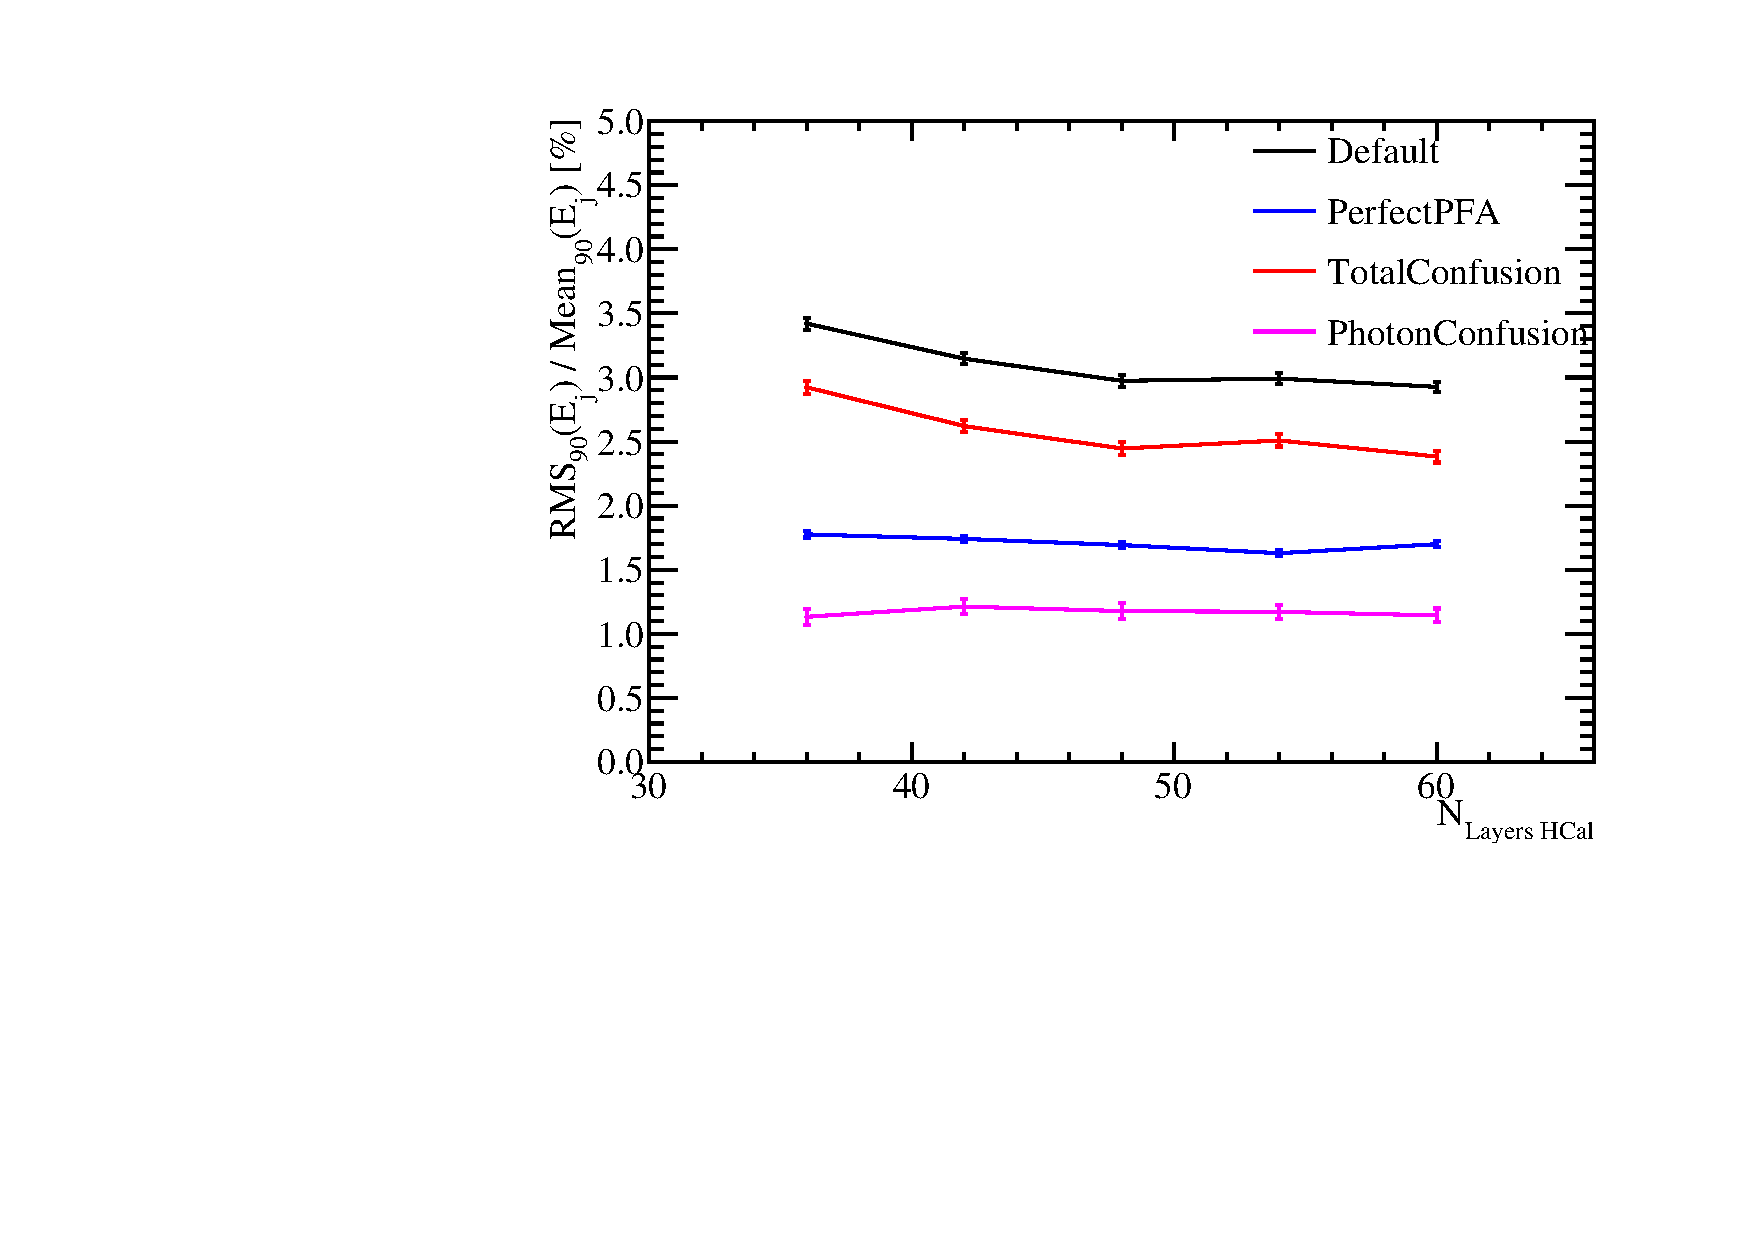
\includegraphics[width=0.5\textwidth]{OptimisationStudies/Plots/JetEnergyResolutions/JER_vs_NumberOfHCalLayersOfFixedDepth_500GeV_DiJet_Breakdown.pdf}}
\caption[Jet energy resolution breakdown as a function of number of layers in the HCal for 45 and 250 GeV jets.]{Jet energy resolution breakdown as a function of number of layers in the HCal for 45 and 250 GeV jets.}
\label{fig:hcalnfixedlayersbreak}
\end{figure}

While the intrinsic energy resolution for jets appeared largely invariant to changes in the number of layers in the HCal, it can be seen that there is an associated improvement in the energy resolution for neutral hadrons, which can be seen in figure \ref{fig:hcalnfixedlayerser}.  This change in neutral hadron energy resolution will be masked in the jet energy resolution study as only $\approx 10\%$ of the energy of a jet is carried in the form of neutral hadrons and the energy resolution change is minimal.   

\begin{figure}
\centering
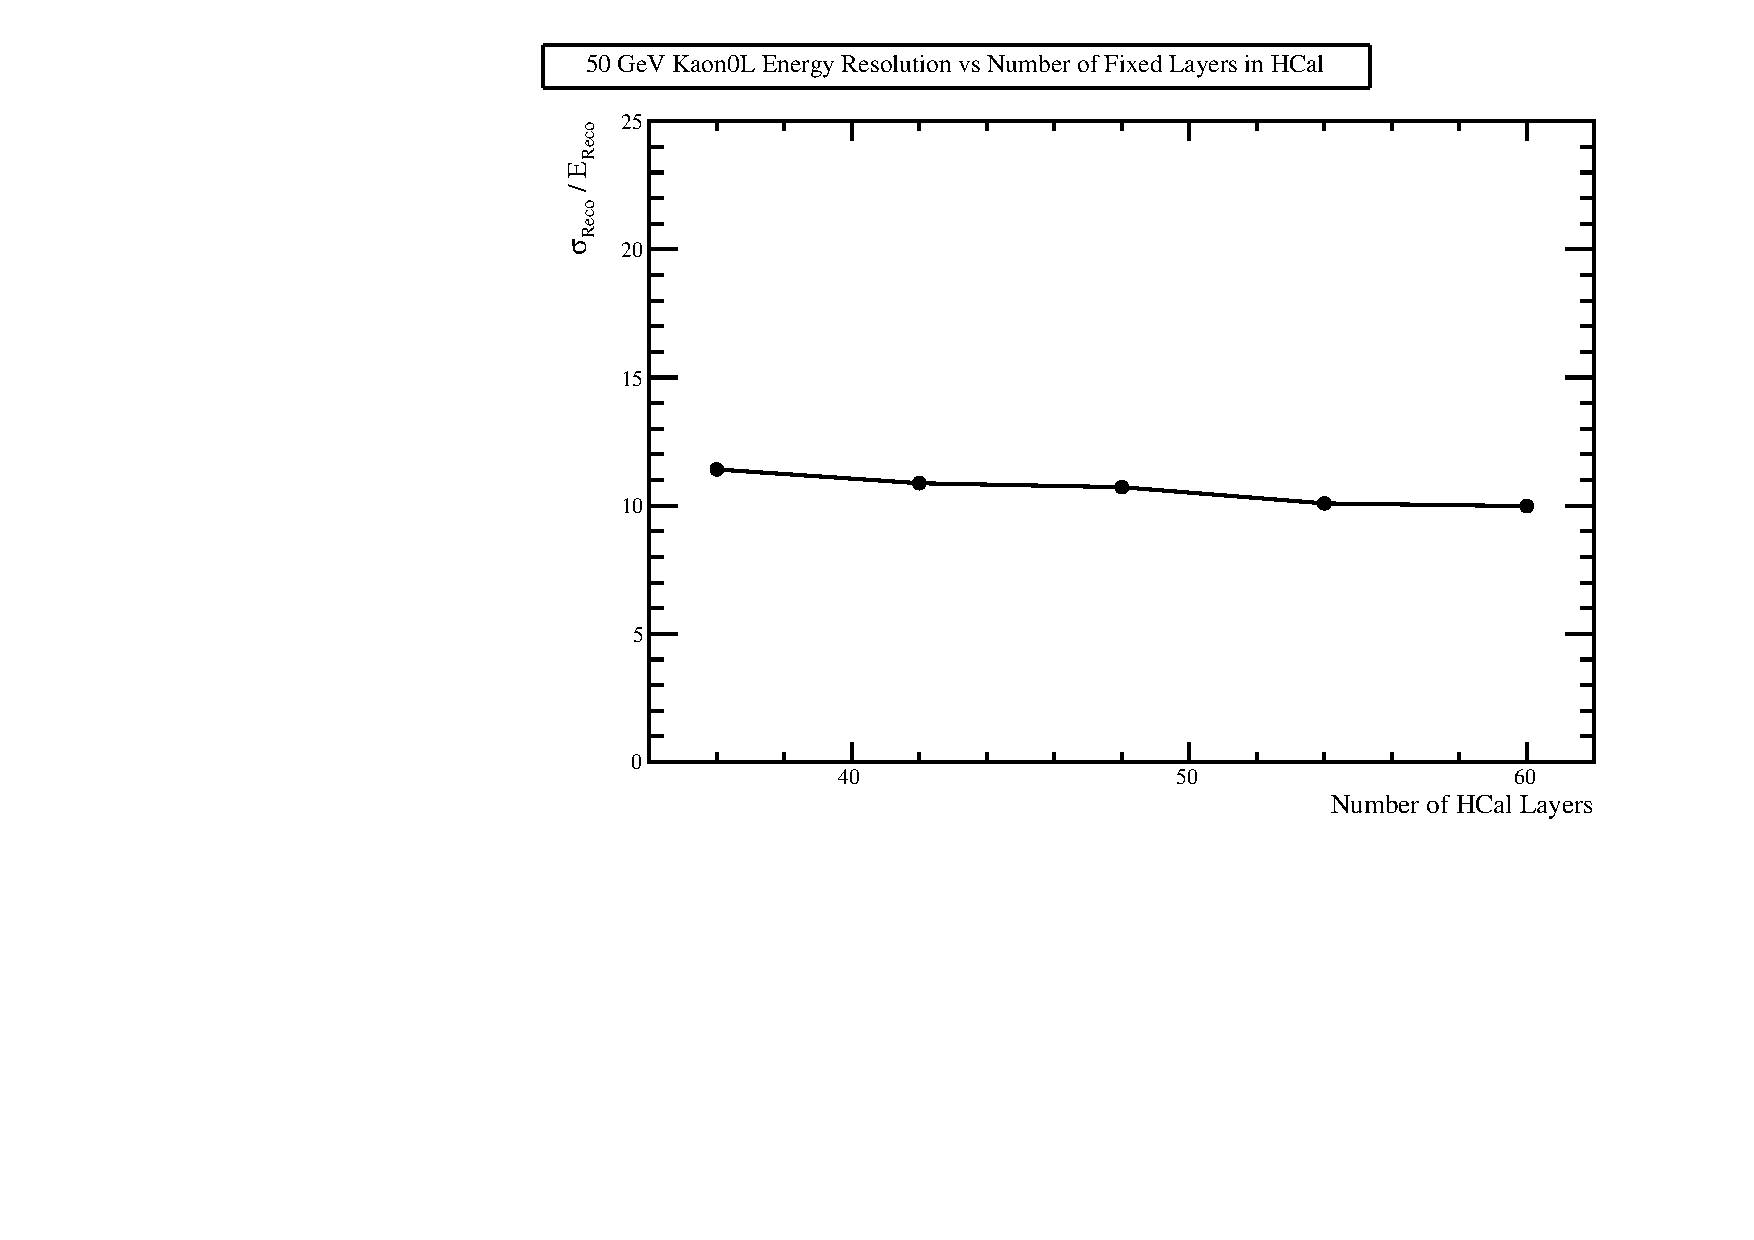
\includegraphics[width=0.5\textwidth]{OptimisationStudies/Plots/EnergyResolution/ER_vs_HCalNFixedLayers_50GeVKaon0L.pdf}
\caption[Energy resolution as a function of number of layers in the HCal for 50 GeV $\text{K}^{0}_{L}$.]{Energy resolution as a function of number of layers in the HCal  for 50 GeV $\text{K}^{0}_{L}$.}
\label{fig:hcalnfixedlayerser}
\end{figure}

In conclusion, a larger number of layers in the HCal is beneficial to detector performance both in terms of a reduction in pattern recognition confusion as well as an improvement in the energy resolution of neutral hadrons.  These performance changes at the energies considered are relatively small and so it would be feasible to consider changes to the nominal number of HCal layers.  However, at higher energies these conclusions could be significantly modified as leakage dominates.  

%========================================================================================

\subsection{HCal Sampling Fraction}
\label{sec:hcalsamplingfraction}
In this section the sampling fraction, the ratio of the active to absorber layer thicknesses were considered.  For all detector models considered in this section the total number of nuclear interaction lengths in the HCal was held constant, as was the number of layers in the HCal and the cell size.  The detector models considered are summarised in table \ref{table:hcalsamplingfraction}. 

\begin{table}[h!]
\centering
\begin{tabular}{ r r r }
\hline
Sampling Fraction & Absorber Thickness & Active Thickness \\
 & [mm] & [mm] \\
\hline
0.05 & 20.430 & 1.022 \\ 
0.10 & 20.213 & 2.021 \\
0.15 & 20.000 & 3.000 \\
0.20 & 19.792 & 3.958 \\
0.25 & 19.587 & 4.897 \\
\hline
\end{tabular}
\caption[Sampling fraction of HCal models considered.]{Sampling fraction of HCal models considered.}
\label{table:hcalsamplingfraction}
\end{table}

The jet energy resolution for these detector models is shown in figure \ref{fig:hcalnlayers}.  It was found that there is no significant change in performance when varying the sampling fraction.  

\begin{figure}
\centering
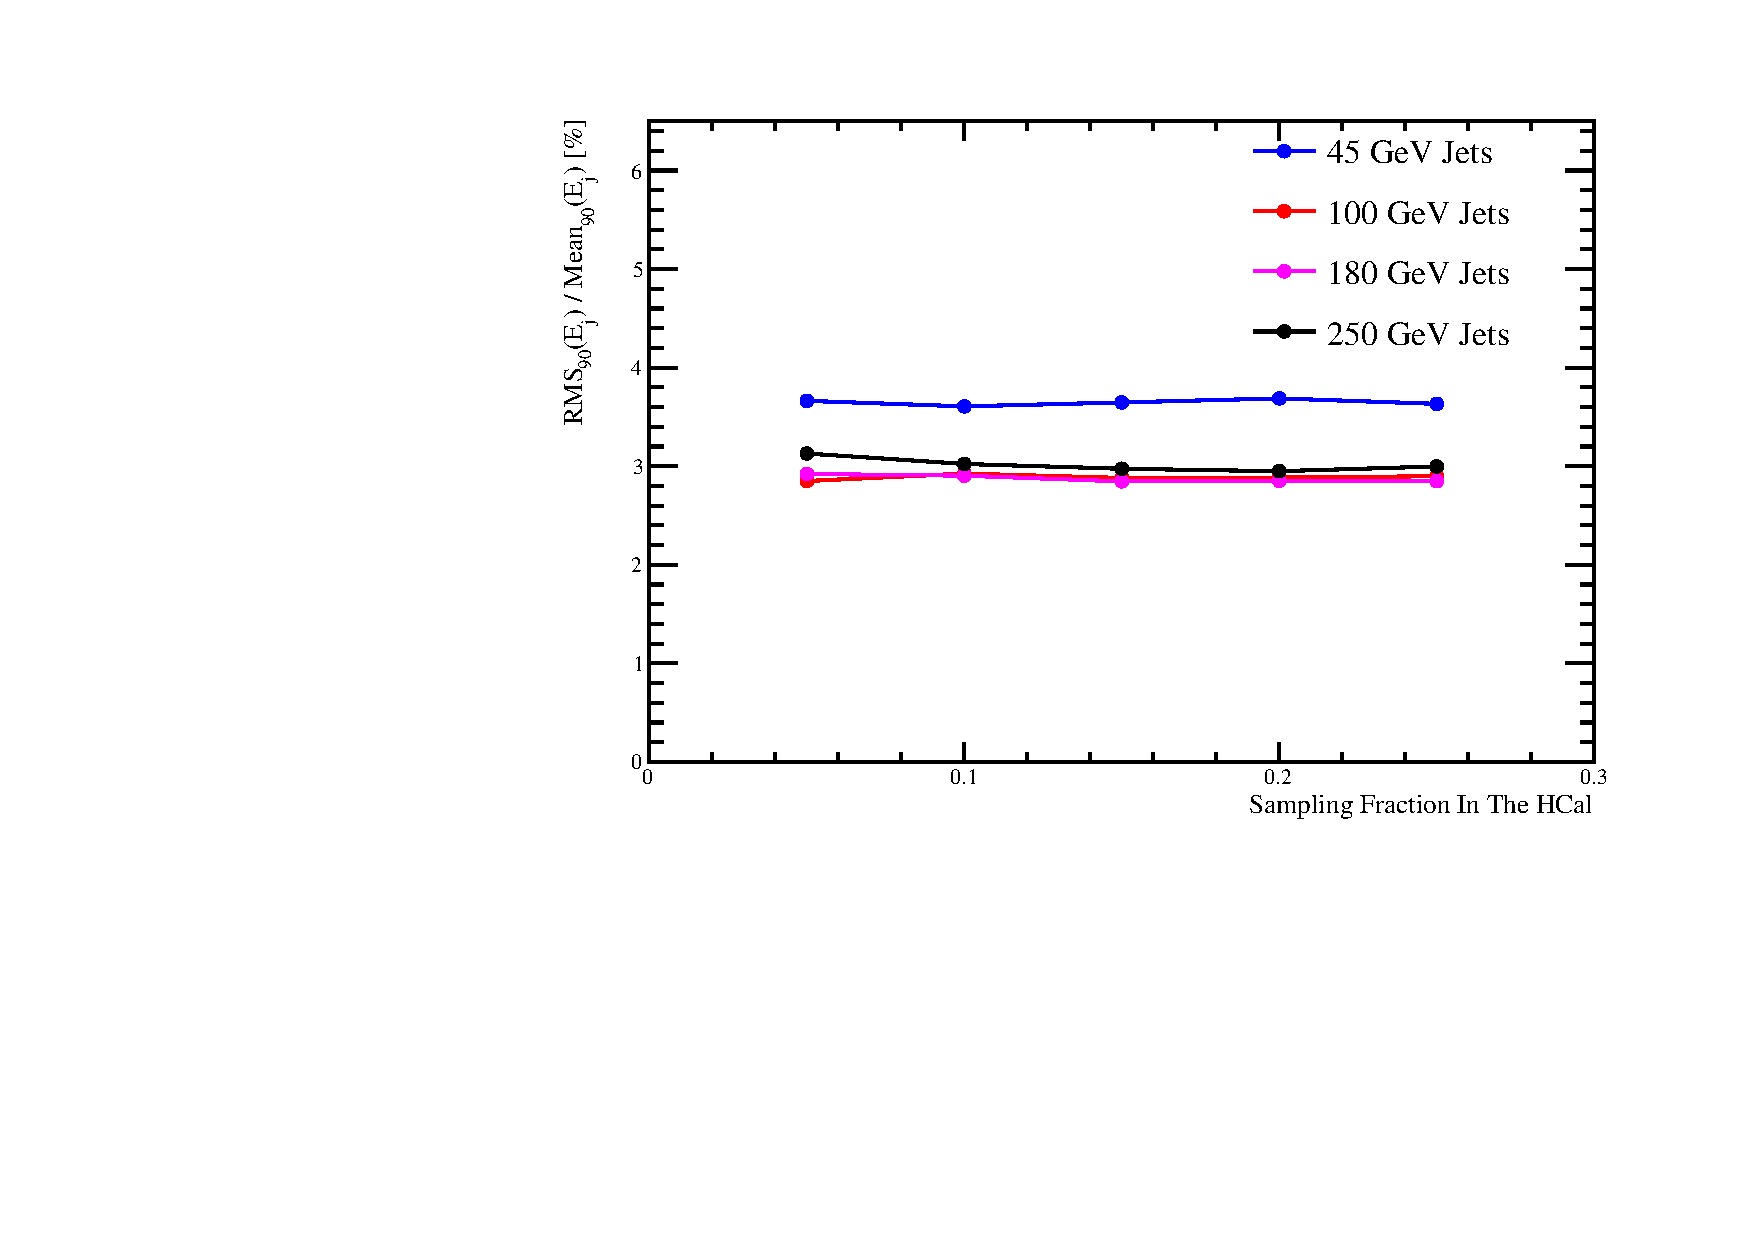
\includegraphics[width=0.5\textwidth]{OptimisationStudies/Plots/JetEnergyResolutions/JER_vs_SamplingFractionInTheHCal.pdf}
\caption[Jet energy resolution as a function of sampling frequency in the HCal.]{Jet energy resolution as a function of sampling frequency in the HCal.  Label needs fixing.}
\label{fig:hcalsamplingfraction}
\end{figure}

%========================================================================================

\subsection{HCal Sampling Frequency}
\label{sec:hcalsamplingfrequency}
This section aims to determine the change in performance when the sampling frequency, the number of times a particle shower is sampled per unit length, in the HCal is varied.  This was done by varying the number of readout layers, while maintaining the total number of nuclear interaction lengths contained within the HCal.  In all cases the absorber material was steel while the active material was scintillator.  Each HCal configuration had the same total number of nuclear interaction lengths, 5.72 $\lambda_{I}$ in the absorber material and 0.19 $\lambda_{I}$ in the active material, however, the thickness of the layers was varied depending on the total number of layers being considered.  The ratio of the active material layers to the absorber material layers, the sampling fraction, was also kept constant in this study.  A summary of the detector models considered in this study can be found in table \ref{table:nlayershcaloption}.  

\begin{table}[h!]
\centering
\begin{tabular}{ l l l }
\hline
Number $N_{\text{Layers HCal}}$& Absorber Thickness & Active Thickness \\
 & [mm] & [mm] \\
\hline
60 & 16.00 & 2.40 \\ 
54 & 17.78 & 2.67 \\
48 & 20.00 & 3.00 \\
42 & 22.86 & 3.43 \\
36 & 26.67 & 4.00 \\
30 & 32.00 & 4.80 \\
24 & 40.00 & 6.00 \\
18 & 53.33 & 8.00 \\
\hline
\end{tabular}
\caption[Cell size layout of various HCal models considered.]{Cell size layout of various HCal models considered.}
\label{table:nlayershcaloption}
\end{table}

\begin{figure}
\centering
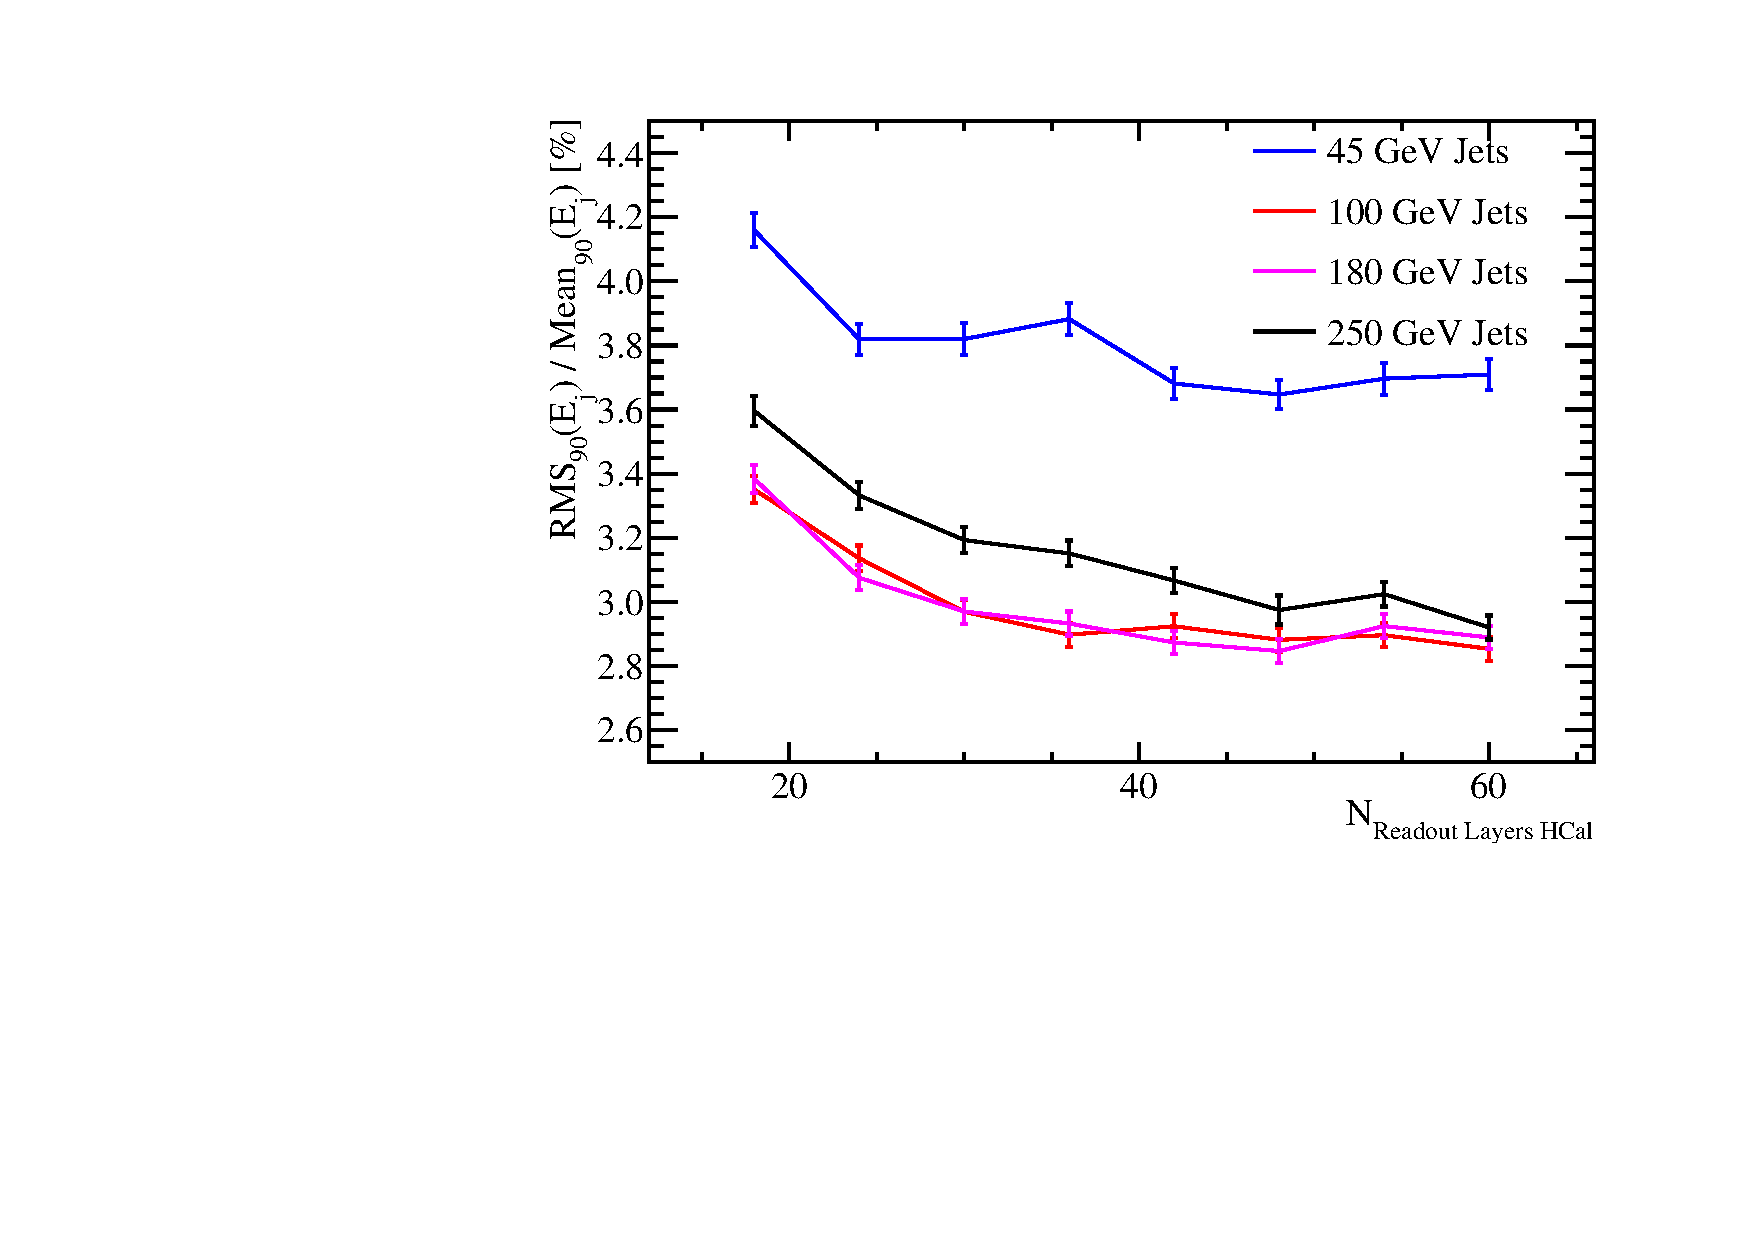
\includegraphics[width=0.5\textwidth]{OptimisationStudies/Plots/JetEnergyResolutions/JER_vs_NumberOfLayersInTheHCal.pdf}
\caption[Jet energy resolution as a function of sampling frequency in the HCal.]{Jet energy resolution as a function of sampling frequency in the HCal.}
\label{fig:hcalnlayers}
\end{figure}

The jet energy resolution for the various detector models considered is shown in figure \ref{fig:hcalnlayers}.  It was found that increasing the number of layers in the HCal, for the same total thickness, improved the jet energy resolution for all jet energies considered.  Based on the increase in the frequency of sampling of particle showers in the HCal, it is expected that the intrinsic energy resolution of the detector should improve.  However, the improvement observed in jet energy resolution for high energy jets indicates that sampling frequency is also affecting the confusion terms.

\begin{figure}
\centering
\subfloat[45 GeV Jets.]{\label{fig:hcalnlayers45break}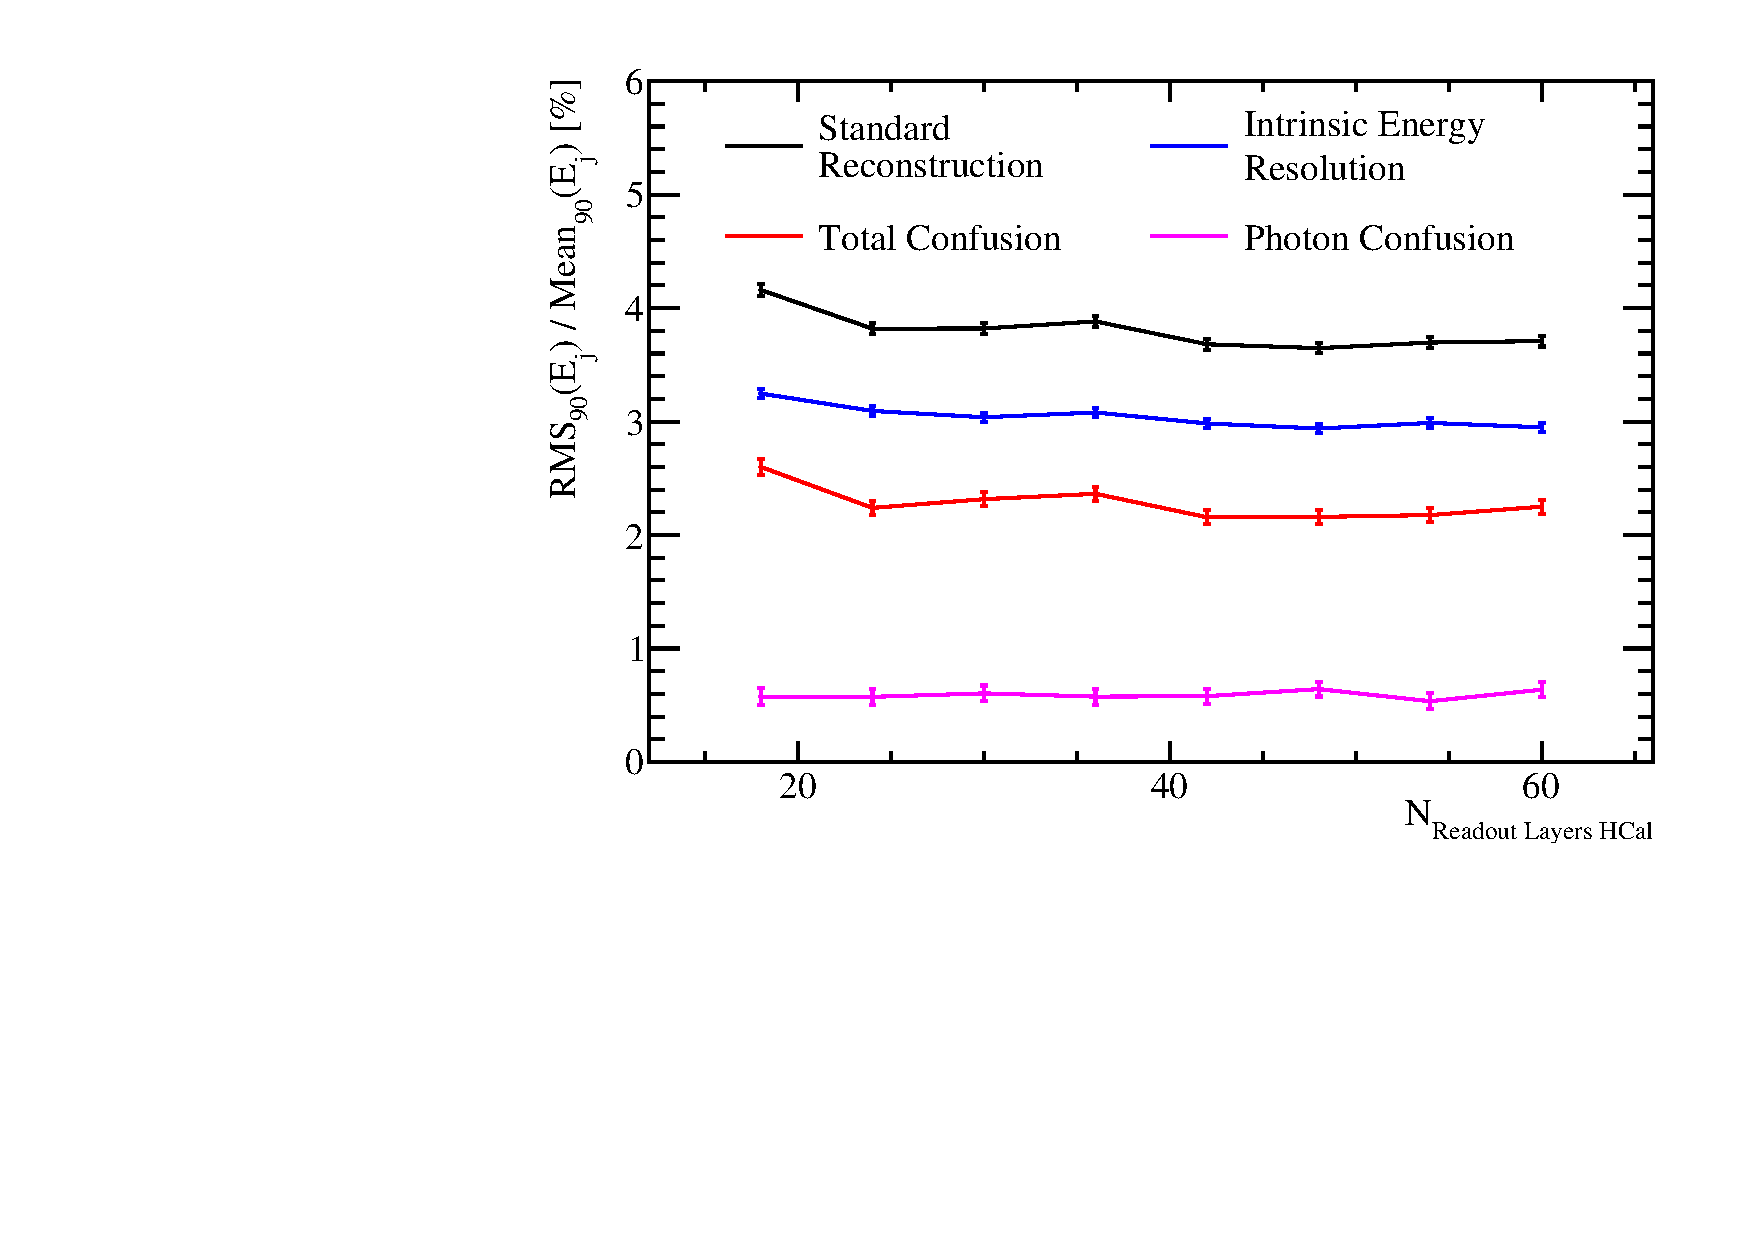
\includegraphics[width=0.5\textwidth]{OptimisationStudies/Plots/JetEnergyResolutions/JER_vs_NumberOfLayersInTheHCal_91GeV_DiJet_Breakdown.pdf}}
\subfloat[250 GeV Jets.]{\label{fig:hcalnlayers250break}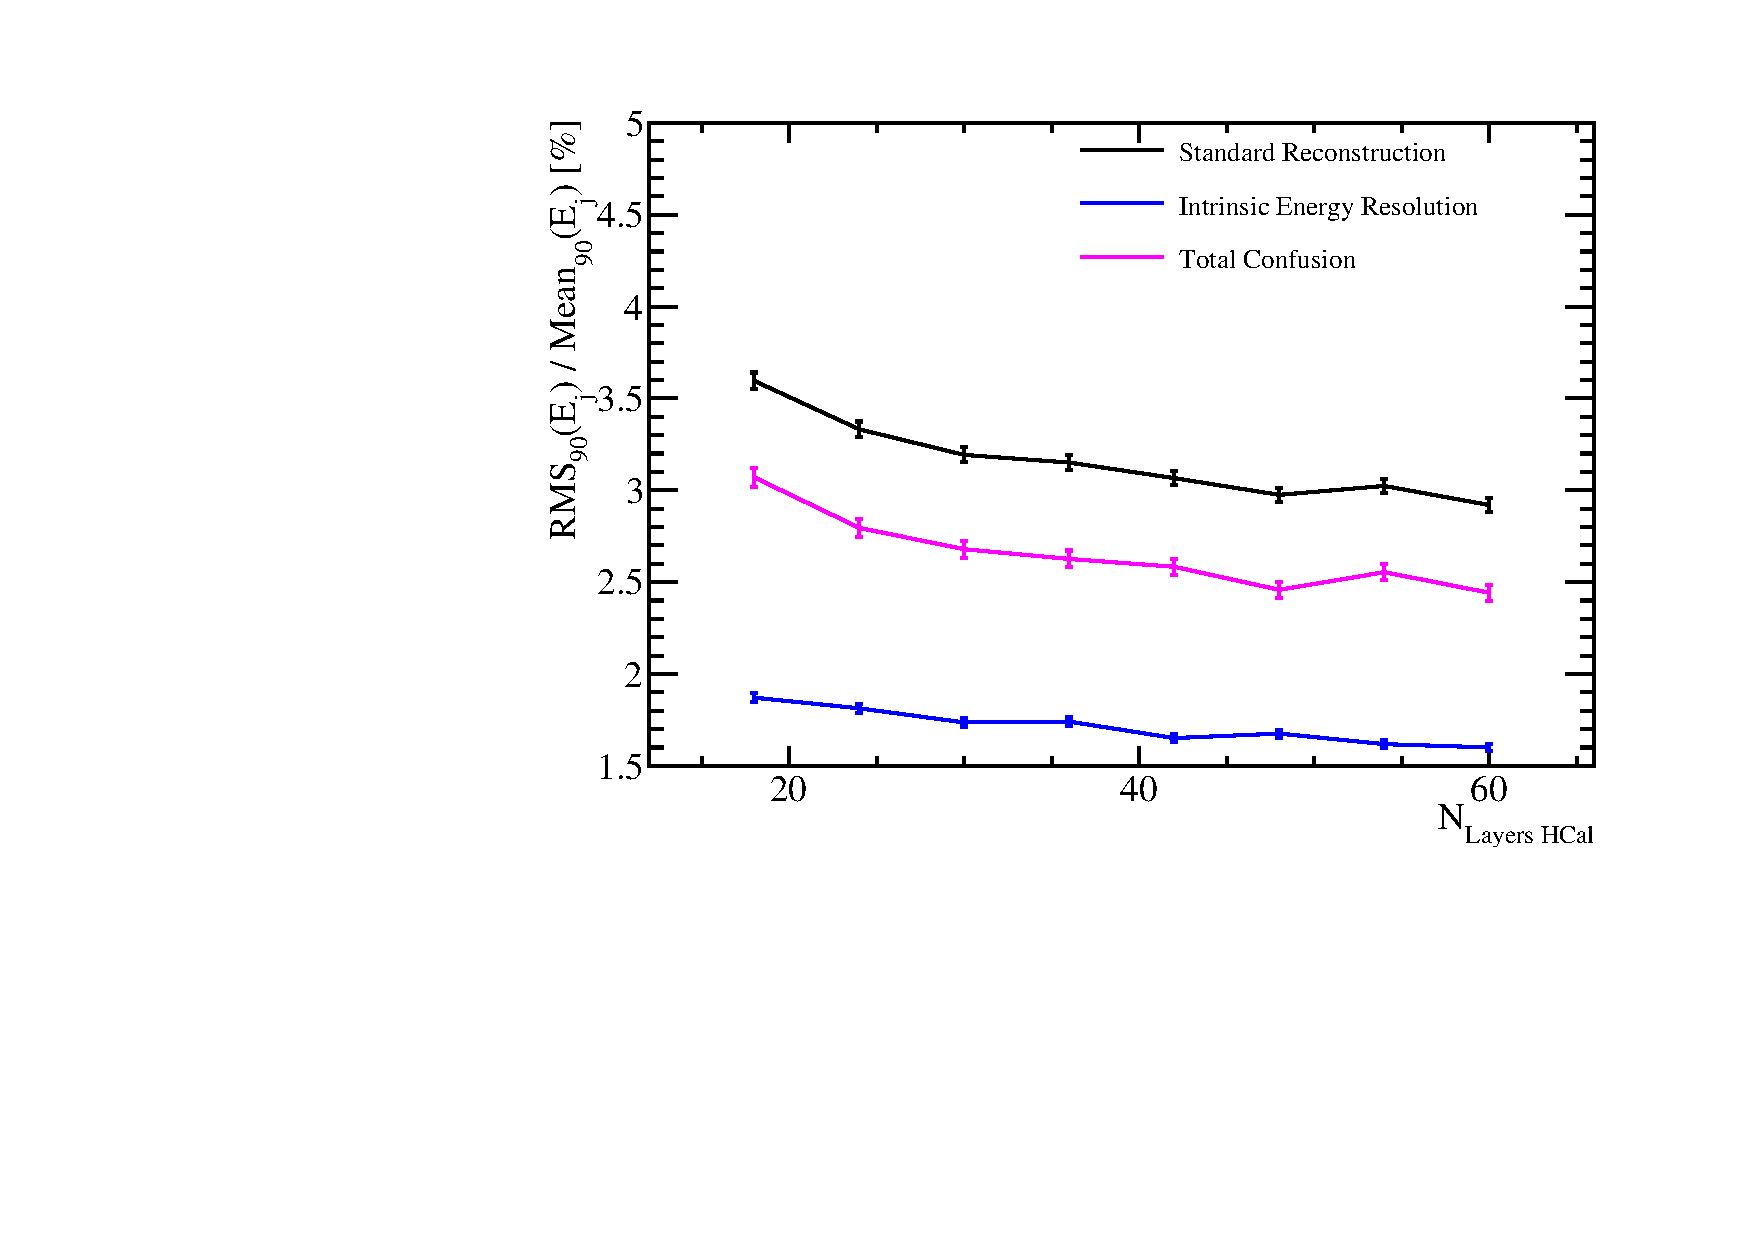
\includegraphics[width=0.5\textwidth]{OptimisationStudies/Plots/JetEnergyResolutions/JER_vs_NumberOfLayersInTheHCal_500GeV_DiJet_Breakdown.pdf}}
\caption[Jet energy resolution breakdown as a function of HCal sampling frequency for 45 and 250 GeV jets.]{Jet energy resolution breakdown as a function of HCal sampling frequency for 45 and 250 GeV jets.}
\label{fig:hcalnlayersbreak}
\end{figure}

These trends are further explored by considering the breakdown of jet energy resolution, which are shown in figure \ref{fig:hcalnlayersbreak}.  As expected from the standard performance reconstruction trends as a function of jet energy, there is an improvement in both the intrinsic energy resolution and a reduction in the impact of confusion when the number of layers in the HCal is increased.  The dominant trend driving the overall detector performance is that associated with the confusion of separating energy deposits from charged and neutral particles.  This emphasises the importance of pattern recognition to detector performance in the particle flow paradigm.    

\begin{figure}
\centering
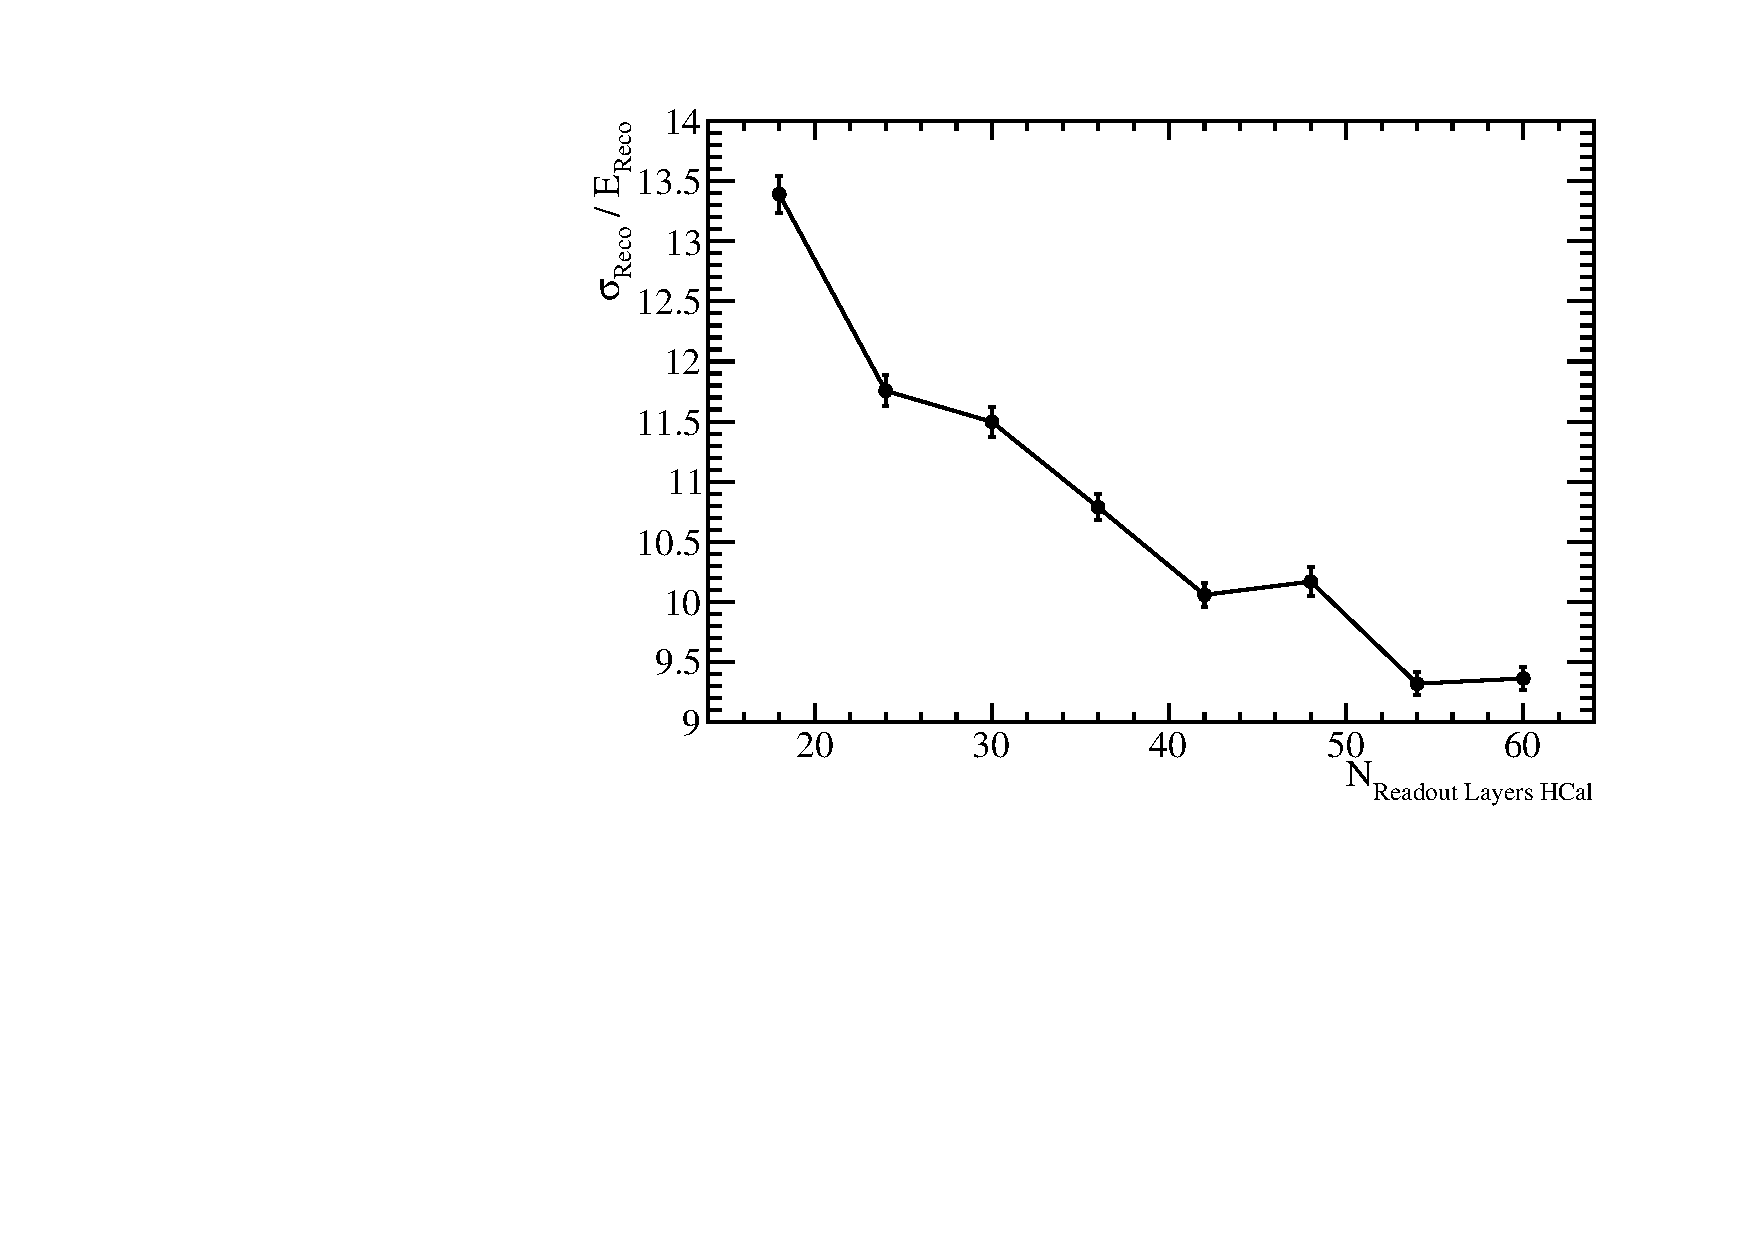
\includegraphics[width=0.5\textwidth]{OptimisationStudies/Plots/EnergyResolution/ER_vs_NHCalVariableLayers_50GeVKaon0L.pdf}
\caption[Energy resolution as a function of HCal sampling frequency for 50 GeV $\text{K}^{0}_{L}$.]{Energy resolution as a function of HCal sampling frequency for 50 GeV $\text{K}^{0}_{L}$.}
\label{fig:hcalnlayers}
\end{figure}

The change in the intrinsic energy resolution of the HCal when varying the sampling frequency is best summarised by looking at the energy resolution of neutral hadrons.  A plot of energy resolution against the number of readout layers in the HCal for 50 GeV $\text{K}^{0}_{L}$ can be found in figure \ref{fig:hcalnlayers}.  This data shows that a reduction in sampling frequency of a particle shower that accompanies a reduction in the number of readout layers results in a broadening of energy distributions and a degradation in the resolution.  It should again be emphasised that these results are for the full ILD detector model and so include the effect of the $\approx 1 \lambda_{I}$ in the ECal.  

The increasing the HCal sampling frequency has a twofold effect on the detector performance: an increase in sampling rate of particle showers and an improvement to the intrinsic energy resolution and a reduction in the confusion arising from associating energy deposits from hadrons.  

%========================================================================================
%========================================================================================

\section{Global Detector Parameters}
This section focuses upon optimisation of two global detector parameters; the magnetic field strength and the ECal inner radius.  While these are not directly related to the calorimeter they will both effect detector performance and so were deemed worthy of study alongside the calorimeter parameters. 

%========================================================================================

\subsection{The Magnetic Field Strength}
\label{sec:bfield}
The magnetic field is vital to the successful application of particle flow calorimetry.  Any charged particles passing through the detector transverse helices that, once reconstructed, can be fitted to give the momentum and so energy of said particle in the particle flow paradigm.  The magnetic field also created a separation between charged and neutral hadrons energy deposits in the calorimeters.  The larger the magnetic field, the greater this separation and the easier to avoid confusion associate tracks to the correct energy deposits in the calorimeters, which is crucial for particle flow.

\begin{figure}
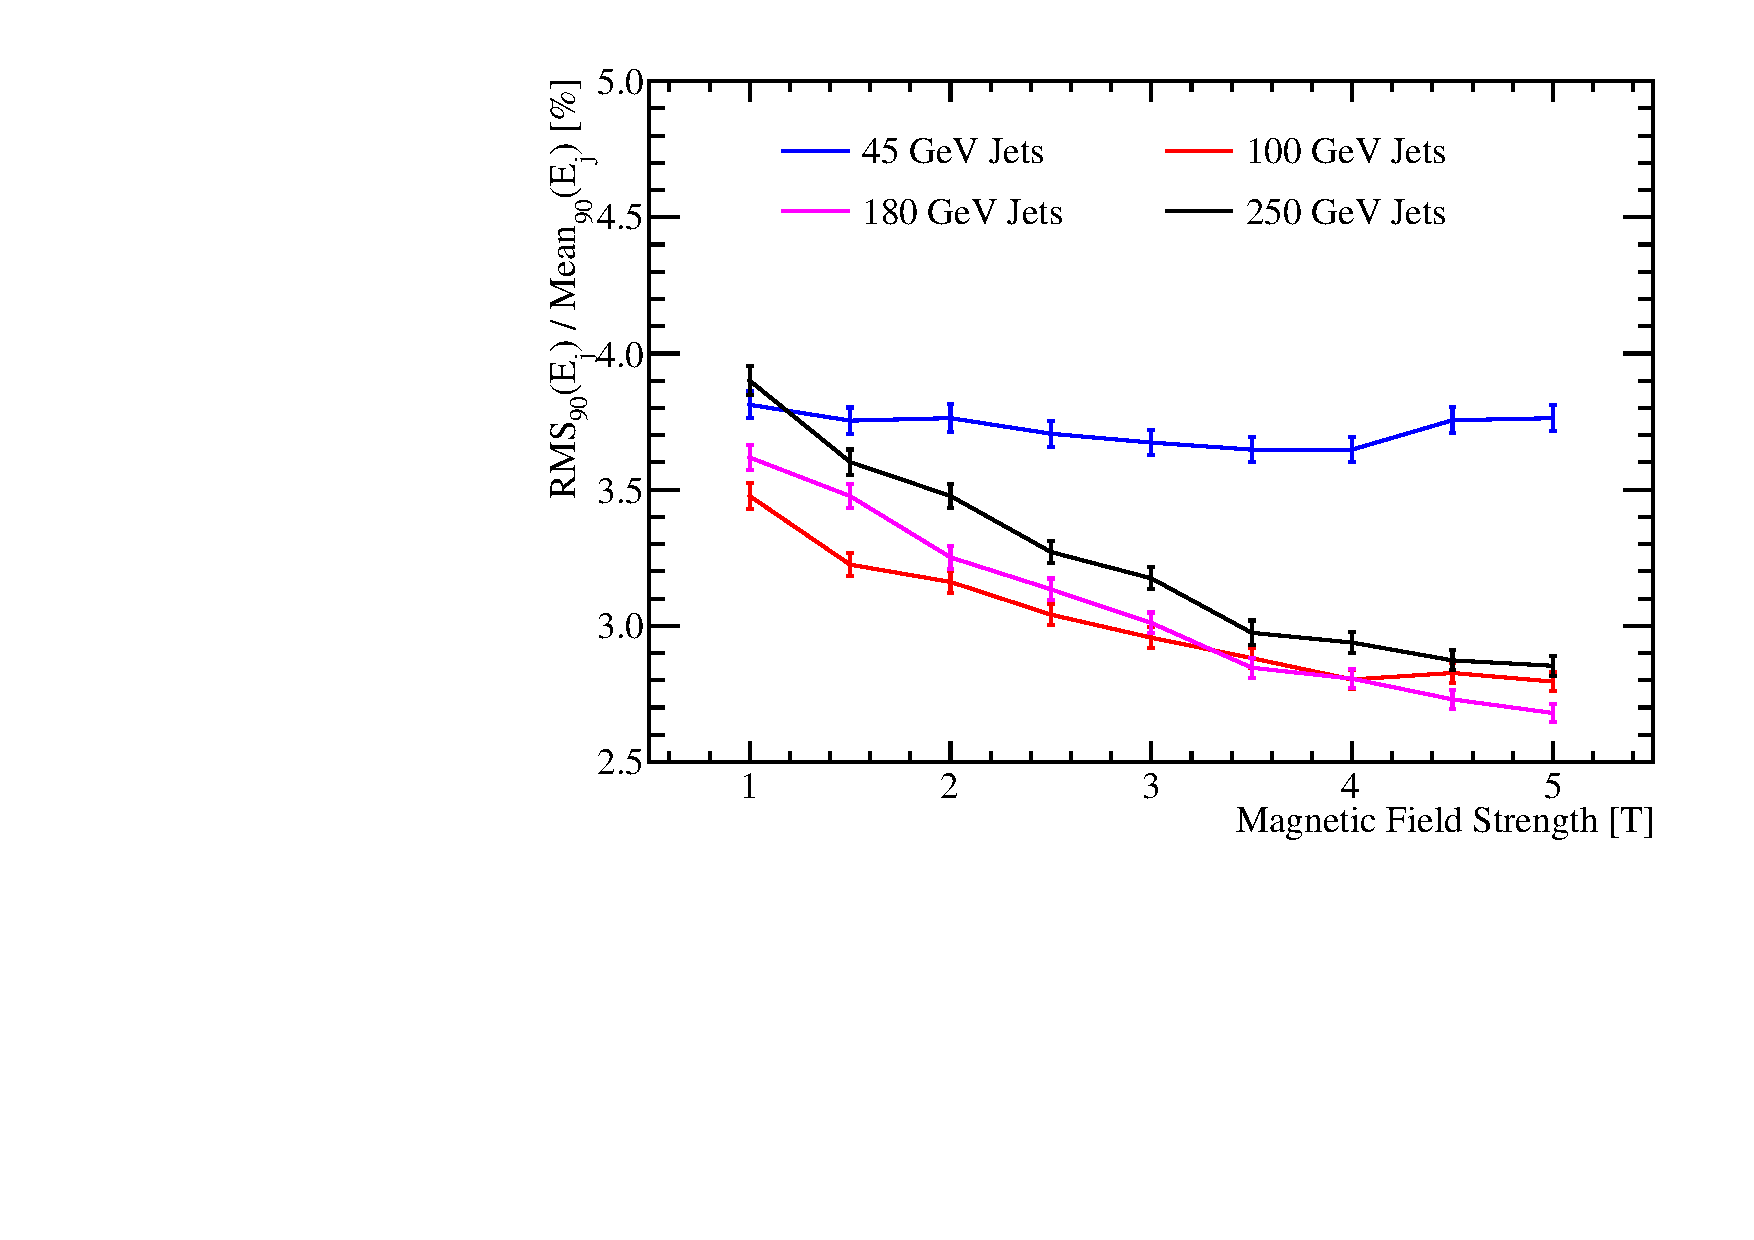
\includegraphics[width=0.5\textwidth]{OptimisationStudies/Plots/JetEnergyResolutions/JER_vs_MagneticFieldStrength.pdf}
\caption[Jet energy resolution as a function of magnetic field strength.]{Jet energy resolution is shown for several fixed energy jets as a function of magnetic field strength.}
\label{fig:bfield}
\end{figure}

The magnetic field strengths considered in this study ranged from 1 to 5 T in steps of 0.5 T.  The jet energy resolutions as a function of magnetic field strength, shown in figure \ref{fig:bfield}, shows that the jet energy resolution decreases with increasing magnetic field strength for high energy jets.  At low energies the performance is largely invariant to magnetic field strength.  

\begin{figure}
\subfloat[45 GeV Jets.]{\label{fig:hcalnlayers45break}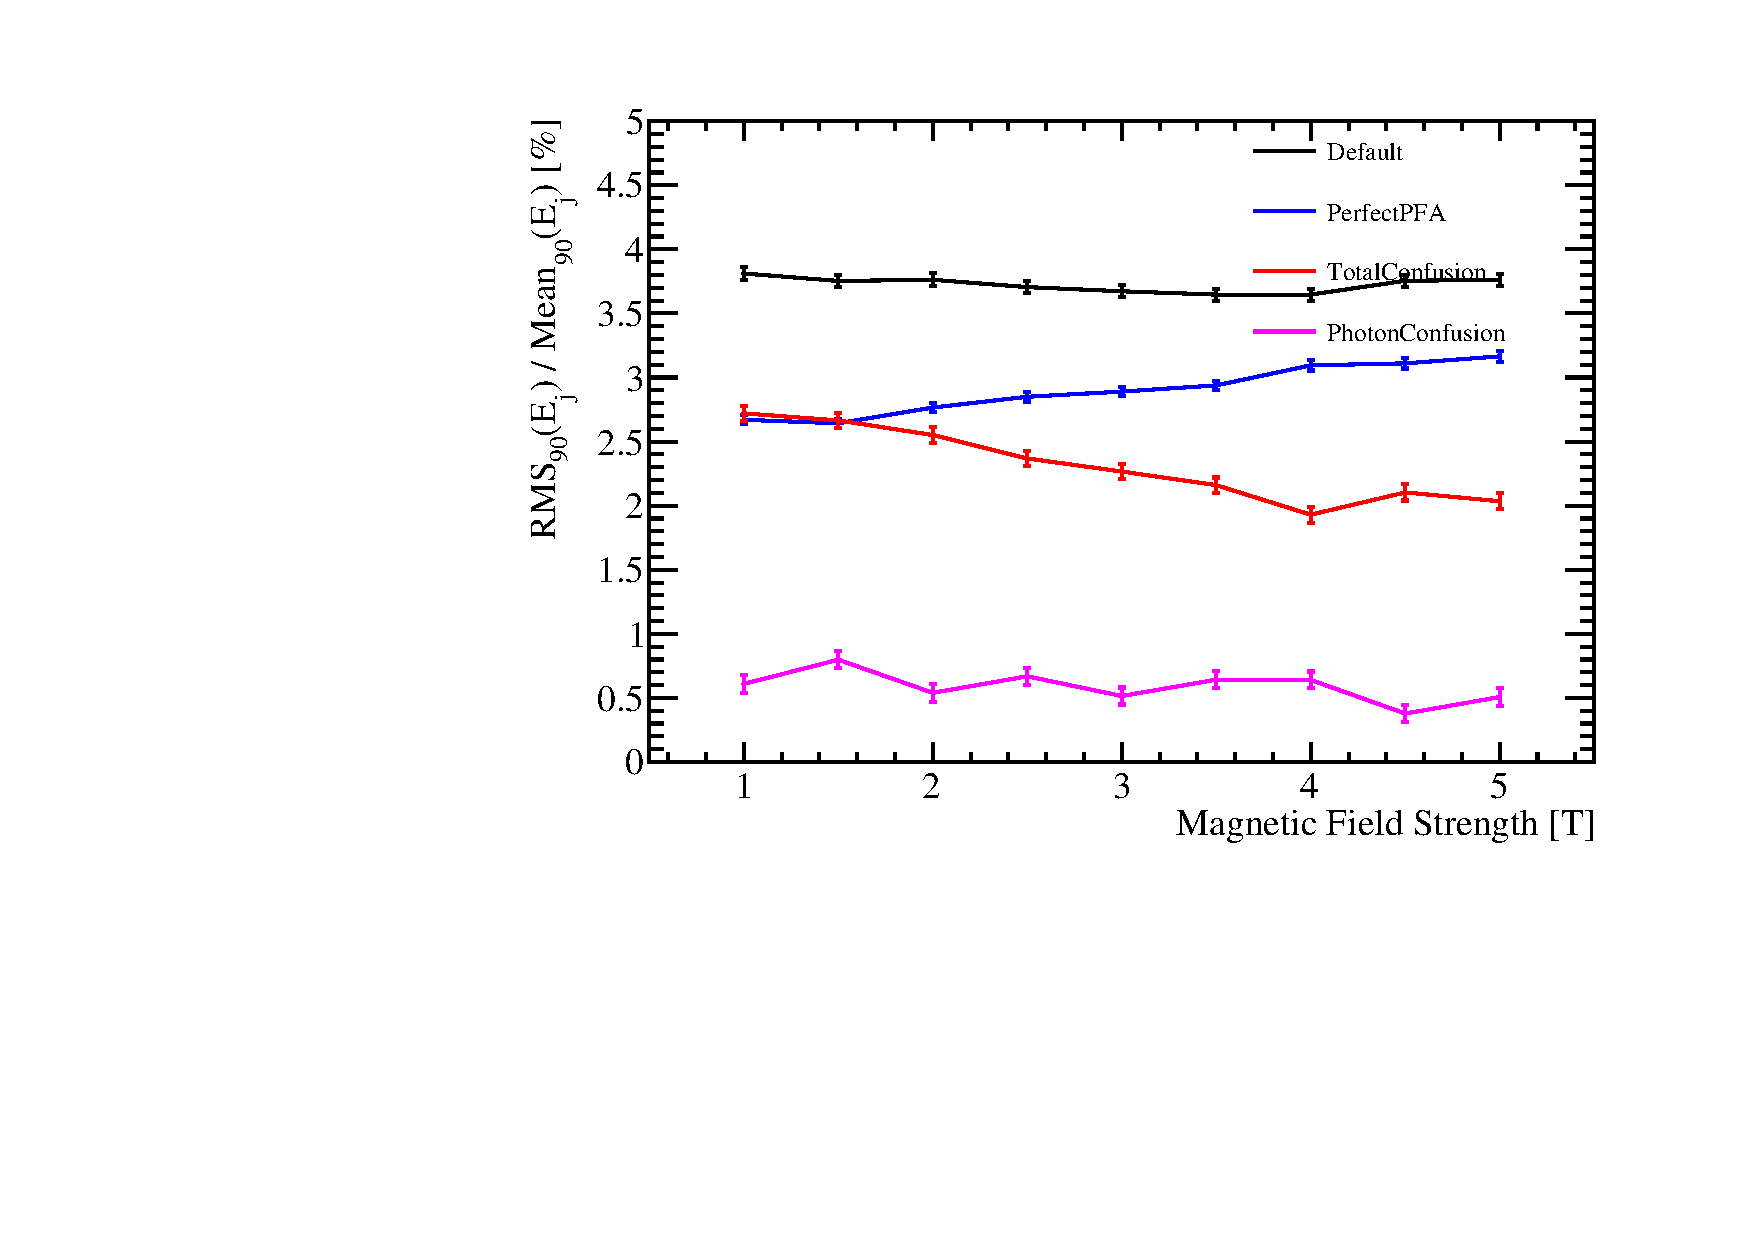
\includegraphics[width=0.5\textwidth]{OptimisationStudies/Plots/JetEnergyResolutions/JER_vs_MagneticFieldStrength_91GeV_DiJet_Breakdown.pdf}}
\subfloat[250 GeV Jets.]{\label{fig:hcalnlayers250break}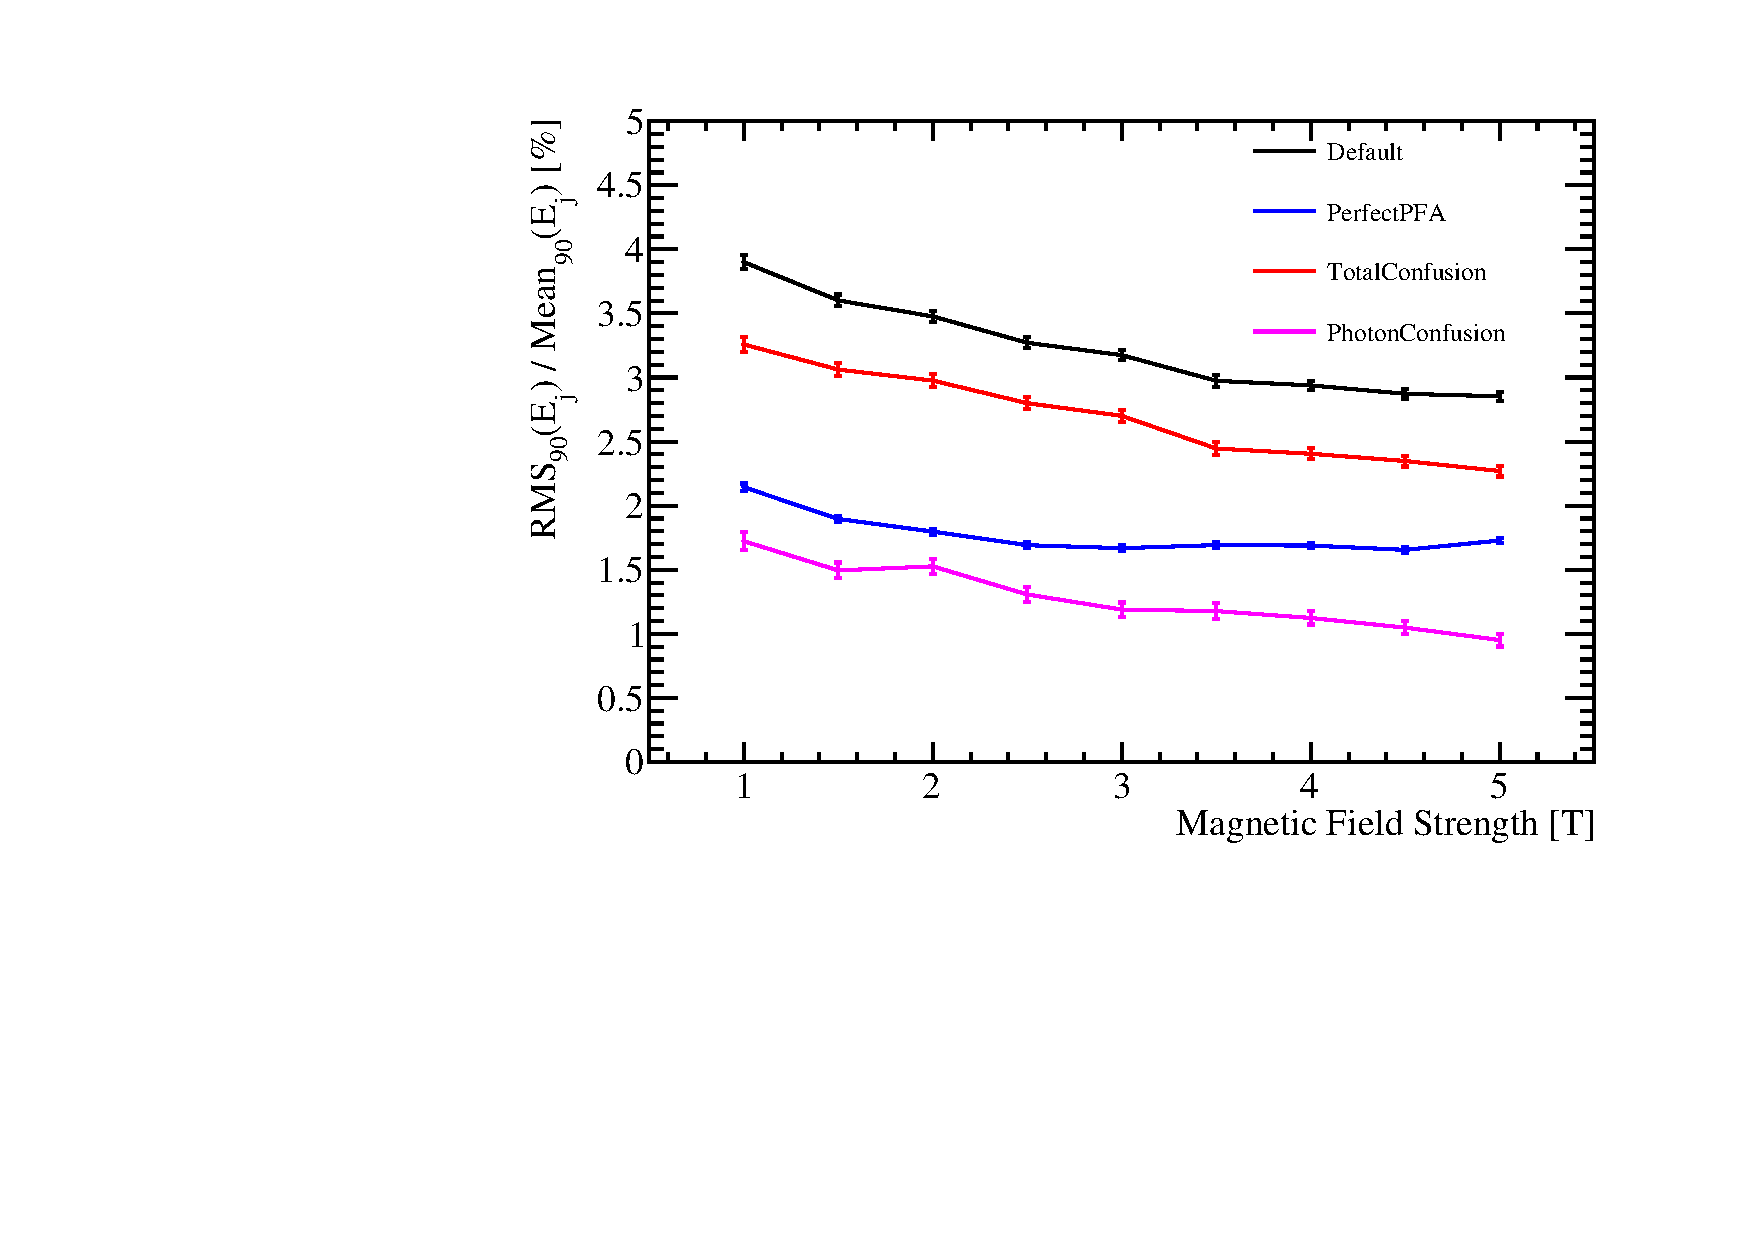
\includegraphics[width=0.5\textwidth]{OptimisationStudies/Plots/JetEnergyResolutions/JER_vs_MagneticFieldStrength_500GeV_DiJet_Breakdown.pdf}}
\caption[Jet energy resolution breakdown as a function of magnetic field strength for 45 and 250 GeV jets.]{Jet energy resolution breakdown as a function of magnetic field strength for 45 and 250 GeV jets.}
\label{fig:bfieldbreak}
\end{figure}

Examination of the decompositions of the jet energy resolution, found in figure \ref{fig:bfieldbreak}, highlights a number of effects.  

The first is a clear reduction in confusion with increasing magnetic field strength.  This is due to a larger separation between charged and neutral hadron energy deposits in the calorimeter as was expected.  

Secondly there is a reduction in intrinsic energy resolution with increasing magnetic field strength for low energy jets, while for high energy jets this trend is reversed.  At low energies the momenta of the charged particles will be low and so the radii of curvature of the helix these particles transverse will be small.  If the radius for a given particle is small enough it will not make it into the calorimeters.  In this case only if the track produced from this particle passes tight selection cuts designed to ensure the track originates from the impact point will the track be used to create a PFO.  Therefor, energy can and will be lost in from events where PFOs are stuck within the tracker.  Given the radii of curvature is inversely proportional to the magnetic field strength, the larger the magnetic field strength the more tracks will be confined to the tracker.  The more tracks that are confined to the tracker, the worse the intrinsic energy resolution becomes as inevitably some tracks fail the quality cuts to form PFOs.  At high jet energies the transverse momentum of the particles will be sufficiently large that the radii of curvatures of the helices formed by charged particles will be enough so that they reach the calorimeters on average.  However, for low magnetic field strengths more particles deposit energy within the same calorimeter cells.  The intrinsic energy resolution plot is determined by associating a single MC particle to each calorimeter cell.  At high jet energies and low magnetic field strengths many of the cells will have energy deposits split between multiple cells and so associating a single MC particle per cell is inaccurate.  This explains why the intrinsic energy resolution degrades slightly in this scenario.  These results are still of interest, however, because the driving term in the jet energy resolution as a function of magnetic field strength is the confusion.

In summary, increasing the magnetic field strength is beneficial to detector performance as it reduces confusion from associating tracks to calorimetric energy deposits from charged particles.  While there is a reduction in the intrinsic energy resolution for low transverse momentum jets with increasing magnetic field strength, this effect is largely offset by the change in confusion.  While the nominal field of 3.5 T gives good performance increasing the field strength is a clear way of making large gains in detector performance.

%========================================================================================

\subsection{Inner ECal Radius}
This section focuses on optimising the inner ECal radius, or the outer tracker radius.  The nominal detector model has an ECal inner radius of 1808 mm and for this optimisation detector models were considered where the ECal inner radii was set to 1208, 1408, 1608 and 2008 mm.  All other detector parameters identical to those of the nominal ILD detector model.

\begin{figure}
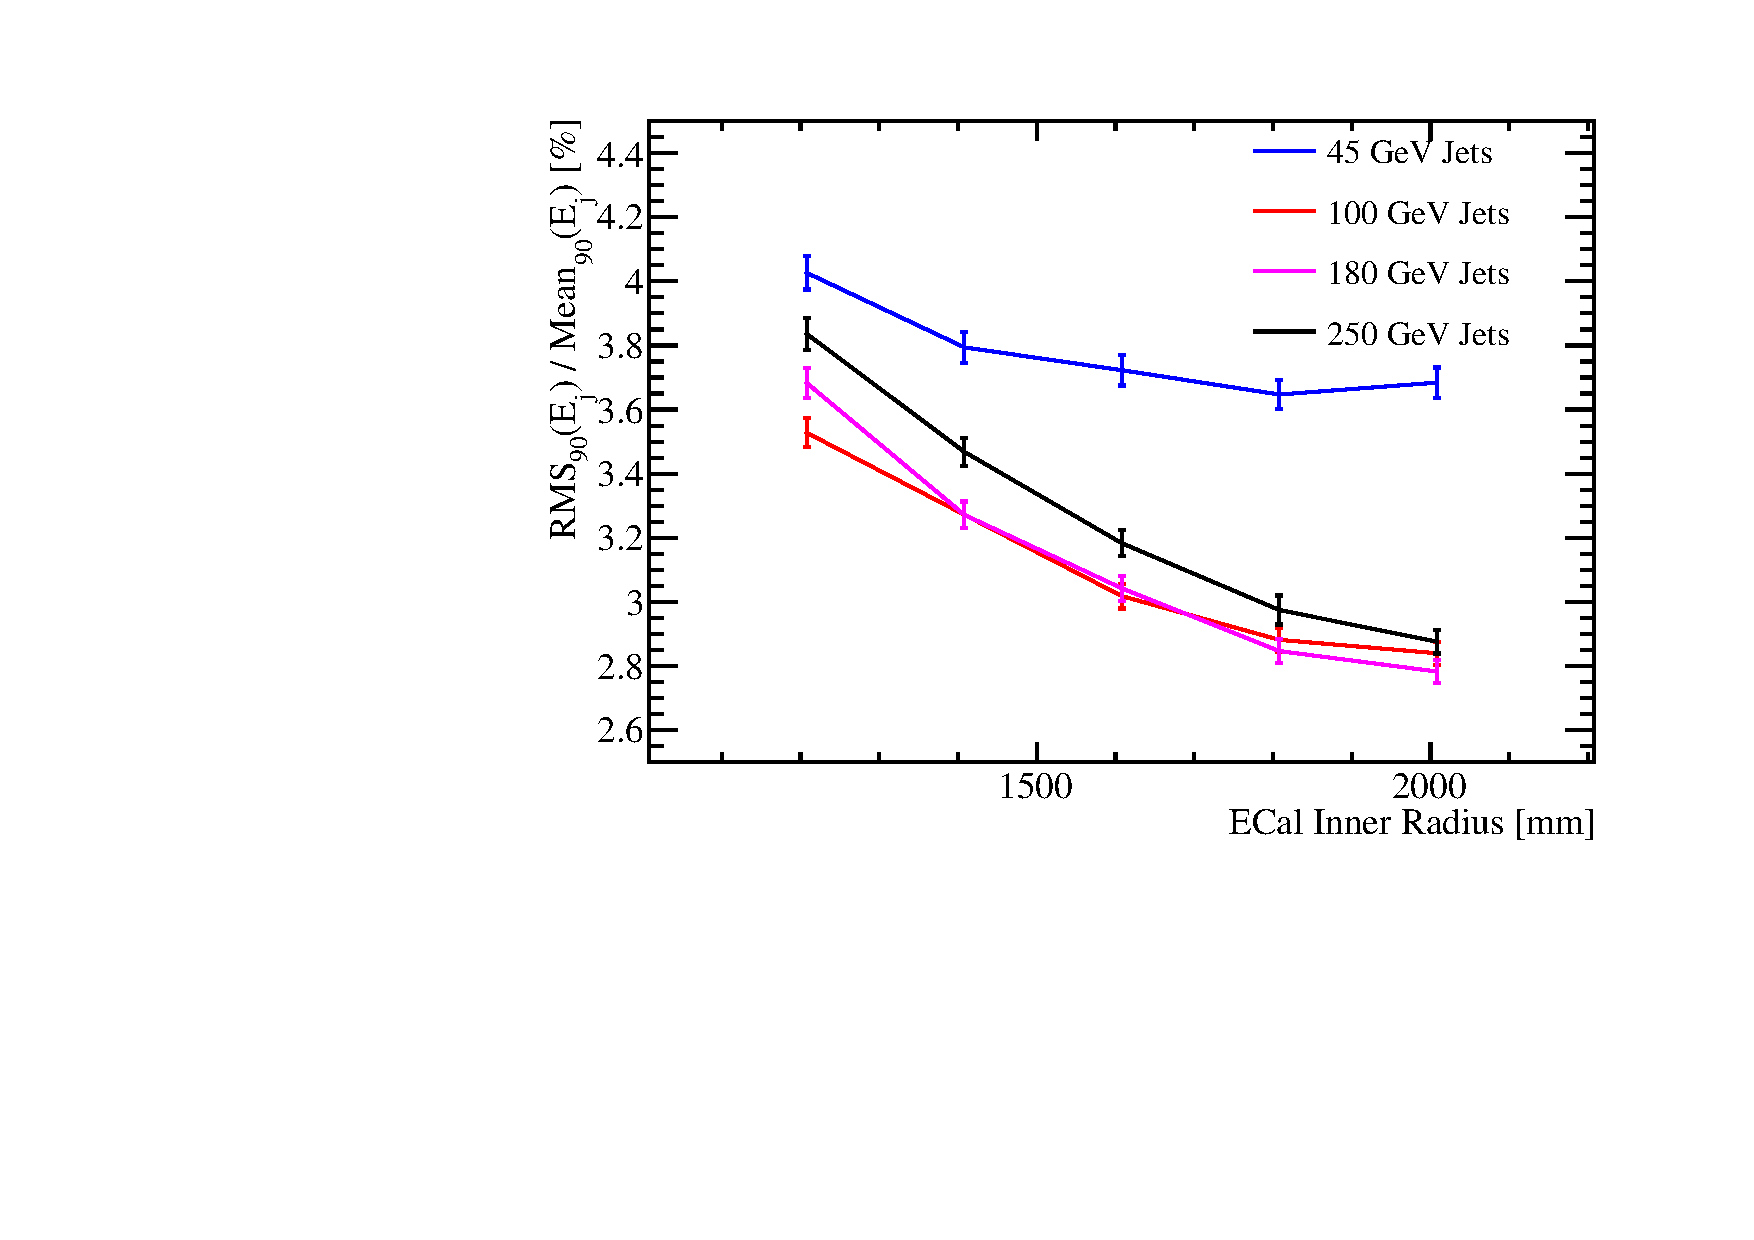
\includegraphics[width=0.5\textwidth]{OptimisationStudies/Plots/JetEnergyResolutions/JER_vs_ECalInnerRadius.pdf}
\caption[Jet energy resolution as a function of ECal inner radius.]{Jet energy resolution is shown for several fixed energy jets as a function of ECal inner radius.}
\label{fig:ecalinnerr}
\end{figure}

The jet energy resolution as a function of ECal inner radius is shown in figure \ref{fig:ecalinnerr} and these results show that a large ECal inner radius was highly beneficial to detector performance.  This is due to the fact that a large tracker gives more time for charged particles to bend due to the magnetic field, which creates a larger separation between calorimetric energy deposits from charged and neutral particles.  This larger separation reduces the confusion when associating calorimetric energy deposits to tracks and so improves the detector performance.  This conclusion is backed up by the decomposition of the jet energy resolution for the low and high energy jets, shown in figure \ref{ig:ecalinnerrbreak}, which explicitly show a reduction in confusion with increasing ECal inner radius.  

The intrinsic energy resolution of the detectors follows the same pattern as was observed in the magnetic field study.  For low energy jets the larger ECal radius means fewer particles make it to the calorimeters and so some PFOs are not reconstructed giving a worse energy resolution.  While at larger jet energies the radii of curvature of the charged particles is sufficiently large as the particles have higher momenta, meaning very few are confined to the tracker and so the intrinsic energy resolution is largely invariant.  There is a small degradation in intrinsic energy resolution at low ECal inner radii due to the association of a single MC particle per calorimeter cell when running the cheated pattern recognition as explained in section \ref{sec:bfield}.  Again, this effect has little bearing on the final conclusions as the change in intrinsic energy resolution across the detector models is a second order effect.  

\begin{figure}
\subfloat[45 GeV Jets.]{\label{fig:hcalnlayers45break}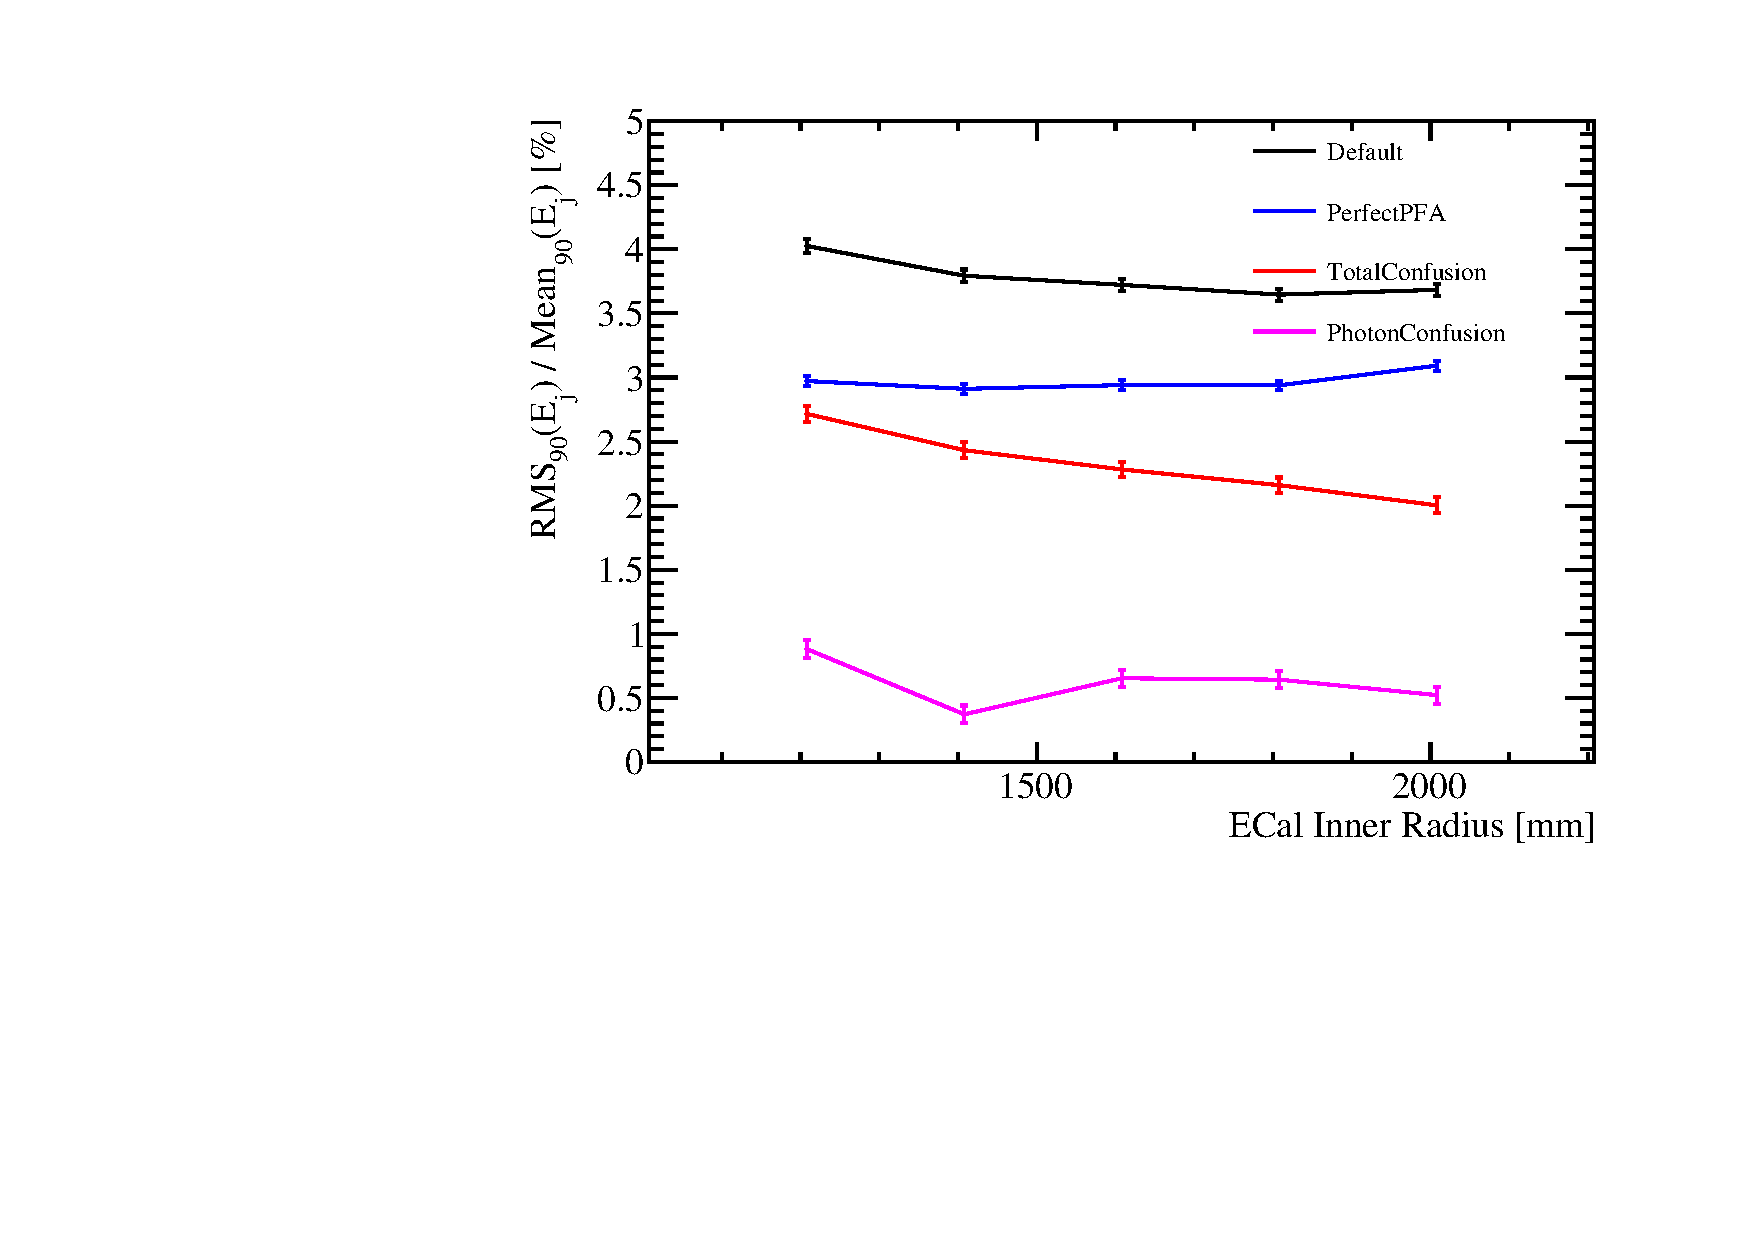
\includegraphics[width=0.5\textwidth]{OptimisationStudies/Plots/JetEnergyResolutions/JER_vs_ECalInnerRadius_91GeV_DiJet_Breakdown.pdf}}
\subfloat[250 GeV Jets.]{\label{fig:hcalnlayers250break}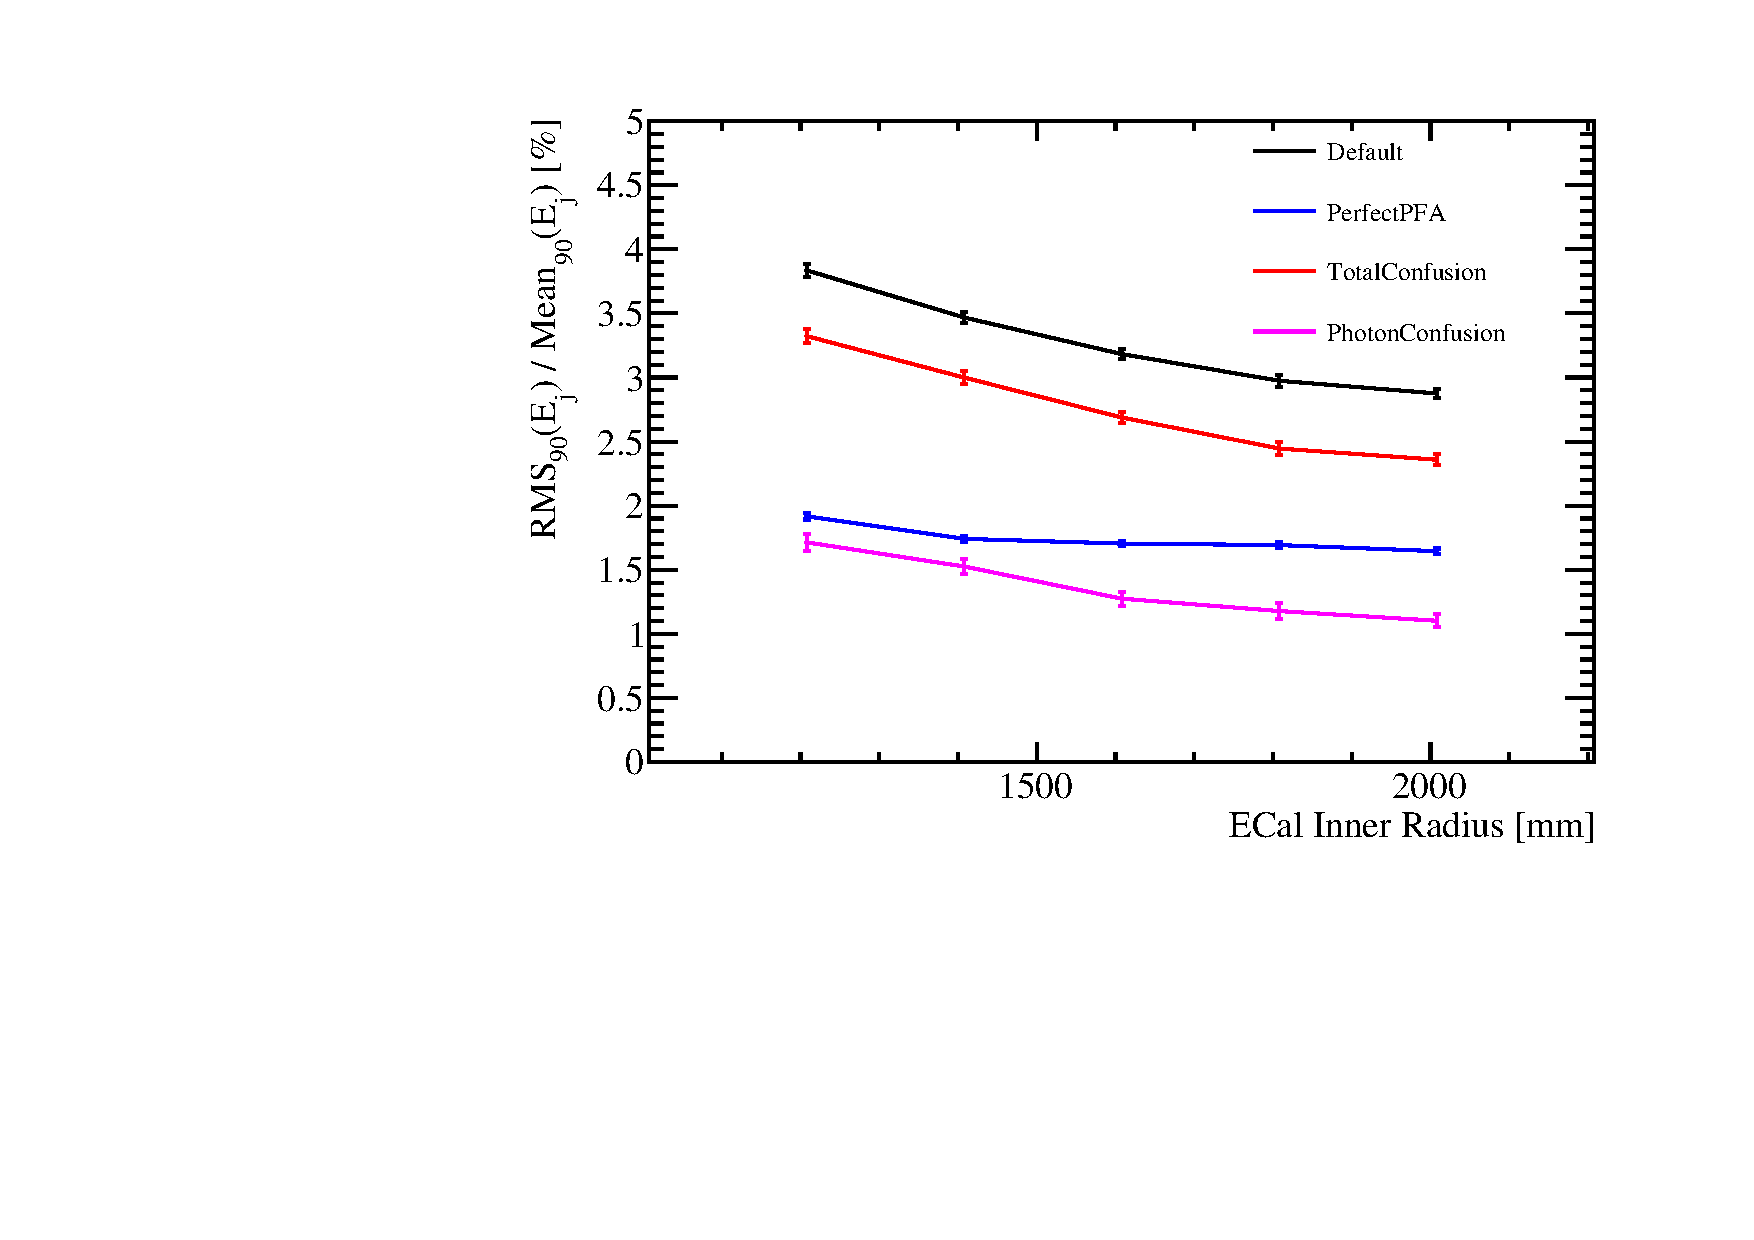
\includegraphics[width=0.5\textwidth]{OptimisationStudies/Plots/JetEnergyResolutions/JER_vs_ECalInnerRadius_500GeV_DiJet_Breakdown.pdf}}
\caption[Jet energy resolution breakdown as a function of ECal inner radius for 45 and 250 GeV jets.]{Jet energy resolution breakdown as a function of ECal inner radius for 45 and 250 GeV jets.}
\label{fig:ecalinnerrbreak}
\end{figure}

In conclusion, increasing the ECal inner radius benefits the jet energy resolution significantly.  This trend is driven by changes to the confusion in associating tracks to calorimetric energy deposits, with a larger ECal inner radius producing a reduction in the confusion as separation of charged and neutral particle energy deposits increases.  

%========================================================================================
%========================================================================================

\section{Conclusions}






